\documentclass{article}
\usepackage[T1]{fontenc}
% \usepackage{utopia}
\usepackage[toc,page]{appendix}
\usepackage{graphicx} % Required for inserting images
\usepackage{amssymb}
\usepackage{amsmath}
\usepackage{amsmath}
\usepackage{makecell}
\usepackage{listings}
\usepackage{xcolor}
\usepackage{subfig}
\usepackage{outlines}
\usepackage{fancyhdr}
\usepackage{titlesec}
\definecolor{refs}{RGB}{31, 82, 204} 
% \definecolor{refs}{RGB}{202, 10, 54} 
\usepackage[colorlinks=true, linkcolor=refs, citecolor=refs, urlcolor=refs]{hyperref}
\usepackage{natbib}
% \bibliographystyle{plainnat} % or any other style

% \usepackage{sourcecodepro}

\lstset{basicstyle=\footnotesize\ttfamily,breaklines=true}
\lstset{framextopmargin=50pt,frame=bottomline}

\definecolor{codegreen}{rgb}{0,0.6,0}
\definecolor{codegray}{rgb}{0.5,0.5,0.5}
\definecolor{codepurple}{rgb}{0.1,0,0.82}
\definecolor{backcolour}{rgb}{0.95,0.95,0.95}

\lstdefinestyle{mystyle}{
    backgroundcolor=\color{backcolour},   
    commentstyle=\color{blue},
    keywordstyle=\color{red},
    numberstyle=\tiny\color{red},
    stringstyle=\color{red},
    basicstyle=\ttfamily\footnotesize,
    breakatwhitespace=false,         
    breaklines=true,                 
    captionpos=b,                    
    keepspaces=true,                 
    numbers=left,                    
    numbersep=5pt,                  
    showspaces=false,                
    showstringspaces=false,
    showtabs=false,                  
    tabsize=1
}

\lstdefinelanguage{Julia}
  {morekeywords={abstract,break,case,catch,const,continue,do,else,elseif,
      end,export,false,for,function,immutable,import,importall,if,in,
      macro,module,otherwise,quote,return,switch,true,try,type,typealias,
      using,while},
   sensitive=true,
   alsoother={},
   morecomment=[l]\#,%
   morecomment=[n]{\#=}{=\#},%
   morestring=[m]{'}{'},%
}[keywords,comments,strings]%


\lstset{
language         = Julia,
  numbers=left,
  stepnumber=1,    
  firstnumber=1,
  numberfirstline=true,
  style=mystyle
}
\renewcommand{\familydefault}{\sfdefault}

% \lstset{%
%     language         = Julia,
%     style=mystyle
% }

% \usepackage{multicol}
\usepackage[a4paper, total={5.7in, 8.6in}]{geometry}

\DeclareMathOperator*{\minimize}{minimize}

% \pagestyle{myheadings}
% \markright{Andrin Rehmann \hfill On page styles\hfill}

\pagestyle{fancy}
\fancyhf{}
\fancyhead[L]{Page \nouppercase{\thepage}} % Bold section name
\fancyhead[R]{\nouppercase{\leftmark}} % Bold page number
\renewcommand{\headrulewidth}{1.3pt}% Default 

% % Define a custom style for section-starting pages
% \fancypagestyle{sectionstyle}{
%     \fancyhf{} % Clear all header and footer fields
%     \fancyhead[L]{\textbf{\leftmark}} % Bold section name
%     \fancyhead[R]{\textbf{\thepage}} % Bold page number
%     \fancyfoot[C]{} % Empty footer
% }

% Customize section titles
\titleformat{\section} % Command to format sections
  {\normalfont\Large\bfseries\color{black}} % Format: font, size, bold, color
  {\thesection} % Label (e.g., "1.2")
  {1em} % Horizontal separation between label and title
  { }% Code preceding the title
  [] % Code following the title (e.g., a horizontal rule)

% Adjust spacing around section titles
\titlespacing*{\section}{0pt}{120pt}{50pt} % Left margin, vertical space before, vertical space after


\begin{document}


\begin{titlepage}
   \begin{center}
      \large
       \textbf{Andrin Rehmann}\\
       \vspace*{0.5cm}
        \Huge
       \textbf{Predicting Dark Matter Initial Conditions}\\
       \large
     \vspace*{0.5cm}
       
        \large
       \vspace{1.5cm}

        Supervisor \\
        Prof. Dr. Robert Feldmann \\

        \vspace{0.5cm}
        Co-supervisor \\
        Dr. Douglas Potter \\
        Dr. Mauro Bernardini 
        
 
       \vfill
            
       Master Thesis for the\\
       \textbf{Specialized Master in Computational Science}
            
       \vspace{0.8cm}
     
       % \includegraphics[width=0.4\textwidth]{university}
            
       Department of Astrophysics\\
       University of Zürich\\
       Switzerland\\
       May 2025
            
   \end{center}
\end{titlepage}

\newpage

\section*{Abstract}

Predicting the initial conditions of dark matter distributions, that evolve into observed cosmic structures when seeded into numerical simulations, remains a critical challenge in cosmology. Traditional methods often rely on an iterative optimization over the numerical solver. Consequently, the computational costs are prohibitive for large-scale simulation. This thesis explores the feasibility of using Fourier Neural Operators (FNOs) — a class of deep learning architectures designed to mimic partial differential equations — to directly predict initial density fields from final-state simulations. We propose an adapted FNO with progressive Fourier mode refinement, paired with a log-growth normalization strategy, to handle the highly heterogeneous density distribution of cosmological dark matter density fields. Trained on N-body simulations generated with PKDGRAV3, the model successfully predicts large-scale structures (low k-modes). However, small-scale nonlinearities (high k-modes) remain challenging due to information loss in grid-based discretization and chaotic gravitational interactions. We demonstrate that autoregressive training with skip connections improves predictions but is limited by memory constraints. While the method falls short of replacing traditional optimization-based approaches, it offers a solid foundation for future work. 

\newpage 

\tableofcontents

\newpage


\section{Introduction}


When observing structures in the universe, we see a static structure of matter. While the nature of the speed of light allows us to peer into the past state of the universe, for each region of space, we can only observe a single state. Unlike many process on earth, we cannot hardly observe changes in the cosmos, as the timescales of such processes are far bigger than human lifespans. Nevertheless, understanding their evolution in time is absolutely crucial to understand the fundamental physics of the cosmos For example, to find answers to the mystery of dark energy. One available option are numerical simulations of matter, that are based on the known fundamental physics. To this end, we generate random matter density distributions that mimic the distributions of the very early stages of our universe, which are then evolved in time by computing and applying the effects of gravity. Ideally, instead of starting with random initial states that are only correct in terms of the underlying distribution, it would be far more helpful to begin with initial states that evolve into structures that are observed today over the course of numerical simulation. 

Simulating in the forward-time direction is, at least from a mathematical perspective, a solved problem. Naturally, some dynamics in the universe are not thoroughly understood, while others are simplified to accommodate limited computational resources. But we can solve N-Body systems with high accuracy and generate simulated universes that fundamentally resemble our observations. From a computational perspective, the problem is challenging, especially when a high resolution of the simulated universe is desired. Because if we choose to compute all interacting forces individually, we end up with a runtime that scales quadratically with the number of particles that are used to discretize the density field. Nowadays, there exists a range of efficient solvers for large-scale N-Body simulations \citep{potter2017pkdgrav3, springel2021simulating, garrison2021abacus}, which leverage methods such as the multipole expansion to reduce the computational complexity to scale linearly with the number of particles. 

Going back in time and trying to obtain matching initial conditions for a given final state is complicated. In theory, the numerical solvers could be reversed; however, due to the highly nonlinear effects and observational noise, this approach is not applicable \citep{jasche2013bayesian}. Previously proposed methods often rely on Bayesian optimization, where at first a random guess for the initial conditions is fed into the forward simulation. By comparing the resulting distribution against the desired distribution, we can evaluate the correctness of this initial state, which provides a first estimate of the multidimensional surface of the objective to be optimized. If we define our objective as a loss, we then need to gather more information to find a minimum of this surface. By repeating the experiment with various initial conditions, exploring the surface to gather information and exploiting available information to move closer to minima, we can find suitable solutions. Approximating the loss surface for high-dimensional problems, which in our this case translates to higher resolutions of density distributions, can become computationally infeasible \citep{djolonga2013high}. By implementing the forward solver in a differentiable manner, we can replace the Bayesian optimization with a gradient-based optimization. Since those gradients provide us information about the slope of the loss surface, we can immediately start moving in a direction of lower loss. Such an approach is often preferred in high dimensional optimization problems. We can also enrich the approximations of the loss surface of Bayesian approaches with the gradient information. Such hybrid approaches have been popular and can reconstruct the initial density field down to small scales \citep{wang2014elucid}.

In this master’s thesis, we examine the application of deep learning methods to predict the initial conditions. More precisely, we propose a surrogate model which learns to integrate back in time using a purely data-driven training method. The big advantage of such a surrogate, is once training is complete, inference does not rely on an optimization process. All the methods we have described before, rely on a complete forward solve of the n-body problem in each optimization iteration, resulting in a computationally demanding optimization process which has to be repeated for each given data sample.

We propose to learn a function capable of mapping between two dark matter density fields. The input of this function is the density field of the final state of the simulation, and the output is the initial condition. Deep learning methods have been applied successfully in many domains, ranging from medicine \citep{wang2019deep} to physics \citep{thuerey2021physics} and social sciences \citep{orabi2018deep}. More recently, they have also become more popular in cosmology \citep{escamilla2020deep, mathuriya2018cosmoflow, bernardini2022ember}. However, at the time of writing this thesis, leveraging deep learning for predictions across time steps in N-Body simulations is a completely novel field and presents exciting new challenges and opportunities.

To limit the computational demands and time efforts of this thesis, we have restricted the deep learning model to a density field that is discretized on an equidistant grid. This enables us to apply well-studied convolutional-based neural network architectures. We propose a purely data driven approach, where the ground truth is based on several evaluations of an N-Body simulation using the PKDGRAV3 code \citep{potter2017pkdgrav3}. Converting the particles into a grid-based density field, inevitably degrades the quality of the data, as potentially multiple particles are cramped into a single grid cell. Hence, if we consider information preservation, ideally we would feed the entire array of particles and their masses into the neural network. However, graph-based approaches are a more novel field and arguably more complex to apply. Furthermore, most GNN techniques depend on up-sampling the input into high dimensional latent spaces \citep{wu2020comprehensive}, making it difficult to fit models into the available GPU memory. Contrary, grid-based methods are well researched and perform well with lower order latent space representations.

In this thesis, we provide a brief explanation of important cosmological theories and an introduction to the computational methods used to solve the N-Body problem. We then introduce the concept of gradient-based optimization, automatic differentiation and convolutional based networks architectures. Following this, we provide a more precise problem definition and an overview of comparable methods. We then explain the applied method in detail, present results and provide solutions to problems. Finally, we provide some implementation details and draw a conclusion.

\newpage


\section{Dark Matter N-Body Simulations}
Dark matter constitutes 85\% of the total mass in the universe \citep{carroll2007dark}. Consequently, dark matter simulations are crucial to explaining galaxy formation in the universe. Since dark matter is not affected by electromagnetic fields or atomic forces, simulations are relatively simple, as the only interactions to consider are due to gravitational forces. Usually, dark matter N-Body simulations rely on initial conditions that constitute a Gaussian random field perturbed to align with known metrics during the early stages of the universe. These initial conditions are then evolved under the influence of the governing equations, which, in the case of dark matter, describe the influence of gravity using a numerical solver. Finally, when the simulation has reached the end state, usually representing the current time of the universe, we can compare observations with the simulation, with the advantage of being able to trace objects back in time.

The simulated universe is contained in a box of fixed size with periodic boundary conditions. Essentially, we are looking at a density field \(\rho(\mathbf{x}, t) \colon \mathbb{R}^3 \times \mathbb{R} \rightarrow \mathbb{R}\). This is often represented as \(\delta(\mathbf{x}, t) \colon \mathbb{R}^3 \rightarrow \mathbb{R}\), the density contrast field is

\begin{equation}
    \delta(\mathbf{x}) = \frac{\rho(\mathbf{x}) - \overline{\rho}}{\overline{\rho}}.
\end{equation}

And conversely

\begin{equation}
    \rho(\mathbf{x}) = \overline{\rho} \cdot \delta(\mathbf{x}) + \overline{\rho}.
\end{equation}

We can also represent the density field using a set of unstructured particles, where each particle has a position \(\mathbf{x}(t) \in \mathbb{R}^3\) and a mass \(m(t) \in \mathbb{R}\). Such a particle is not equivalent to a physical object such as a planet, star, or galaxy. The particle represents a more abstract notion of mass, where the number of particles and their corresponding masses depend on the resolution and scale of the simulation.

\subsection{Comoving Coordinates}
Since the universe is expanding over time, performing computations using real physical distances can be tricky, as the simulation box size needs to increase over the course of the simulation. Most notably, when using floating-point operations, the precision of computations varies depending on the magnitude of the numbers involved. By using a comoving coordinate frame, the mock universe remains constant, allowing us to fit the entire simulation in a static box with fixed boundaries and simultaneously accounting for the expansion of the universe. Overall, this approach significantly simplifies the overall method. We denote a coordinate in the comoving coordinate space as \(\mathbf{x}\) and in the proper or physical distance as \(\mathbf{x}_p\). The two are related by the expansion factor \(a(t)\) \citep{schutz2003gravity}:

\begin{equation}
    \mathbf{x}_p = \mathbf{x} \cdot a(t).
\end{equation}

The expansion factor is governed by the Friedmann equations, which can be solved for any point in time. The expansion factor correlates positively with the age of the universe, as the universe is expanding. However, the rate of expansion is not constant over time; it has changed throughout the history of the universe, particularly influenced by dark energy and matter content. Still, the expansion factor itself is monotonically increasing over time. In other words its slope is always larger or equal to zero.

\subsection{Time}

Due to the correlation between time and the expansion factor \(a(t)\), it is often used to describe the state of a simulation along with the three-dimensional spatial coordinates. Alternatively, the redshift \(z\), which is closely related to the expansion factor, can also be used to describe the state. The physical phenomena of Redshift occurs when the emitting source is moving away from the observer, while the opposite is termed blue shift. The correlation between redshift and time is related to the expansion of the universe. Due to the expansion of the universe, objects that are further away from the Earth are moving away faster; hence their redshift is more pronounced. Furthermore, light sourced from objects that are far away was emitted a long time ago, hence an increased redshift correlates with observation further back in time of the history of the universe. We can relate the expansion factor \(a\) and the redshift \(z\) to each other with the equation

\begin{equation}
    \label{eq:redshift}
    1 + z = \frac{a_{\text{now}}}{a_{\text{then}}}.
\end{equation}

\subsection{Units and Scale}

A parsec (pc) is a unit of distance used in astronomy, approximately equivalent to 3.26 light-years. The term is derived from the method of parallax, which measures the apparent shift in position of a nearby star against the distant background when observed from two different points in Earth's orbit around the Sun. A megaparsec (Mpc) corresponds to one million parsecs, a scale more convenient for expressing intergalactic distances. For context, the size of the observable universe is estimated to be around 28.5 gigaparsecs (Gpc) \citep{bars2010extra}.

The Hubble constant \(H_0\) is a measure of the rate of expansion of the universe. It is traditionally expressed in units of kilometers per second per megaparsec (km/s/Mpc). However, the precise value of the Hubble constant is subject to some uncertainty due to differing measurements and methodologies, such as those derived from the Cosmic Microwave Background and those based on local observations. As a result, a dimensionless parameter, the Hubble constant \(h\), is often used in equations to express values normalized by a typical value of 100 km/s/Mpc. This allows us to account for uncertainties and make comparisons across different cosmological models and data sets more conveniently. By employing \(h\), we can incorporate new measurements of \(H_0\) without needing to completely overhaul current cosmological calculations, thus enabling ongoing refinements to our understanding of the universe's expansion dynamics.

\subsection{Power Spectrum}
\label{power-spectrum}
An important measure in cosmology is the matter power spectrum, which provides insights into the distribution of matter in the universe across different scales. It is defined as the Fourier transform of the autocorrelation function

\begin{equation}
\xi(r) = \frac{1}{L^3} \sum_{\mathbf{x}} \delta(\mathbf{x}) \delta(\mathbf{x} + \mathbf{r}).
\end{equation}

The autocorrelation function, \(\xi(r)\), captures the amount of matter located at a given distance \(r\), offering a way to quantify the degree to which mass in the universe is clumped together. Essentially, it describes the likelihood of a point of matter at one location being encountered at a distance \(r\) compared to a random distribution. The power spectrum, which is more directly used in cosmological studies, is then defined as \citep{cui2008ideal}

\begin{equation}
    P(\mathbf{k}) = \langle |\delta(\mathbf{k})|^2 \rangle,
\end{equation}

where the angle brackets denote the ensemble average. The power spectrum is dependent on the redshift, representing how structures in the universe evolve over time. Using various techniques, we can approximate the power spectrum of the universe at different redshifts \(z\). 

\begin{itemize}
    \item Linear Power Spectrum: This is the simplest approximation and is valid at large scales where gravitational interactions have not yet led to complex structures. The linear power spectrum helps model the initial conditions of the universe in the early universe.
    \item Nonlinear Power Spectrum: As the universe evolves, gravitational collapse leads to the formation of larger structures like galaxies and galaxy clusters. These nonlinear effects become significant on smaller scales, where the assumptions of the linear approximation break down. The nonlinear power spectrum attempts to capture these complex interactions and provides a more accurate representation of the matter distribution in the universe at present times and on smaller scales.
    \item Zel'dovich Approximation: This approach is an intermediate approximation that adds some sophistication to the linear model by accounting for the initial displacement and momentum of particles. It predicts the formation of cosmic structures like sheets and filaments, often referred to as the \textit{cosmic web} by considering the initial velocity fields of matter. The Zel'dovich approximation is particularly useful in describing the early stages of gravitational collapse and provides insights into the large-scale structure dynamics beyond what the linear theory offers \citep{schneider1995power}.
\end{itemize}


These aforementioned approximations of the power spectrum are illustrated in Figure \ref{fig:power-z}. Here we plot the different power spectrum approximations for redshifts of 49, 10, 3, and 0 (present day).

\begin{figure}[h]
    \centering
    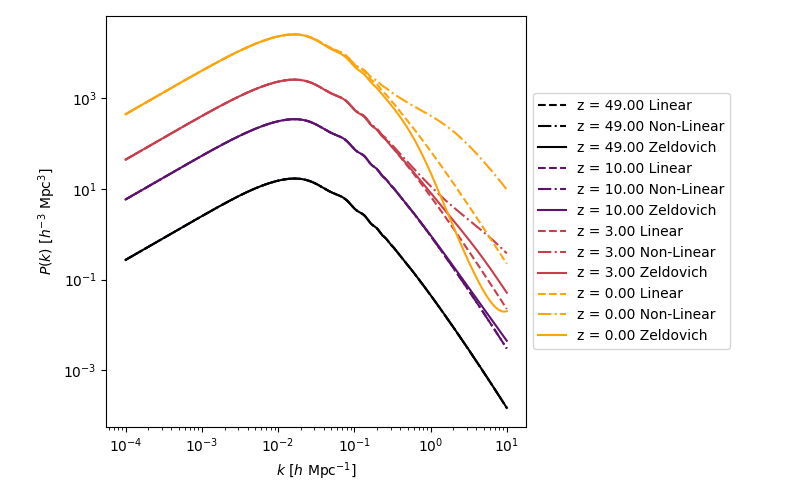
\includegraphics[width=0.75\linewidth]{img/power_spectrum.png}
    \caption{Different power spectrum approximations for redshifts 49, 10, 3, and 0 (present day): linear, nonlinear, and Zel'dovich approximations.}
    \label{fig:power-z}
\end{figure}

\subsection{Mass Assignment}
\label{mass-assignment}

\begin{figure}[h]
    \centering
    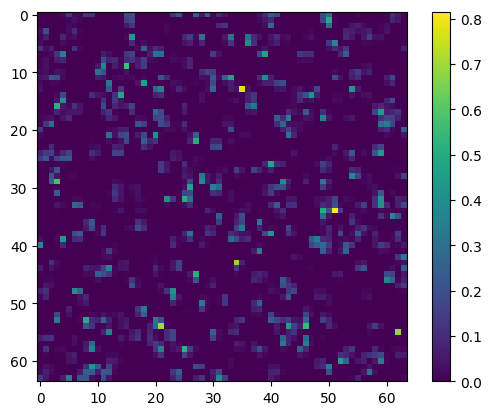
\includegraphics[width=0.5\linewidth]{img/cic.png}
    \caption{CIC mass assignment from cosmax.}
    \label{fig:cosmax-cic}
\end{figure}


In particle mesh method based N-Body simulations, the density field is primarily stored as an unstructured particle array, where each particle is associated with a mass. However, the particles need to be converted from the unstructured representation to a discretized grid to compute the gravitational potential field using a fast spectral method. This conversion is also useful for analysis, for example to compute the power spectrum of a set of unstructured particle positions and masses. In our case, we leverage the conversion to be able to work with the density field as a regular grid for a direct application of grid based neural network. The mapping, also commonly referred to as mass assignment, works by splatting the particles masses at their current positions onto a discrete grid. A widely used algorithm for the mass assignment problem is the cloud in a cell (CIC) mass assignment method. Here, the mass of each particle is distributed to its nearest grid points based on a linear interpolation. This method is an improvement over the nearest-grid-point (NGP) assignment, which can introduce higher artificial discreteness in the density field. 

\subsection{Governing Equations}

In the N-body approach, we describe the particle acceleration as

\begin{equation}
    \mathbf{a}(\mathbf{x}_i, m_i) = -\nabla \Phi(\mathbf{x}_i),
\end{equation}

and the velocity as

\begin{equation}
    \label{eq:velocity}
    \mathbf{v}(\mathbf{x}_i, m_i, t) = \int_0^{t} -\nabla \phi(\mathbf{x}_i) dt.
\end{equation}

Here $\Phi$ is the gravitational potential, which does depend solely on the position and the time. Hence, it can be written expressed as a scalar potential field $\phi(\mathbf{x}) \colon \mathbb{R}^d \rightarrow \mathbb{R}$. The above gives use six ODE equations, for each quantity, position and velocity, there is an equation for each of the 3 dimensions. The gravitational potential $\phi$ can be computed by solving the Poisson equation

\begin{equation}    
    \label{eq:potential-poisson}
    \nabla^2 \phi(\mathbf{x}) = 4 \pi G \rho(\mathbf{x}).
\end{equation}


Alternatively, the forces can be computed directly, meaning all \(N\) to \(N\) interactions are considered without the need to first compute the gravitational potential. This approach involves calculating the pairwise gravitational forces between all particles. The force \(\mathbf{F}_i\) on a particle \(i\) can be calculated by summing the contributions from all other particles \(j\), expressed as

\begin{equation}
    \mathbf{F}_i = -G m_i \sum_{j \neq i} m_j \frac{\mathbf{x}_i - \mathbf{x}_j}{|\mathbf{x}_i - \mathbf{x}_j|^3}.
\end{equation}

Applying this approach to \(N\) particles, results in a computational complexity of \(O(N^2)\) using with naive implementation. We will explain strategies to reduce the computational complexity in section \ref{nbody}. But first, let us discuss how to set up the initial conditions for the N-Body problem.

\subsection{Initial Conditions}

Since predicting the initial conditions is the main target of our thesis, we examine the classical method to generate such initial conditions with a specific example. The method can be broken down into two steps. First, we initialize the Lagrangian particle position $\mathbf{q} \in \mathbb{R}$ on a Cartesian equidistant regular grid. We then perturb the particle positions, by applying a displacement field $\mathbf{s}$ with specific characteristics to obtain the Eulerian particle positions $\mathbf{x}$ using \citep{bertschinger1995cosmics}

\begin{equation}
    \mathbf{x} = \mathbf{q} - D_{+}(a)\mathbf{s}(\mathbf{q}).
\end{equation}

Here $D_+$ is the linear growth function and $\mathbf{s}$ the displacement field. The linear growth factor $D_+$can be approximated by  \citep{carroll2001cosmological}

\begin{equation}
    D_+(a) = \frac{\frac{5}{2} a \Omega_M}{
    \Omega_m^{\frac{4}{7}} - \Omega_{\Lambda} + ( 1 + \frac{\Omega_M}{2})(1 + \frac{\Omega_{\Lambda}}{70})
    }.
    \label{eq:growth}
\end{equation}

$\Omega_M$ is the mass density constant of the universe, $\Omega_{\Lambda}$ is the fraction of mass attributed to dark energy and $\Omega_{rel}$ describes the mass attributed to electromagnetic energy and neutrinos. Together, the constants sum up to the total density parameter $\Omega$ \citep{carroll2017introduction}. With cold dark matter simulations, the initial particle velocities depend solely on the particle positions. Subsequently, the velocity can be computed with

\begin{equation}
    \mathbf{v} = \frac{d D_+(a)}{d t} \cdot \mathbf{s}(\mathbf{q}).
\end{equation}



% When the position is known, the potential is then given by

% \begin{equation}
%     \mathbf{p} = -(a - \Delta \frac{a}{2})^2 \dot{D}_+ (a - \Delta \frac{a}{2}) \mathbf{s}(\mathbf{q}),
% \end{equation}

% where $a$ is the initial expansion factor and $\Delta a$ is its step.

The displacement map $\mathbf{s}$, changes the Lagrangian particle positions just enough, such that the resulting distribution follows the desired matter Power Spectrum distribution. Hence, the displacement map is dependent on the matter power spectrum and can be computed using

\begin{equation}
    \mathbf{s}(\mathbf{q}) = \alpha \sum i \mathbf{k} c_k e^{i \mathbf{k} \cdot \mathbf{q}}
\end{equation}

whereas $\mathbf{k}$ and $c_k$ are discrete realizations of a cosmological power spectrum on a grid in Fourier space.

\subsubsection{IC Generation}


\begin{figure}[h]
    \centering
    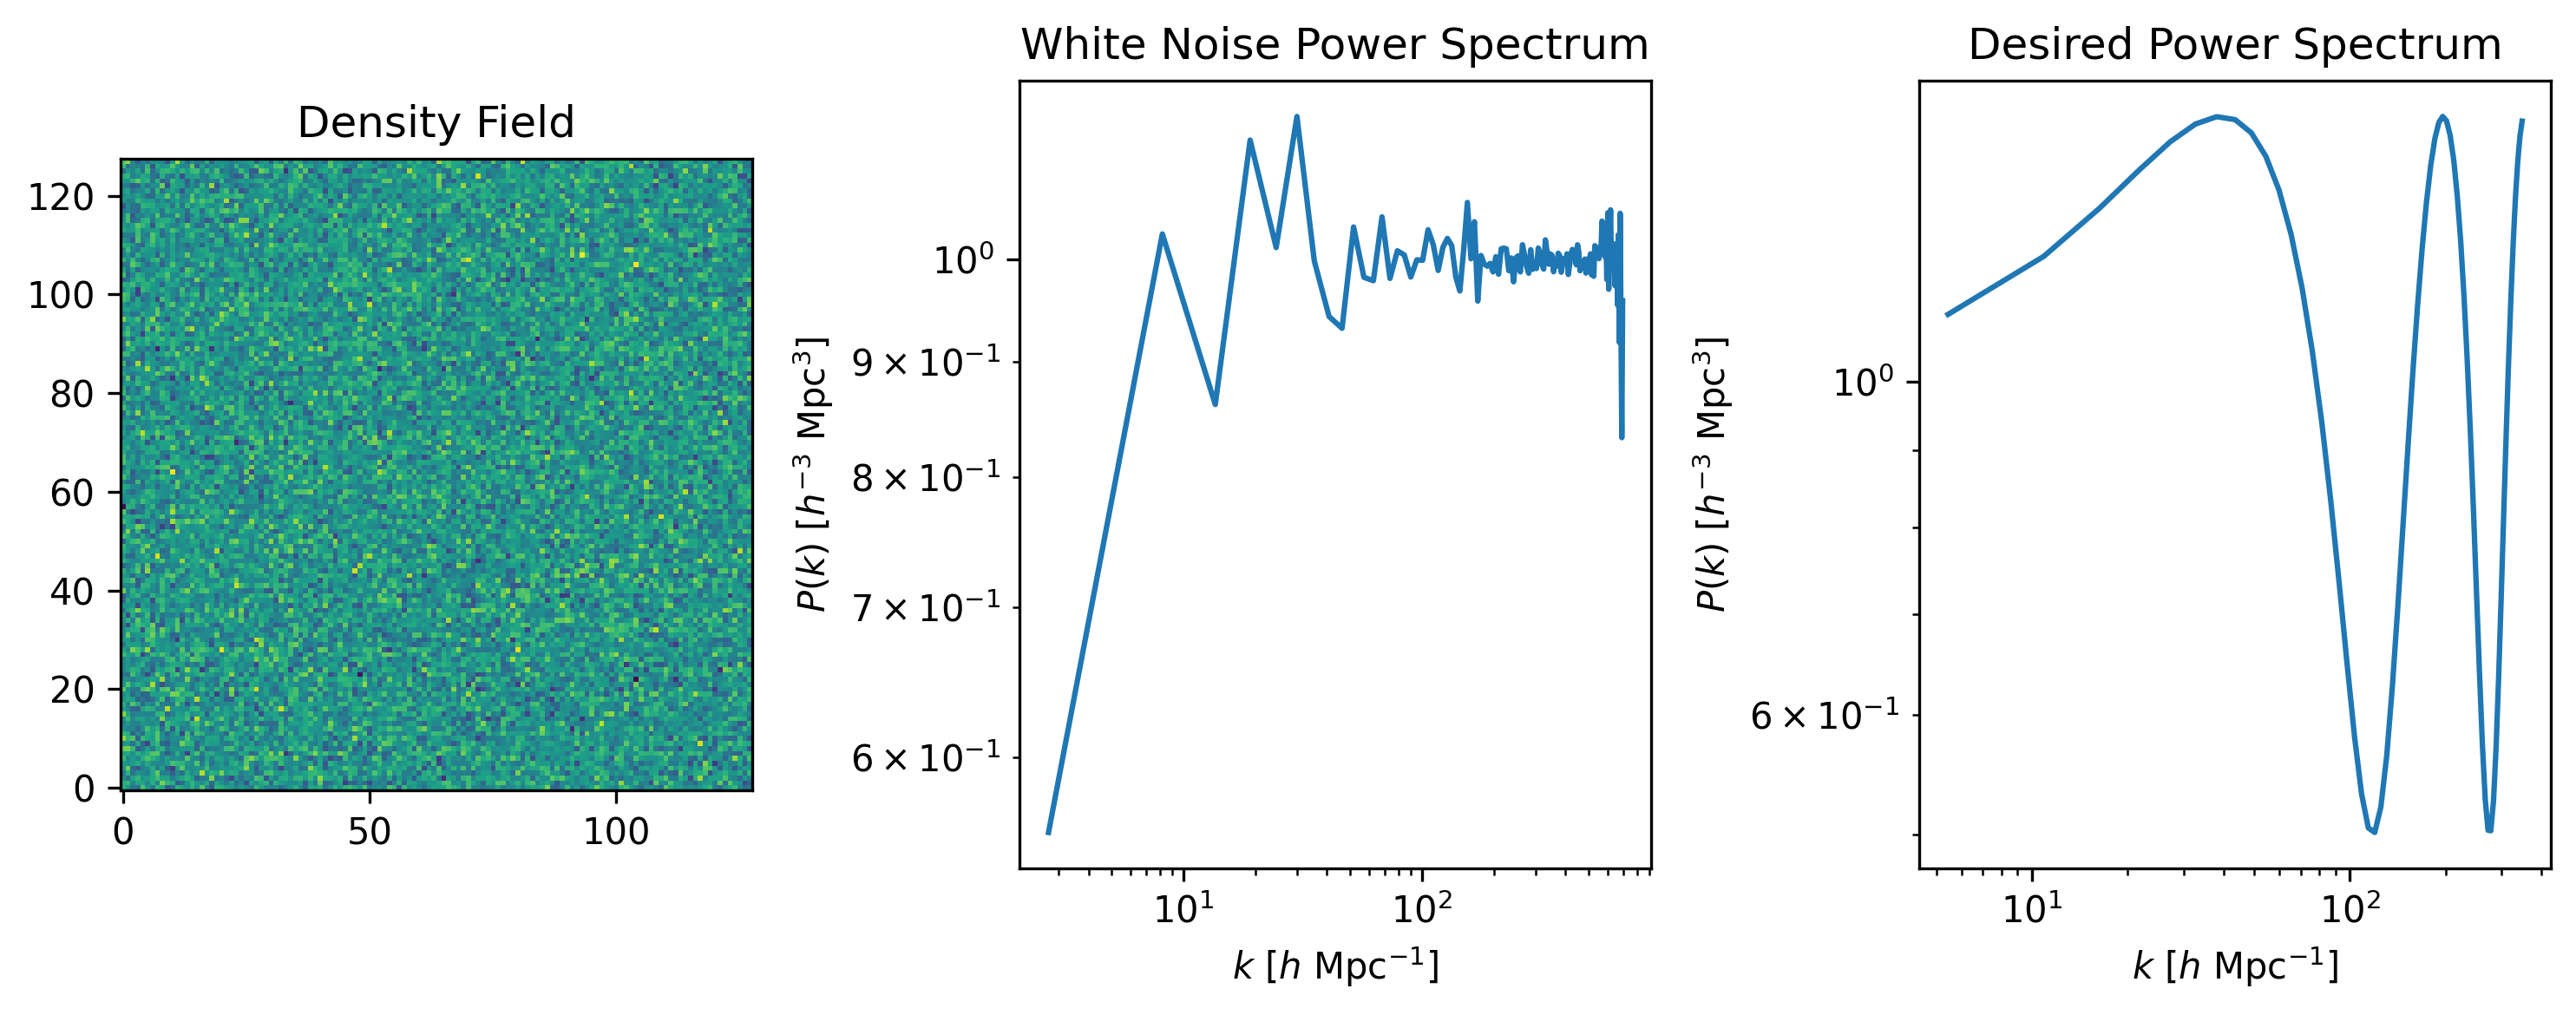
\includegraphics[width=0.7\linewidth]{img/IC_sine_setup.png}
   \caption{Random distribution, its power spectrum, and the desired power spectrum.}
\label{fig:random}
\end{figure}

To compute the initial conditions, a power spectrum approximation as seen in section \ref{power-spectrum} can be used. For demonstration we imprint a power spectrum that is defined by

\begin{equation}
    P(k) = \frac{\sin(k \cdot 0.04)}{2} + 1
\end{equation}
into the white noise density field with a constant power spectrum of one. The setup can be seen in figure \ref{fig:random}, where we see the white noise, its power spectrum and the desired power spectrum. We then compute the correlation kernel by taking the square root \citep{prunet2008initial}

\begin{equation}
    A(\mathbf{k}) = \sqrt{P(\langle \mathbf{k} \rangle)}.
\end{equation}

Note $\mathbb{k}$ is the wave vector and $k$ is the wave magnitude. Hence we denote

\begin{equation}
    \langle k \rangle = \sqrt{\mathbf{k}_x^2 + \mathbf{k}_y^2 + \mathbf{k}_z^2}
\end{equation}

where the subscripts $x$, $y$ and $z$ denote the components of the vector $\mathbf{k}$. The correlation kernel can be seen in the center plot of figure \ref{fig:cocrr}. We can observe the original function as it is transformed into a 3D kernel by looking up its value at the corresponding lengths of the wave vector $\mathbf{k}$.


\begin{figure}[h]
    \centering
    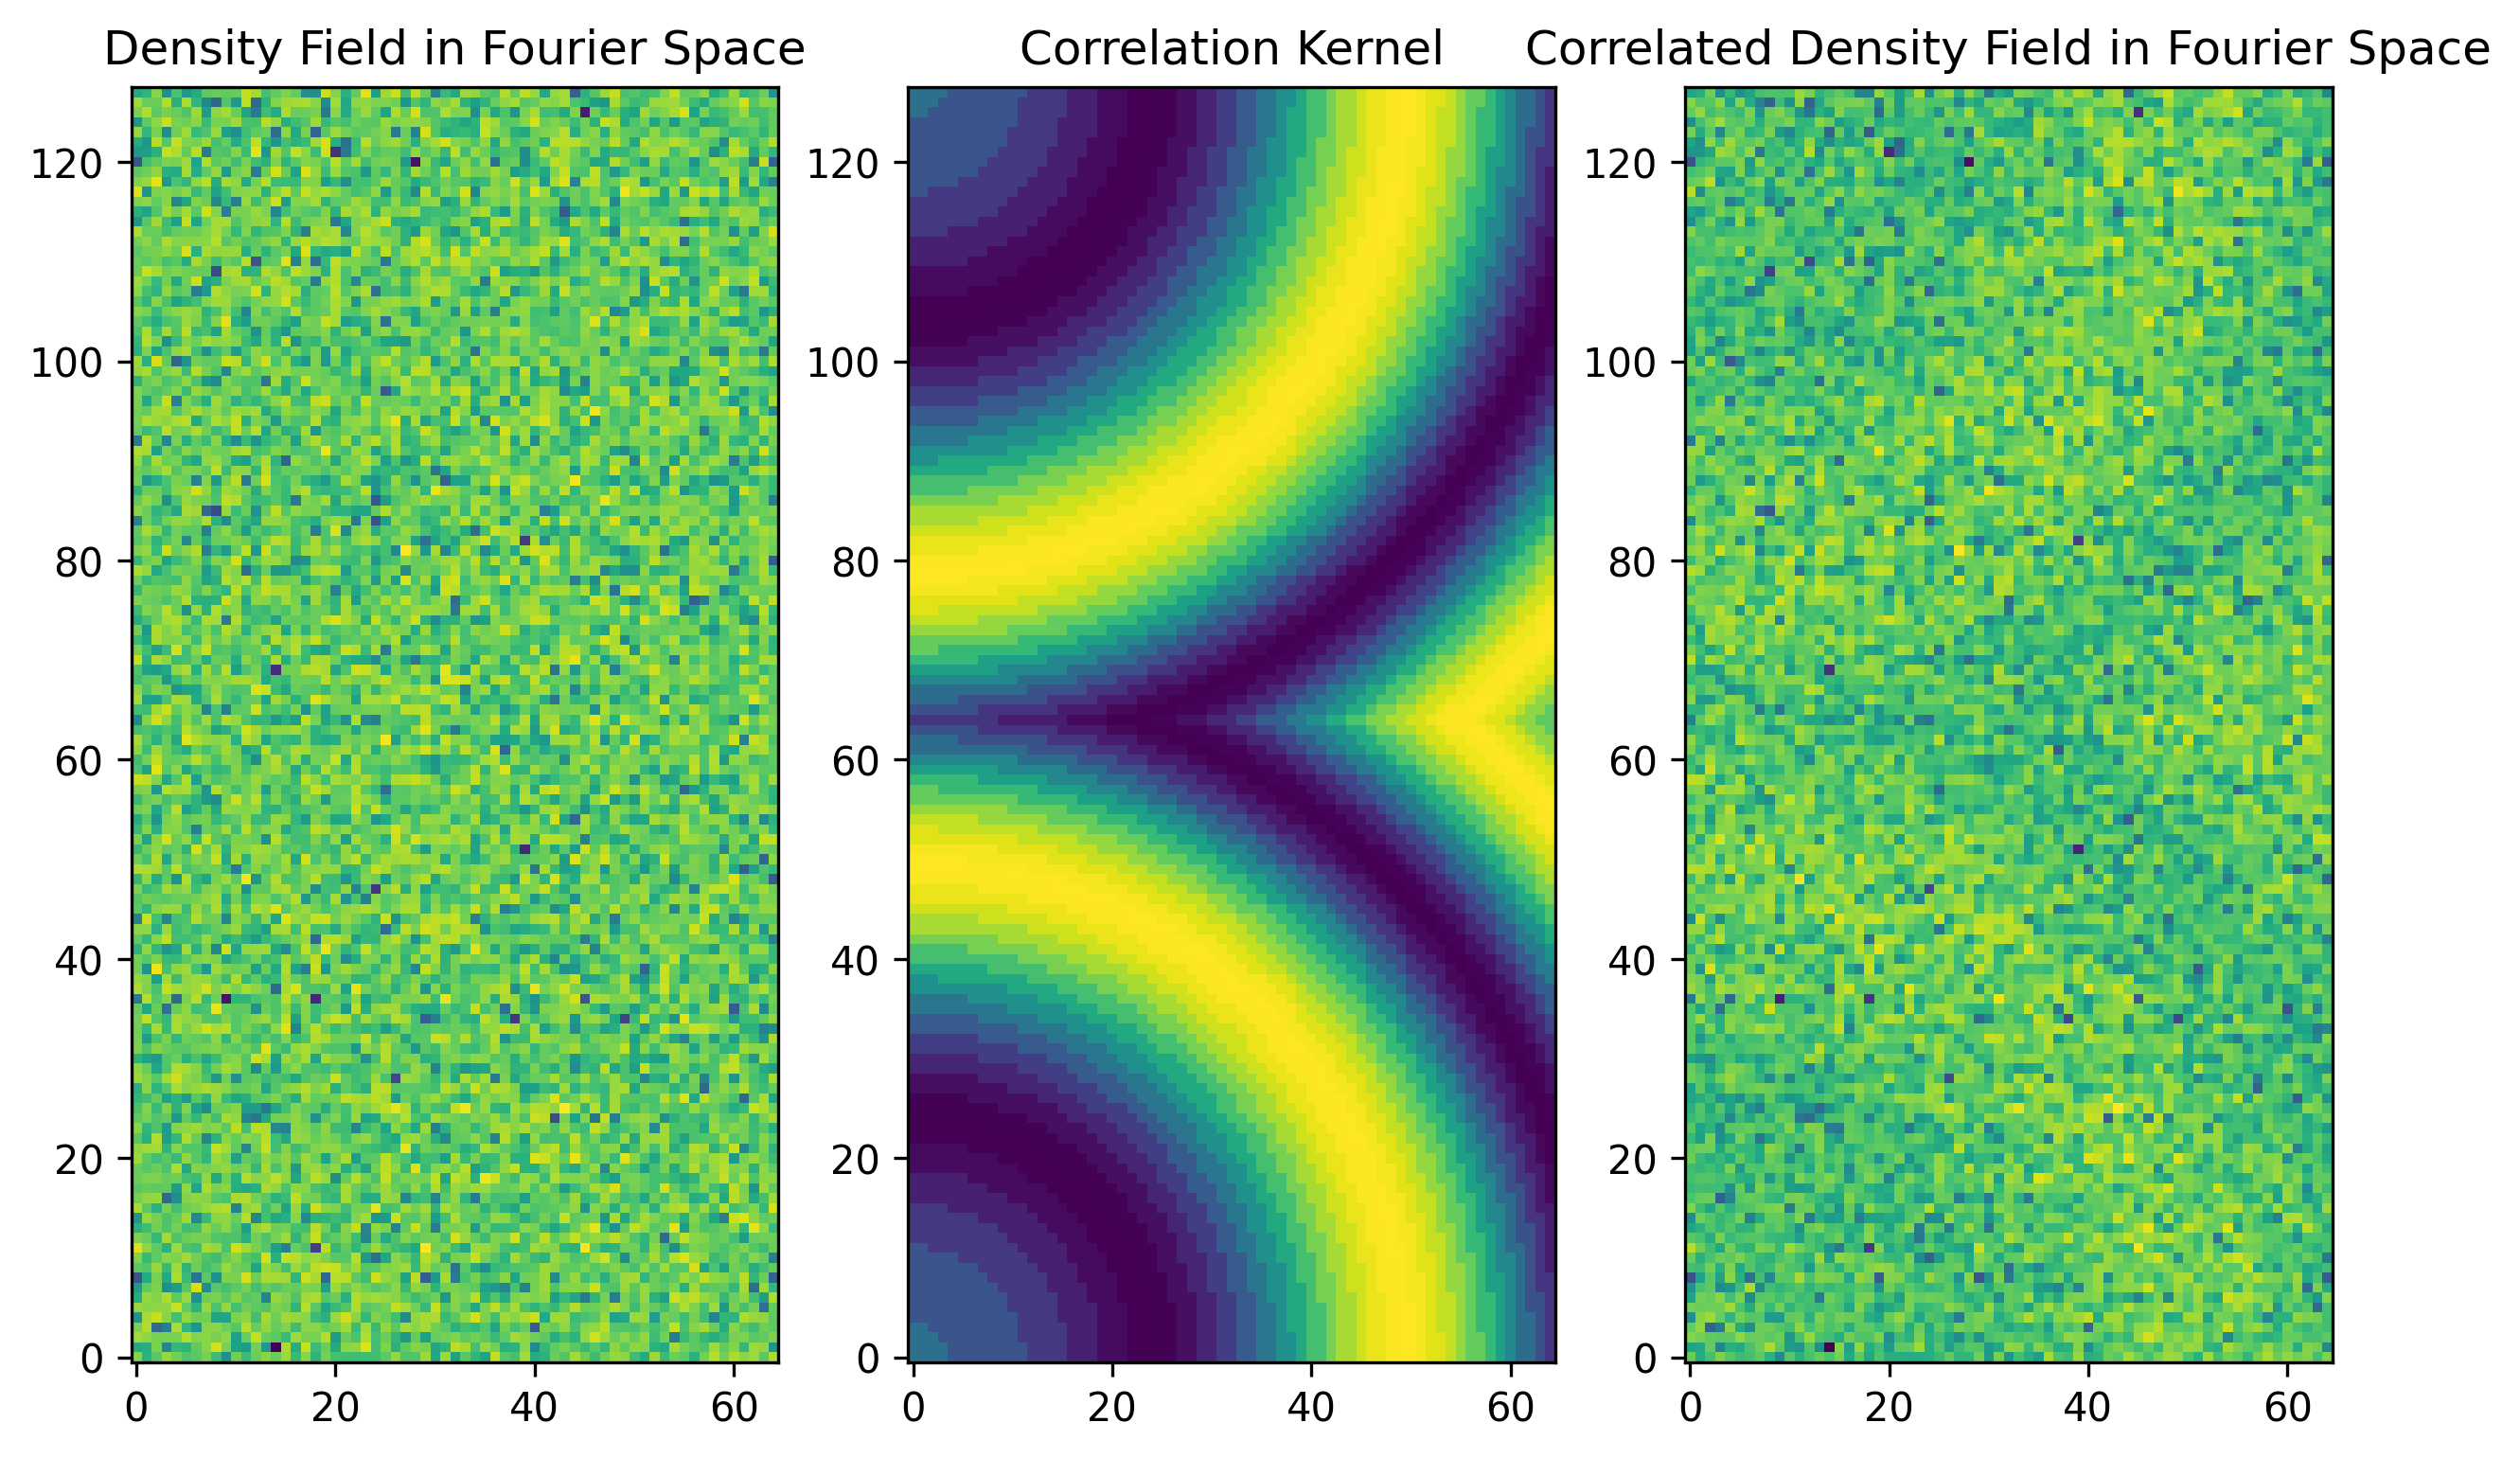
\includegraphics[width=0.7\linewidth]{img/IC_sine_corr.png}
   \caption{Random distribution, its power spectrum, and the desired power spectrum.}
\label{fig:cocrr}
\end{figure}

We then compute the Fourier transform of the white noise density field $\mathbf{W}$, apply the correlation kernel and transform it back to real space

\begin{equation}
     \rho(\mathbf{x}) = \mathcal{F}^{-1} \Bigl( \mathcal{F}(\mathbf{W})[\mathbf{k}] \cdot A(\mathbf{k}) \Bigr).
\end{equation}

We can see the resulting density field and its power spectrum in figure \ref{fig:result}.


\begin{figure}[h]
    \centering
    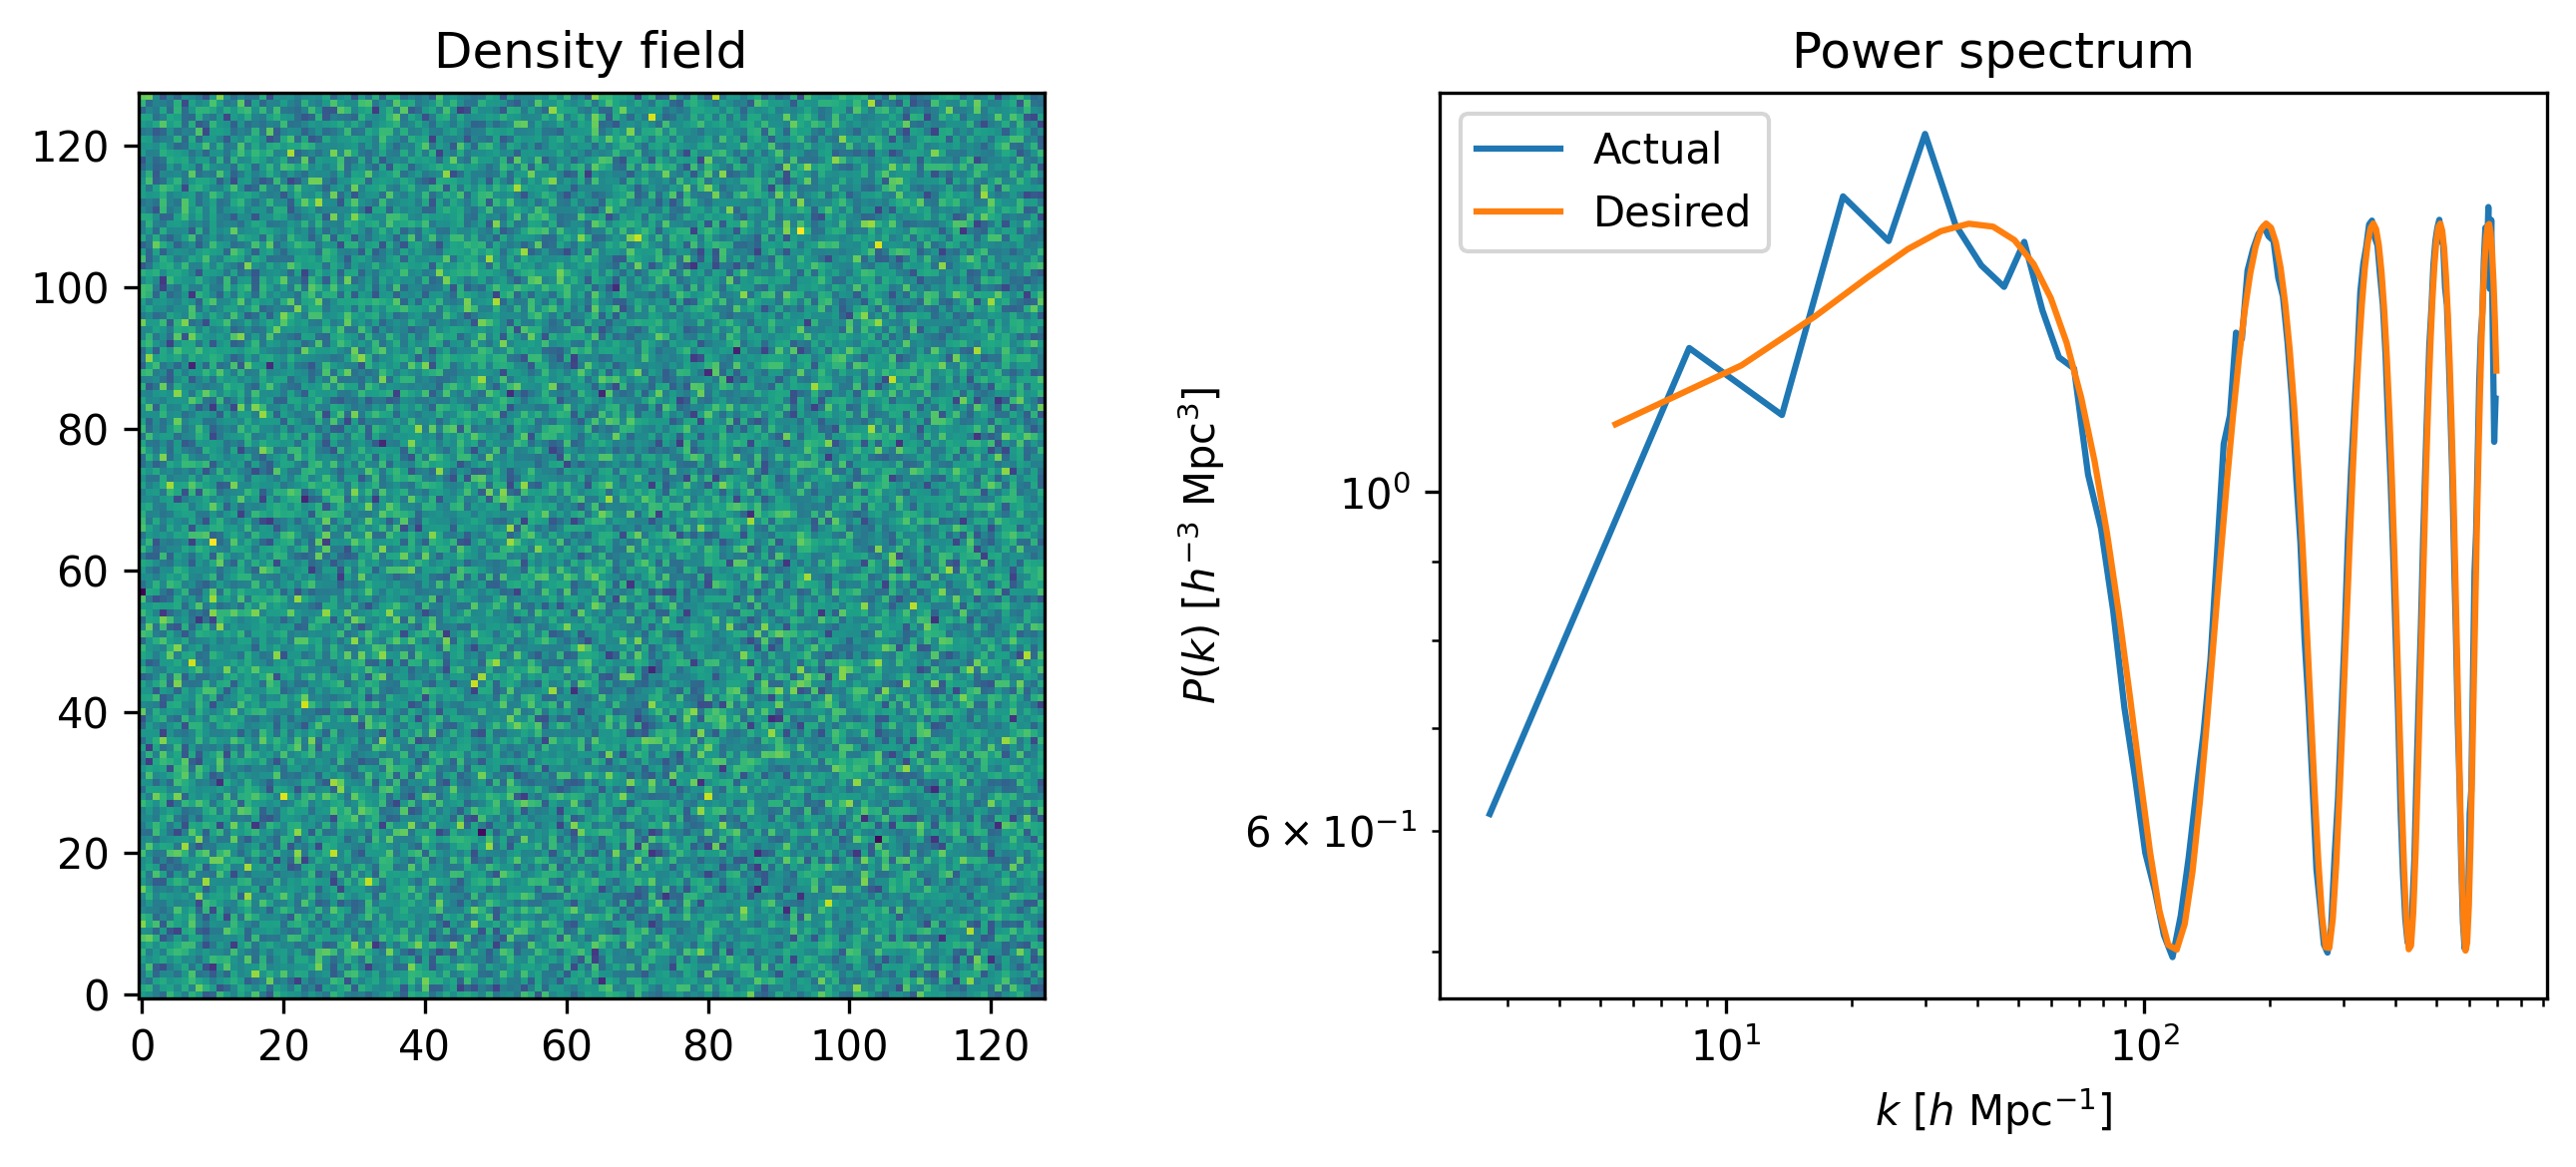
\includegraphics[width=0.7\linewidth]{img/IC_sine_res.png}
    \caption{The resulting density field, its power spectrum and the desired power spectrum.}
    \label{fig:result}
\end{figure}



\subsection{N-Body Simulations}
\label{nbody}

In this section, we briefly explore some ways to simulate the density field initial conditions forward in time using numerical solvers. N-body simulations are a fundamental tool in cosmology, used to model the gravitational dynamics of systems with many interacting particles. Various methods have been developed to tackle the computational challenges inherent in simulating such systems, which are aimed at bringing down the computational complexity of $N^2$ given for a naive implementation on $N$ particles.

\subsubsection{Particle Mesh Method}
\label{pm}
With the particle mesh method, we employ a discrete density field and unstructured particle density representations simultaneously. The positions of the unstructured particles $\mathbf{x}(i, t)$ and their masses $m(i)$ are assigned to the grid cells of a three-dimensional density grid $\rho$ using a mass assignment method as described in section \ref{mass-assignment}. Once a structured density field is obtained, we can solve for the gravitational potential on the field by solving the Poisson equation \ref{eq:potential-poisson}. We then read out the gravitational potential affecting each particle in the unstructured representation, by looking up the potential value on its position. More involved interpolation schemes can be used to interpolate the gravitational potential values over nearby grid cells.

The Poisson equation can be solved on a periodic density field, with the help of the Fast Fourier Transform (FFT), resulting in a runtime of $O(L \log L)$. Alternatively, a multi-grid method can be employed resulting in $O(L)$ time \citep{demmel1996solving, mccormick1987multigrid}, where $L$ is the grid size. The method is fast, but introduces an error which is inversely related to the grid resolution where the forces are evaluated on. Solving the potential on very high resolved grid, might be infeasible due to the required memory. Hence, the particle mesh method introduces an additional term in the computational and memory complexity, which is unrelated to the number of particles. This becomes especially problematic when we have highly dense regions, where the grid resolution assigns multiple particle masses on the same grid cell, resulting inaccurate force computations.

\subsubsection{Fast Multipole Method}
\label{fmm}

For accurate large-scale gravity simulations, methods derived from the Barnes-Hut approach offer a better alternative \citep{barnes1986hierarchical}. Barnes-Hut works by dividing the spatial domain into an octree, where each leaf node contains the same number of particles. The direct gravity is only computed for nearby particles, while particles that are farther apart are summarized as a single large particle, with its center of mass as its position. Alternatively, for higher accuracy, the multipole expansion can be used to more precisely represent a set of particles. The next evolution in this approach came with the implementation of the Fast Multipole Method (FMM) \citep{rokhlin1985rapid}, which, given a tolerance $\epsilon$, can compute all forces in an N-body system in $O(N \log \frac{1}{\epsilon})$ time. The FMM has been implemented in PKDGRAV3 to simulate trillions of particles \citep{potter2017pkdgrav3}.


\newpage
\newpage
\section{Neural Networks and Optimization}
\label{nno}

In this section, we provide a small recap over gradient-based optimization, automatic differentiation, convolutional neural networks, spectral convolutional neural networks and specific architectures. 
An in-depth understanding of optimization methods and automatic differentiations helps us understand existing approaches for IC predictions as well as their opportunities and challenges. Furtermore understanding the fundamentals of optimization is essential for any training of neural networks. Understand automatic differentiation, can be extremely helpful to understand the computational and memory complexity of neural network training. With IC predictions, we are pushing the boundaries of the available GPU memory. A theoretical understanding of the underlying computational methods can help us identify the bottlenecks and propose solutions.

\subsection{Gradient-Based Optimization}

We define a learnable function \(\mathbf{f}(\mathbf{x}, \theta) \colon \mathbb{R}^n \times \mathbb{R}^p \rightarrow \mathbb{R}^m\) that maps an input \(\mathbf{x}\) to an output \(\hat{\mathbf{y}}\), given parameters \(\theta\). The discrepancy between the ground truth \(\mathbf{y}\) and the prediction \(\hat{\mathbf{y}}\) should be minimal, and its magnitude is quantified by a scalar loss function \(L(\hat{\mathbf{y}}, \mathbf{y}) \colon \mathbb{R}^m \times \mathbb{R}^m \rightarrow \mathbb{R}\). 

An iterative gradient-based algorithm, works by gradually nudging the parameter vector $\theta$ in a direction, such that the loss $L$ is reduced, and the parameters are steered toward a satisfactory minimum. For given parameters, the loss is evaluated as $L(\mathbf{f}(\mathbf{x}, \theta), \mathbf{y})$, which we simply denote as $L$. Oftentimes, $\theta$ is initially sampled from a random distribution. However, oftentimes specific scaling factors are leveraged or more involved heuristics applied. The parameters are then iteratively improved by calculating the update vector $\nabla$ and determining a learning rate $r$. In each iteration, we update the learnable parameters with

\begin{equation}
    \theta_{i+1} = \theta_{i} + \nabla_i * r_i.
\end{equation}

There exists different strategies to compute $\nabla$, where the best convergence rate is achieved with the Gauss Newton algorithm \citep{thuerey2021physics}. The gauss Newton Algorithm requires a full computation of the Hessian, which then results in an update defined as

\begin{equation}
    \nabla = {\mathbf{H}_L}^{-1} \mathbf{J}_L^{T},
\end{equation}

where $\mathbf{J}$ is the Jacobin matrix defined as 

\begin{equation}
    \mathbf{J}_L = \begin{bmatrix}
        \frac{\partial L}{\theta_1} & \frac{\partial L}{\theta_2} & \dots &\frac{\partial L}{\theta_p}
    \end{bmatrix}
\end{equation}

and the Hessian $\mathbf{H}$

\begin{equation}
    \mathbf{H}_L = \begin{bmatrix}
        \frac{\partial^2 L}{\partial \theta_1^2} & \frac{\partial^2 L}{\partial \theta_1 \theta_2} & \dots & \frac{\partial^2 L}{\partial \theta_1 \theta_p} \\ 
        \frac{\partial^2 L}{\partial \theta_2 \theta 1} & \frac{\partial^2 L}{\partial \theta_2^2} & \dots & \frac{\partial^2 L}{\partial \theta_2 \theta_p} \\
        \vdots & \vdots & \ddots & \vdots \\ 
        \frac{\partial^2 L}{\partial \theta_p \theta 1} & \frac{\partial^2 L}{\partial \theta_p \theta 2} & \dots & \frac{\partial^2 L}{\partial \theta_p^2}
    \end{bmatrix}.
\end{equation}

A challenge with the Newton method is determining the Hessian matrix $\mathbf{H}_L$, as it represents the gradient of the gradient. In theory, both the Hessian and the Jacobian could be solved analytically; however, such large computations are error-prone and symbolic differentiation methods are computationally infeasible. Therefore, in large systems, the Jacobian and the Hessian need to be computed using automatic differentiation (AD). The computational complexity of finding the Jacobian with AD is equivalent to an evaluation of the function $F$, but finding the Hessian is $p$ times more complex, where $p$ denotes the number of parameters. This number can become huge, especially in neural networks, with language models reaching several billion parameters \citep{jiang2023mistral}. For this reason, various approximations to the Hessian matrix have been proposed, with arguably the most frequently used approach being the Adam optimizer \citep{kingma2014adam}, which provides a rough approximation of the Hessian \citep{thuerey2021physics}.

\begin{equation}
    \mathbf{H}_L \simeq \sqrt{\text{diag}(\mathbf{J}^T\mathbf{J})}.
\end{equation}

Note the above equation is not computed so explicitly, however various algorithmic tricks such as momentum are applied to Adam. Those tricks mimic the effects of the Hessian and can be approximated with the above equation. Due to the approximate nature, the computed gradient $\nabla$ is less precise, leading to a slower convergence. After all, the choice of the optimizer is a trade-off between the computing time of a single evaluation and the precision of the gradient, which in turn can influence the number of required optimization iterations \citep{bottou2007tradeoffs}. The preferred method to find the Jacobian and if necessary the hessian of a programmed function is automatic differentiation. It's flexible, accurate and involves little to no analytic skills to apply.

\subsection{Automatic Differentiation}
\label{ad}

To understand automatic differentiation, we take a more general function $\mathcal{F} \colon \mathbb{R}^n \rightarrow \mathbb{R}^m$, programmed in an arbitrary programming language. In this case, function consists of atomic operations, such as addition and multiplication and control statements. We denote its components as $\{f_1, f_2, \dots f_{k})$ where $F = f_{k} \circ \dots \circ f_2 \circ f_1$. The input of an atomic operator $f_i$ is organized in a vector as $\mathbf{x}_i \in \mathbf{R}^{s_i}$, whereas the output as $\mathbf{x}_{i_1} \in \mathbf{R}^{s_{i+1}}$. Hence, a function $f_i$ is of shape 

\begin{equation}
    f_i \colon \mathbb{R}^{s_i} \rightarrow \mathbb{R}^{s_{i+1}}
\end{equation}

and we can denote the dimensions of all variables as a set $\{s_1, s_2, \dots s_n, s_{k+1}$\}, where $s_1 = n$ and $s_{k+1} = m$. The whole program is executed as a composition of the atomic operators

\begin{equation}
    \mathbf{x}_{n+1} = f_k( \dots (f_2(f_1(\mathbf{x}_1)))
\end{equation} 

and a state $\mathbf{x}_{i}$ can be found with

\begin{equation}
    \mathbf{x}_{i} = f_{i-1}( \dots (f_2(f_1(\mathbf{x}_1))).
\end{equation}

In our case, we want to find the partial derivative $\frac{\partial \mathbf{x}_n}{\partial \mathbf{x}_1}$ which is the same as writing

\begin{equation}
    \frac{\partial \mathbf{x}_k}{\partial \mathbf{x}_1} = \frac{\partial f_k( \dots (f_2(f_1(\mathbf{x}_1)))}{\partial \mathbf{x}_1}.
\end{equation}

or by leveraging the chain rule

\begin{equation}
    \frac{\partial \mathbf{x}_{k+1}}{\partial \mathbf{x}_1} = \frac{\partial f_n(\mathbf{x}_{k})}{\partial \mathbf{x}_{k}} \dots \frac{\partial f_{2}(\mathbf{x}_2)}{\partial \mathbf{x}_{1}} \frac{\partial f_{1}(\mathbf{x}_1)}{\partial \mathbf{x}_1} = \frac{\partial \mathbf{x}_{k+1}}{\partial \mathbf{x}_{k}} \dots \frac{\partial \mathbf{x}_{3}}{\partial \mathbf{x}_{2}} \frac{\partial \mathbf{x}_{2}}{\partial \mathbf{x}_{1}}.
\end{equation}

Hence, if all partial derivatives of the atomic operations in a program are defined,  we can compute the derivatives using the chain rule using the forward recursive relationship

\begin{equation}
    \frac{\partial \mathbf{x}_{i+1}}{\partial \mathbf{x}_1} = \frac{\partial \mathbf{x}_{i}}{\partial \mathbf{x}_{i-1}} \cdot  \frac{\partial \mathbf{x}_{i-1}}{\partial \mathbf{x}_{1}},
\end{equation}

where we define the base case as the identity tensor

\begin{equation}
    \frac{\partial \mathbf{x}_{1}}{\partial \mathbf{x}_{1}} = \begin{bmatrix}
        1 & \dots & 1
    \end{bmatrix}.
\end{equation}

We can also leverage the backward recursion

\begin{equation}
    \frac{\partial \mathbf{x}_{k}}{\partial \mathbf{x}_i} = \frac{\partial \mathbf{x}_{k}}{\partial \mathbf{x}_{i+1}} \cdot  \frac{\partial \mathbf{x}_{i+1}}{\partial \mathbf{x}_{i}},
\end{equation}

where the base case is 

\begin{equation}
    \frac{\partial \mathbf{x}_{k}}{\partial \mathbf{x}_{k}} = \begin{bmatrix}
        1 & \dots & 1
    \end{bmatrix}.
\end{equation}

If we use the backward recursion, the automatic differentiation (AD) algorithm is commonly referred to as backward differentiation or reverse mode AD. Conversely, if we use the forward recursion, it is termed forward differentiation or forward mode AD. Both methods are mathematically equivalent but differ in computational and memory complexity. When performing AD, we can imagine the gradient vector being either pushed or pulled through the chain of evaluations. The final Jacobian, or gradient, has to be of shape $n \times m$ where $n$ is the number of inputs and $m$ the number of outputs. When we push (forward mode AD) the gradient from start to finish, one dimension of its shape has to be retained $n$ through the entire process. Vice versa for backward propagation, the size $m$ is pulled through the entire chain. The rule of thumb is, if $m$ is smaller than $n$ we should use backward mode AD and forward mode in all other cases. For applications in neural networks, the goal is to compute the derivative of the scalar loss function regarding all parameters of the neural network, hence $m$ is equal to one. This applies not only to the training of neural networks but all optimization problems. The problem with back-propagation is the direction of the gradient, which is the reverse of the primal evaluation of the chain of operations. Therefore, to compute the reverse mode AD, first all primary values need to be computed, memorized and then leveraged to get the gradients. Consequently, for each atomic operation, we need to store its inputs in memory. For large programs, for example large neural networks that are designed to be executed on the GPU, a large memory footprint can become a problem. 

\subsection{Discrete Convolutional Operator}

Many neural networks applied to grid-based data, such as images, videos, and finite difference simulations, leverage the discrete convolutional operator as an essential building block. Convolutions are flexible operations capable of implementing various transformations, such as sharpening, blurring, contrast enhancement, and calculating derivatives and gradients.

Consider two discrete functions, $u$ and $v$, where $u$ typically represents our quantity of interest and $v$ is the convolution operator. In the context of Convolutional Neural Networks (CNNs), we assume both the quantity of interest $u$ and the convolution operator $v$ are bounded. We define a bounded domain in three dimensions as $\Omega_k$

\begin{equation}
\label{eq:bounded-domain}
    \Omega_{a}^{b} = \{ \mathbf{x} \in \mathbb{Z}^3 \mid (\forall i \in \{1, 2, 3\}) [a \leq x_i \leq b] \}.
\end{equation}

Thus, we have \( u \colon \Omega_n \rightarrow \mathbb{R} \) and \( c \colon \Omega_k \rightarrow \mathbb{R} \). The discrete convolutional operator \(\ast\) is defined as

\begin{equation}
    (u \ast v)[\mathbf{x}] = \sum_{\mathbf{y} \in \Omega_{-k}^{k}} u[\mathbf{u} - \mathbf{y}] \cdot v[\mathbf{y}],
\end{equation}

where \(2k + 1\) represents the kernel size. Crucially, it is important to define the boundary conditions, as \(\mathbf{v} - \mathbf{x}\) can fall outside \(\Omega_n\). In our case, periodic boundary conditions suffice, so we abstain from discussing other conditions. We can define the boundary condition function as a vector modulo operation

\begin{equation}
    m(\mathbf{x}, n) = \begin{bmatrix}
        x_1 \mod n & x_2 \mod n & x_3 \mod n
    \end{bmatrix}
\end{equation}

and the convolution operator becomes 

\begin{equation}
    (u \ast v)[\mathbf{x}] = \sum_{\mathbf{y} \in \Omega_{-k}^{k}} u\left[m(\mathbf{x} - \mathbf{y}, n)\right] \cdot v[\mathbf{y}].
\end{equation}

Given the convolutional operator, we can define a convolutional layer, which is a generalization of discrete convolution operators with additional concepts. We define the number of input and output channels as $c_{in}$ and $c_{out}$, respectively, and adapt the operator definition

\begin{equation}
    (u \ast v)[\mathbf{x}, c] = \sum_{i \in \{0, \dots, c_{in}\}} \sum_{\mathbf{y} \in \Omega_{-k}^{k}} u\left[m(s \cdot \mathbf{v} - \mathbf{x}, n), i\right] \cdot v[\mathbf{y}, c, i].
\end{equation}

Further, we introduce a stride $s \in \mathbb{N}$. The output of the convolutional operator is evaluated only at every $s$ -th entry, thus reducing the output size by the stride factor. Given periodic boundary conditions, the output size $n_{out}$ of a convolutional layer with stride $s$ can be determined as

\begin{equation}
    n_{out} = \lfloor n_{in} / s \rfloor,
\end{equation}

where $n_{in}$ is the input size of a cubic 3D tensor. With periodic boundary conditions, the kernel size $k$ does not affect the output size, and no padding is required. The convolutional layer then becomes

\begin{equation}
    (u \ast v)[\mathbf{x}, c] = \sum_{i \in \{0, \dots, c_{in}\}} \sum_{\mathbf{y} \in \Omega_{-k}^{k}} u\left[m(s \cdot \mathbf{x} - \mathbf{y}, n), i\right] \cdot v[\mathbf{y}, c, i].
\end{equation}

In some cases, we may want the domain to become larger rather than smaller. This can be achieved by leveraging the transpose convolutional layer, where the relationship between input and output size is defined as:

\begin{equation}
    n_{out} = n_{in} \cdot s.
\end{equation}

The equation then becomes

\begin{equation}
    (u \ast v)[\mathbf{x}, c] = \sum_{i \in \{0, \dots, c_{in}\}} \sum_{\mathbf{y} \in \Omega_{-k}^{k}} u\left[m(\lfloor \mathbf{x} / s \rfloor - \mathbf{y}, n), i\right] \cdot v[\mathbf{y}, c, i].
\end{equation}

In convolutional neural networks (CNNs), the parameters of \(c\) are learned. The size of \(c\) is referred to as the kernel size. With convolutional layers, the number of parameters in the operator \(c\) remains constant, even as the size of our quantity of interest increases. Hence, the operator is invariant regarding the size of the domain. Convolutional neural networks (CNNs), which are essentially chains of convolutional layers, were formally introduced in 1998 \citep{lecun1998gradient} and have been highly successful in computer vision tasks, such as image classification \citep{krizhevsky2012imagenet}.

\subsection{UNet}

The U-Net is a specific architectural layout for a neural network, originally introduced for cell labeling tasks \citep{ronneberger2015u}, but often employed in various domains beyond biology. Recently, it has, has demonstrated promising results when integrated with an adversarial network to generate gas distributions predicated on dark matter distributions \citep{bernardini2022ember}.
The defining characteristic of the U-Net architecture is its U-shaped structure. This consists of two main segments: a contracting path (downsampling) and an expansive path (upsampling). During the downsampling phase, a series of convolutional layers are applied to progressively reduce the spatial dimensions of the input image while increasing the number of feature channels. This process results in a feature matrix with drastically altered dimensions. In the subsequent upsampling phase, transposed convolutional operators are utilized to restore the matrix back to its original dimensions. The advantage of U-Net lies in its ability to propagate information across the entire image due to this dimensionality transformation. Unlike a single convolutional layer, where the spread of information is constrained by the kernel size, the U-Net architecture enables broader contextual information transfer, which is crucial for accurate predictions across the entire input space. The original U-Net architecture, as proposed in the seminal paper, is visualized in Figure \ref{fig:unet}.
\begin{figure}[h]
    \centering
    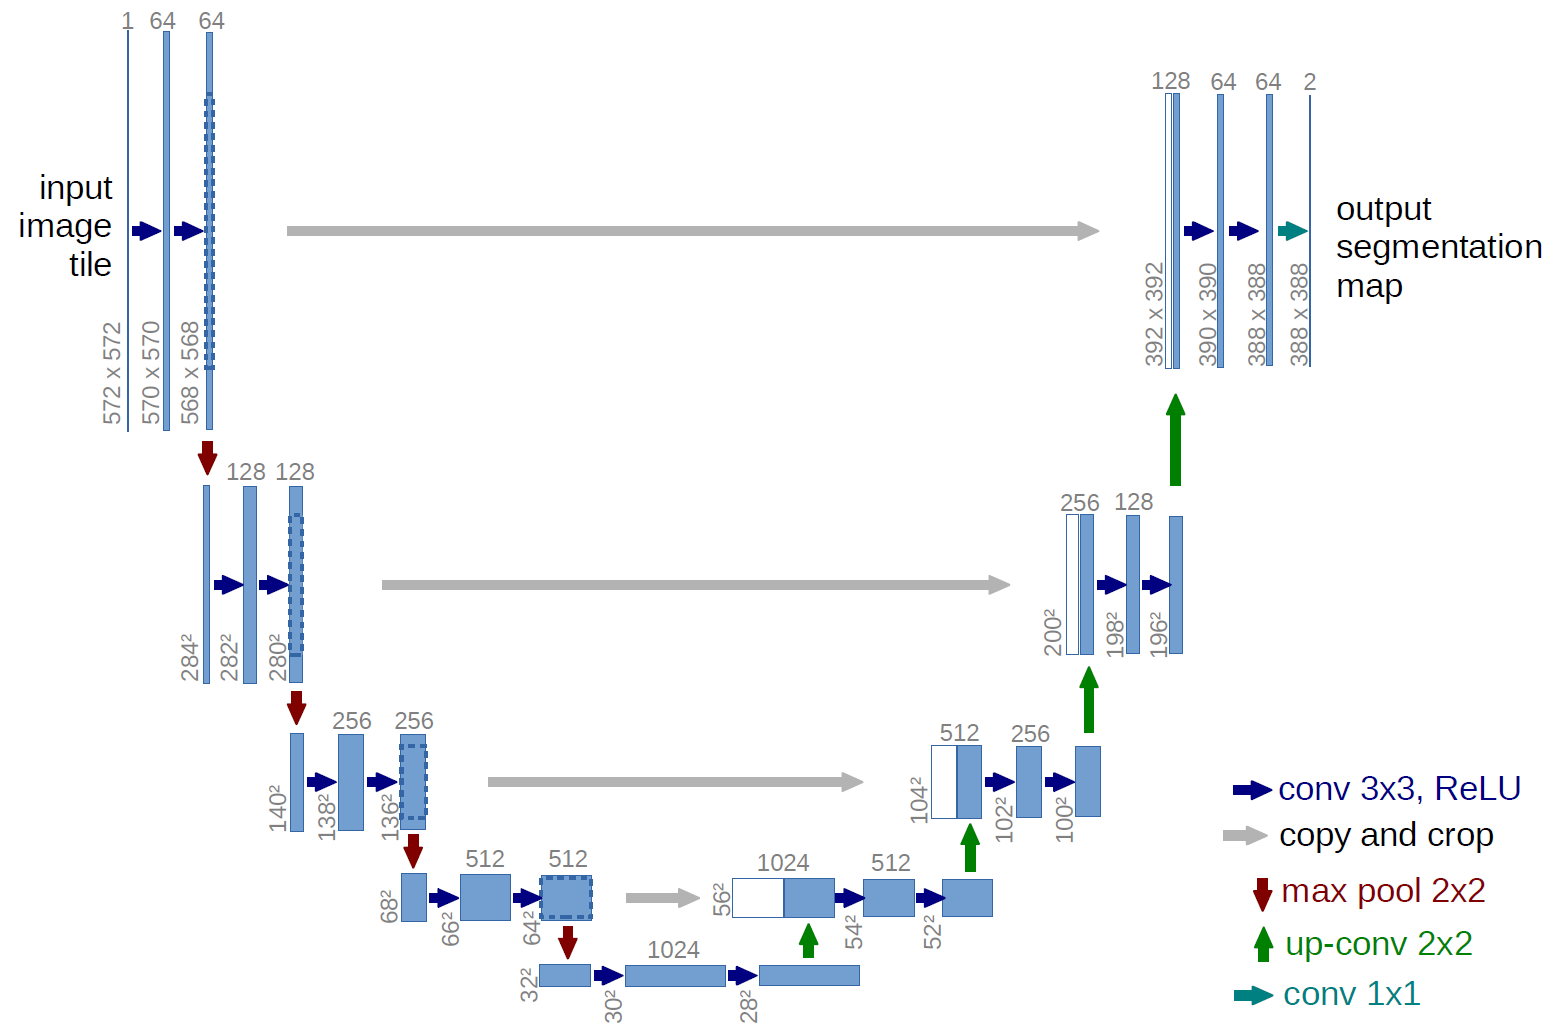
\includegraphics[width=0.8\linewidth]{img/unet.png}
    \caption{Architecture of the original UNet as proposed by \cite{ronneberger2015u}. A maxpooling layer, is a convolutional layer with a stride, which in this case is always two. An up.conv layer is a transposed convolutional layer with stride 2. }
    \label{fig:unet}
\end{figure}
    
\subsection{Spectral Convolution}
In the realm of physics-informed neural networks (PINNs) and physics-based deep learning, a frequent task is to develop surrogate models for solving partial differential equations (PDEs). The motivation behind this task is to create neural networks capable of solving PDEs faster or more precisely than traditional numerical solvers \citep{mcgreivy2024weak}. Fourier Neural Operators (FNOs) propose a formulation to learn a general solver for parameterized PDEs more efficiently than traditional architectures. The main idea is to define the parameters of the convolutional operator in Fourier space instead of real space \citep{li2020fourier}. Recall the discrete convolution for a single channel, for now, omitting periodic boundary conditions

\begin{equation}
    (u \ast v)[\mathbf{x}] = \sum_{\mathbf{y} \in \Omega_{-k, k}} u[\mathbf{x} - \mathbf{y}] \cdot v[\mathbf{y}].
\end{equation}

If we apply the periodic boundary conditions and the convolution theorem, the discrete convolution can be rewritten as

\begin{equation}
    \mathcal{F}(u \ast v)[\mathbf{k}] = \mathcal{F}(u)[\mathbf{k}] \cdot \mathcal{F}(v)[\mathbf{k}].
\end{equation}

Here, $\mathcal{F}$ denotes the discrete Fourier transform as defined by 

\begin{equation}
    \mathcal{F}(u)[\mathbf{k}] = \sum_{\mathbf{v} \in \Omega} u[\mathbf{v}] \, e^{-i2\pi \langle \mathbf{k}, \mathbf{v} \rangle},
\end{equation}

and $\mathcal{F}^{-1}$ denotes the inverse Fourier transform as 

\begin{equation}
    \mathcal{F}^{-1}(u)[\mathbf{v}] = \frac{1}{|\Omega|} \sum_{\mathbf{k} \in \hat{\Omega}} u[\mathbf{k}] \, e^{i2\pi \langle \mathbf{k}, \mathbf{v} \rangle}.
\end{equation}

Applying the inverse discrete Fourier transform \(\mathcal{F}^{-1}\) to both sides, we obtain

\begin{equation}
    (u \ast v)[\mathbf{x}] = \mathcal{F}^{-1}\Bigl(\mathcal{F}(u)[\mathbf{k}] \cdot \mathcal{F}(v)[\mathbf{k}]\Bigr).
\end{equation}

The FNO approach proposes parameterizing one of the convolutions — in this case, $v$ — in Fourier space. Thus, we introduce a learnable complex matrix $\mathbf{V} \in \mathbb{C}^3$. The convolution then becomes

\begin{equation}
    (u \ast v)[\mathbf{x}] = \mathcal{F}^{-1}\Bigl(\mathcal{F}(u)[\mathbf{k}] \cdot \mathbf{V}[\mathbf{k}] \Bigr).
\end{equation}

Just as we did for the normal convolution, we define the number of input channels as $c_{in}$. We then define the spectral convolution on a field with multiple channels as 

\begin{equation}
    (u \ast c)[\mathbf{v}, c] = \sum_{i \in \{0, \dots, c_{in}\}} \mathcal{F}^{-1}\Bigl(\mathcal{F}(u)[\mathbf{k}, i] \cdot \mathbf{V}[\mathbf{k}, c, i] \Bigr).
\end{equation}

This also means the learnable weight matrix becomes $\mathbf{V} \in \mathbb{C}^5$. By reducing the size of the learnable matrix \(\mathbf{G}\), we can apply the convolution to a specific set of wavelengths. This allows for more efficient and targeted operations within a defined frequency range. One significant advantage of this formulation is its computational efficiency: the fast Fourier transform has a complexity of \(O(N \log N)\), while the element-wise multiplication is \(O(N^2)\). In contrast, performing the same convolution in real space has a complexity of \(O(N^4)\). Another key benefit of this approach is the ability to restrict the convolution to a specified frequency range, meaning computational and memory resources can be directed towards larger structures, which are oftentimes more crucial in dynamical systems.

\subsection{FNO Architecture}


\begin{figure}[h]
    \centering
    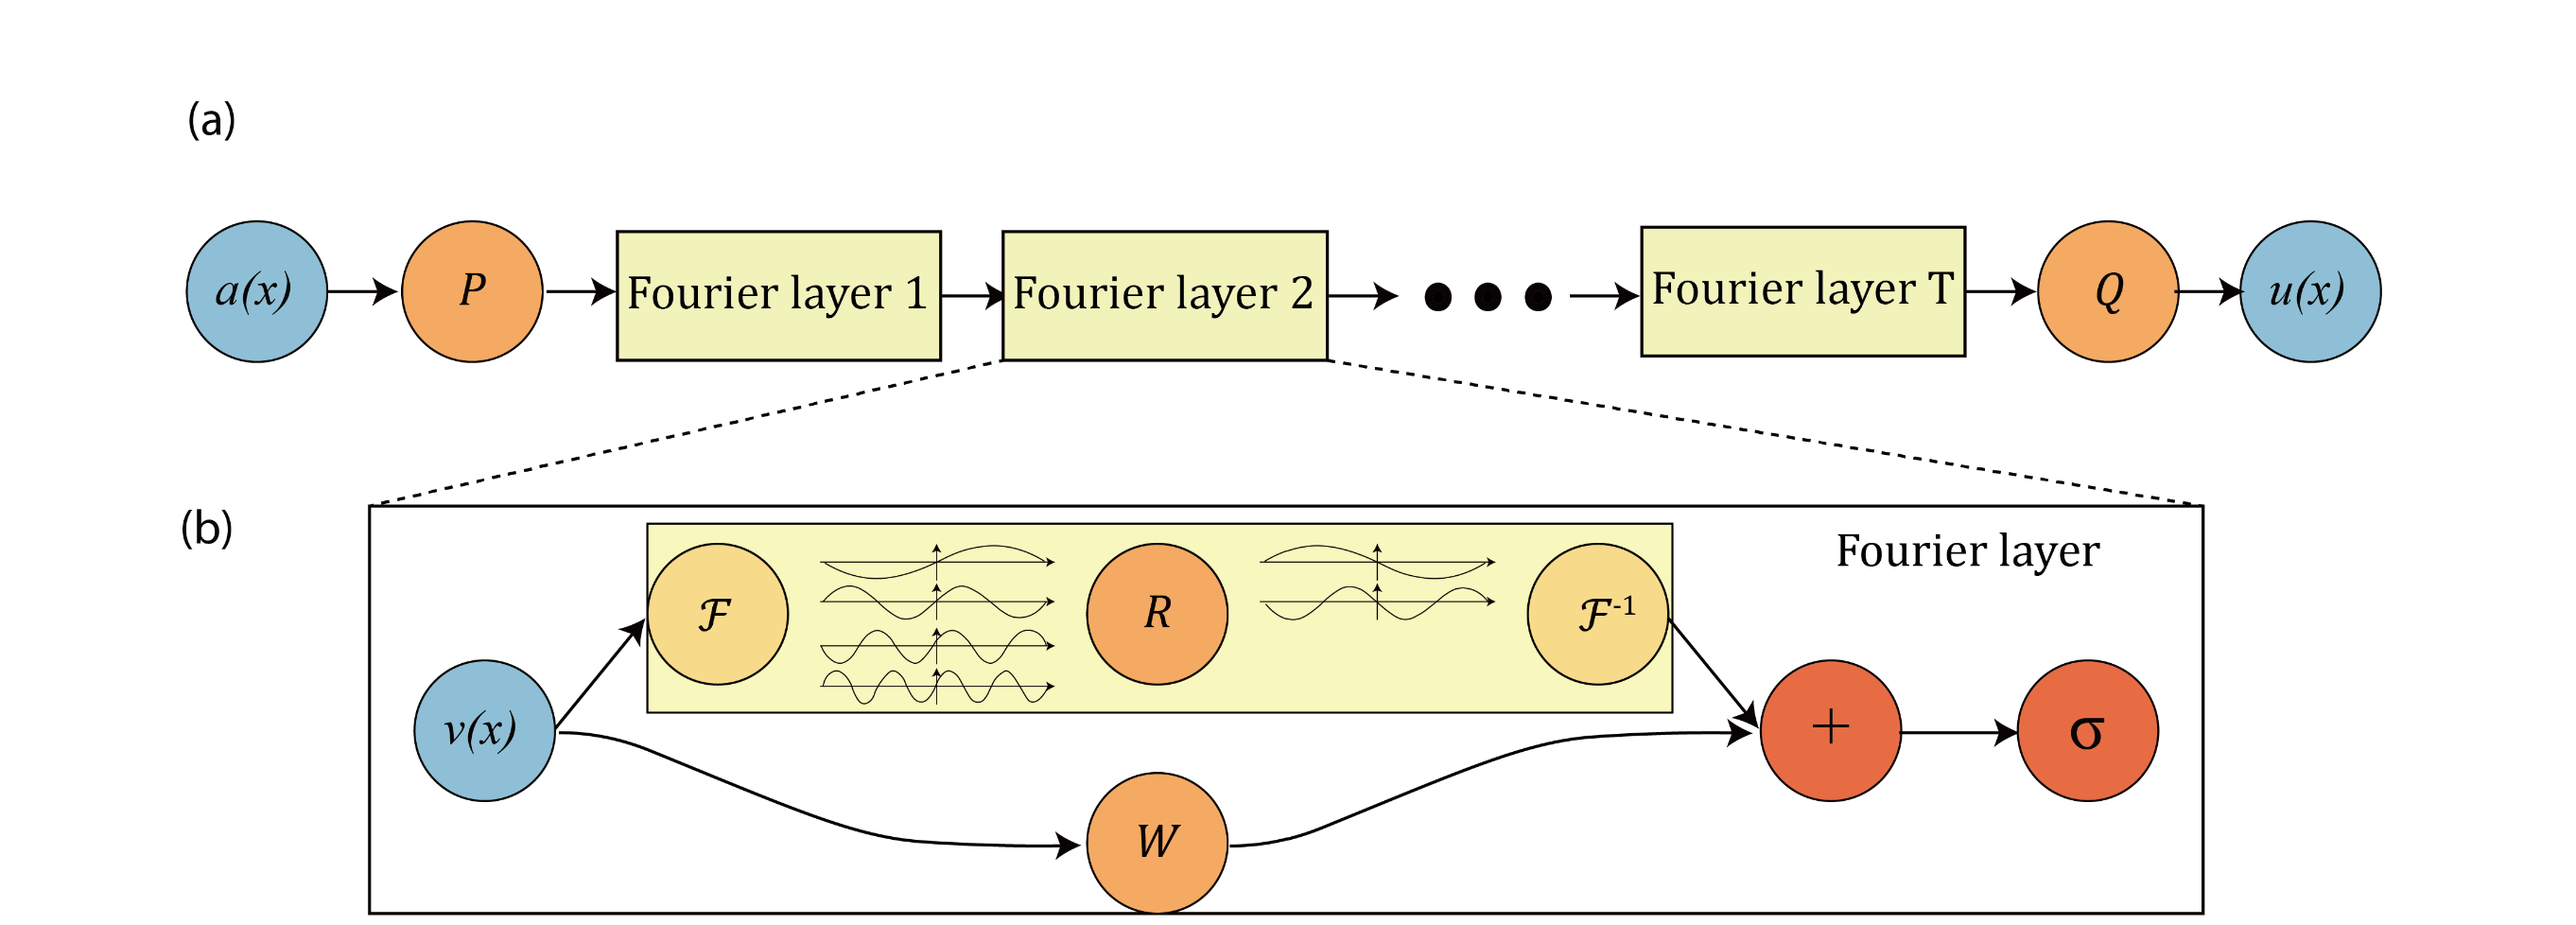
\includegraphics[width=0.9\linewidth]{img/Screenshot 2024-09-22 062730.png}
    \caption{(a) The entire Fourier Neural Operator architecture, (b) The Fourier Layer architecture. Image sourced from \cite{li2020fourier}.}
    \label{fig:fno-architecture}
\end{figure}

The FNO architecture \citep{li2020fourier} extends the concept of spectral convolution with the convolutional kernel defined in Fourier space. A Fourier layer first transforms the input into Fourier space, applies the complex convolution kernel $R$ to the lowest $k$ modes, and then uses the inverse Fourier transform to map the tensor back into real space. As seen in Figure \ref{fig:fno-architecture}, the input of each Fourier layer takes a second path, known as the bypass. The bypass path is visible at the bottom of the figure as it passes through the node marked as $W$. Here, a standard convolutional operator with a stride of one and a kernel size of one is applied. This effectively results in an element-wise matrix multiplication, where the size of the matrix is the square of the number of input channels. Then, the bypass is added to the convolved signal, and an activation function is applied. The full FNO includes several FNO layers, each having its own unique learnable parameters for $R$ and $W$. Finally, before and after the convolution, a lifting and projection convolution is applied. The lifting increases the input signal channels to the desired number of hidden channels, while the projection convolution reduces them in the opposite direction. 
The FNO architecture provides a good foundation for surrogate models aiming to replace or enhance traditional numerical solvers. The architecture outperforms UNet's and other competing architectures on difficult prediction tasks \citep{koehler2024apebench}.



% \begin{equation}
%     \mathbf{X}(k_0, k_1, k_2) = \frac{1}{L^3} \sum_{k_0=0}^{L-1} \sum_{k_1=0}^{L-1} \sum_{k_2=0}^{L-1} x(k_0, k_1, k_2) e^{i k_0 x_0 + k_1 x_1 + k_2 x_2},
% \end{equation}

% which we can rewrite in compact form as 

% \begin{equation}
%     \mathbf{X}(\mathbf{k}) = \frac{1}{L^3} \sum_{k_0=0}^{L-1} \sum_{k_1=0}^{L-1} \sum_{k_2=0}^{L-1} x(k_0, k_1, k_2) e^{i k_0 x_0 + k_1 x_1 + k_2 x_2},
% \end{equation}


\newpage
\section{Problem Statement and Related Work}

Our goal is to find constrained initial conditions for dark matter simulations. In cosmology, there exists various methods  to generate such constrained IC's. For constrained IC's generation processes, the goal is not to predict the IC with absolute accuracy. In fact, if such a thing was possible, it could be used as a reverse time integration method and we could simply predict the density state back in time, instead of predicting IC's and feeding them into numerical simulations. More important is to get the large-scale structures correct, which is oftentimes enough to seed the simulations that result in the desired final density state \citep{jasche2013bayesian}. Before diving deeper into related works in the realm of constrained initial conditions, we give a precise problem definition and explore the possibility of using reverse time integration to directly integrate back in time.

\subsection{Inverse Problem}
For a sequence of $n$ time steps, we are given a set of $N$ particles, each associated with a position and a mass. Hence, we have the positions $\mathbf{x}(i, t) \colon \mathbb{N} \times \mathbb{N} \rightarrow \mathbb{R}^3$ and the masses $m(i) \colon \mathbb{N} \times \mathbb{N} \rightarrow \mathbb{R}$ which are constant in time. In our case, the ground truth is sourced from simulation data generated by PKDGRAV3. We formulate the classical forward problem as

\begin{equation}
    \mathcal{P}_{n-1}\biggl( \dots \mathcal{P}_2\Bigl(\mathcal{P}_1\bigl(\mathbf{x}(i, t_{0})\bigr)\Bigr)\biggr) \approx \mathbf{x}(i, t_{n}),
\end{equation}

where $\mathcal{P}_i$ could be a single step of PKDGRAV3. Our primary goal is to find a function $\mathbf{g}$, which is capable of predicting the initial state of the particle distribution, given their final distribution. The predicted initial state should result in a equivalent final state when fed into the forward solver. We can formulate this as an equation
 
\begin{equation}
    \mathcal{P}_{n-1}\biggl( \dots \mathcal{P}_2\Bigl(\mathcal{P}_1\bigl(\mathbf{g}(\mathbf{x}(i, t_{n}))\bigr)\Bigr)\biggr) \approx \mathbf{x}(i, t_{n}).
\end{equation}

To formulate the above into an objective function, the prediction $\mathbf{x}(i, t_{n}))$ needs to be fed back intro the forward solver. Because we don't have a differentiable version of PKDGRAV3, we cannot compute the gradient of an objective function which is based on the above goal. Hence, we formulate the weaker goal

\begin{equation}
    \mathbf{g}(\mathbf{x}(i, t_{n})) \approx \mathbf{x}(i, t_{0}),
\end{equation}

which we can formulate as a differentiable objective function. Once we have optimized the above, we can still test our solution using an objective function based on the stronger goal formulation. In section \ref{mass-assignment}, we have described the common CIC mass assignment, which maps particles to a density field. A procedure to map from a density field to particles, has to the best of our knowledge not been described in literature. We will propose an approach in section \ref{inverse-map}, but for now, we assume a bijective map does exist. Therefore, if we define a density field $\rho(\mathbf{y}, t) \colon \mathcal{S}_{L} \times \mathbb{N} \rightarrow \mathbb{R}$, where

\begin{equation}
    \mathcal{S}_{L} = \{ \mathbf{y} \in \mathbb{Z}^3 | (\forall i \in \{1, 2, 3\}) [0 \leq t_i \leq L] \}
\end{equation} 

and $L$ denotes the grid size. Given the bijective map, our goal is equivalent to finding a function $\mathbf{g}$, such that

\begin{equation}
    \mathbf{f}(\rho(\mathbf{y}, t_{n})) \approx \rho(\mathbf{y}, t_{0}).
\end{equation}

Working with the density grid $\rho$ allows us to use efficient and established neural network architectures, which are commonly applied in tasks based on finite difference numerical solvers. Working with particles, we would have to rely on graph-based architectures, which is a more novel field of research and arguably introduces further complexity. Therefore, we model the function $\mathbf{f}$ using an artificial neural network, where its parameters are optimized using gradient descent.

Before describing our method in detail, we dive into some alternative methods on how to solve the problem along with their challenges. 

\subsection{Reverse Time Integration}
 
In theory, if $\mathcal{P}_i^{-1}$ can be found, we could solve the problem as follows

\begin{equation}
    \mathcal{P}_{1}^{-1} \biggl( \dots \mathcal{P}_{n-2}^{-1}\Bigl(\mathcal{P}_{n-1}^{-1}\bigl(\mathbf{x}(i, t_{n})\bigr)\Bigr)\biggr) \approx \mathbf{x}(i, t_{0}).
\end{equation}

Here $\mathbf{f}$ would be equal to 

\begin{equation}
    \mathbf{f} = \mathcal{P}_{n-1}^{-1} \circ \dots \circ \mathcal{P}_1^{-1}
\end{equation}.

In practice, however, the method forward solver suffers from errors introduced in the discretization method and due to the finite numerical precision and oftentimes cannot be inverted perfectly. Many interesting processes are subject to non-linear dynamics, hence chaos theory does apply, and small inconsistencies can produce very different results. Therefore, instead of relying on $\mathcal{P}^{-1}$, we are forced to rely on different approaches. This is especially problematic for large simulations, as the error increases with the number of variables, time steps size and number of time steps as seen in figure \ref{fig:error_inverse}.

\begin{figure}
    \centering
    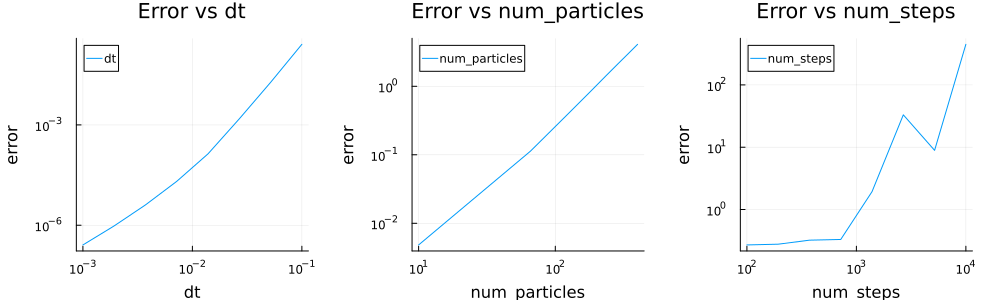
\includegraphics[width=0.8\linewidth]{img/error.png}
    \caption{Exploration of error in reverse time integration for N-Body system. The particles are integrated forwards in time using the leap frog integration scheme followed by a reverse time integration, also with leap frog integration but reversed forces. The error measures the mean of the squared defects between the particle's initial positions and their final positions after forwards and backwards integration. Parameters, if not declared otherwise in the plot are, $\Delta t= 0.1$ , $N = 100$, $n = 100$. The gravity forces are evaluated directly without any optimization, leveraging a brute force $O(N^2)$ approach. The simulation was done in a cubic periodic box of length one with a random, uniform initial particle distribution. To smoothen to avoid highly non-linear forces, a softening length of 0.01 was used. A more detailed description of the code can be found in section \ref{rev-integration}.}
    \label{fig:error_inverse}
\end{figure}

Reverse integrating the particle though time to recover the initial conditions, has been attempted \citep{nusser1992tracing} however it is hindered by numerical inaccuracies which appear during the reverse time integration, as well as incomplete observation data, making the data not feasible for real-world applications \citep{jasche2013bayesian}.

\subsection{Differentiable Solver for IC Optimization}
\label{IC-opt}

If we have a solver $\mathcal{P}$ and we can obtain its derivatives with respect to initial states (Hence a differentiable Solver) the task could be solver without finding a prediction function $\mathbf{f}$. Instead, we can directly solve the optimization problem

\begin{equation}
    L = \sum_{i \in 1 \dots N} \Biggl(\mathcal{P}_{n-1}\biggl( \dots \mathcal{P}_2\Bigl(\mathcal{P}_1\bigl(\rho(i, t_{0})\bigr)\Bigr)\biggr) - \rho(i, t_n)\Biggr)^2.
\end{equation}

Here we can leverage a gradient-based optimization method such as gradient descent or Adam can be leveraged to gradually improve the initial guess using the gradient

\begin{equation}
    \nabla L = \frac{L}{d \mathbf{u}(\mathbf{x}, 0)}.
\end{equation}

The gradient can be found via automatic differentiation as described in section \ref{ad}. At the time of writing this thesis, to our best knowledge, there exists only one differentiable N-Body solver used for gradient-based optimization of initial conditions \citep{li2024differentiable}. Other solvers, such as euclid where differentiable PMWD is implemented in pure python and cannot parallelize to a multi node computing system, hence its application is limited to small N-Body simulations. Furthermore, it is a particle mesh method based code, which relies on a spectral mode using FFT's to solve for the potential. Hence, the precision of the force evaluations is limited by the grid resolution and a single evaluation is in $O(N \log N)$, a number which could be reduced to $O(N)$ using the multi-grid method \citep{mccormick1987multigrid}. For large-scale analysis, it would be better to adapt an existing N-Body code such as PKDGRAV3 \citep{potter2017pkdgrav3}, which computes the forces using the efficient multipole expansion which lies in $O(N)$, to be  differentiable. However, in the case of PKDGRAV3, which has been written in C++ with custom CUDA Kernels, either the entire code needs to be adapted to work with a C++ AD library such as Enzyme or written in Julia or Python with more developed AD ecosystems. As documented in \ref{diff-julia}, our experience has shows how correctly applying Enzyme, is rather challenging and is a not feasible solution for this thesis. And even if the entire program is differentiable, there is still a problem as PKDGRAV3 operates on the very limit of the available memory. When differentiation over an entire forward solver using back propagation, we need to store the entire system state for each iteration to obtain the gradient. This means the memory footprint is defined as $n$ (the number of time steps) times the quantities of interest times the operations of int the numerical solver. The quantities of interest, are in the case of a particle-based method such as PKDGRAV3, the number of particles $N$ times its degrees of freedom. The factor can be reduced by leveraging check pointing \citep{wang2009minimal}, where with a recursive check-pointing scheme $\sqrt n$ states with even spacing are stored. The intermediate steps then need to be recomputed, introducing additional computing overhead of  $\sqrt n$. Finding an optimal schedule for a given memory capacity is a complex optimization problems itself, which can be solved with the Revolve algorithm \citep{griewank2000algorithm}. Lastly, the optimization process needs to be rerun for every initial condition we want to predict. Hence, if no check pointing is applied, the runtime can be approximated by $O(n N l)$, where $l$ denotes the number of iteration steps. If check pointing is applied, this increases to $O(\sqrt{n} n N l)$. In the case of PMWD, the default number of iteration steps $l$ is 1000.


\subsection{Statistical Methods for Constrained IC's}

Apart from leveraging differentiable physics and deep learning, various statistical approaches have been developed to generate constrained initial conditions for dark matter simulations. These methods utilize the full forward N-body model to iteratively refine initial guesses for the ICs based on observational data. By modeling the prior cosmological conditions alongside the physics governing large-scale structure formation, these statistical techniques aim to produce ICs, which lead to final states that are consistent with present-day observations when evolved over time \citep{jasche2013bayesian, kitaura2013initial}.

One prominent statistical method employed in this domain is the Bayesian approach \citep{jasche2013bayesian}, which provides a framework for incorporating prior information and observational data to constrain the initial conditions. Bayesian inference allows for a probabilistic interpretation of the ICs, where the likelihood of different initial states is updated iteratively using data from forward simulations. This iterative refinement process continues until the simulations closely match current observations, achieving convergence towards the most probable ICs.

These statistical models, however, come with certain drawbacks. Similarly to optimization with differentiable simulators, in each optimization step, the entire forward simulation needs to be executed. Furthermore, these approaches often involve complex inversion processes that are not fully understood in a theoretical sense but are optimized individually for each specific case. This lack of generalization limits their applicability to new scenarios without significant re-calibration.

In summary, while statistical methods offer a robust way to incorporate observational constraints into IC generation for dark matter simulations, they share some computational challenges associated with differentiable physics methods. Each iterative step requires substantial computational resources, and the inversion problem remains specific rather than universally applicable. Nonetheless, these techniques provide valuable insights into the structure formation in the universe by aligning simulation outcomes closely with observed data.



\subsection{Surrogate Model for IC Optimizationl}

Alternatively, we can train a surrogate model $\hat{\mathcal{P}}$, which is capable of approximating the true solver $\mathcal{P}$ with a sufficient accuracy. Surrogate models have been successfully applied in hydro dynamics \citep{asher2015review}, engineering \citep{forrester2008engineering} and chemistry \citep{kadupitiya2020machine}. In its basic version the surrogate models are used to replace forward models for increased performance or in some cases also improved accuracy \citep{mcgreivy2024weak}. More recently, the term Operator Learning has become the forefront of research in the realm of Physics Inspired Neural Network. The Operators, are designed to learn the numerical schemes required in specific problem domains, which could for example be the solution to a specific PDE. The operators have been applied in many domains such as weather forecasting \citep{pathak2022fourcastnet} and engineering design \citep{liu2023deepoheat}. Most recent research is based on the specific Fourier Neural Operator design \citep{li2020fourier} or adaptations of it \citep{long2024invertible}. 

All neural networks are inherently differentiable and subsequently also the described surrogate models and operators. Therefore, the learned networks, if capable of predicting the forward problem, can be leveraged to optimize the initial conditions. At the time of the writing of this thesis, to the best of our knowledge, there exists no attempt at creating a surrogate forward model capable of predictions across time in cosmological N-Body simulations. Forward surrogate models combined with gradient-based optimization have been used frequently in geometry optimizations for airplanes \citep{mack2007surrogate}. By quantifying the aerodynamics qualities of an aircraft structure with a loss function defined, the geometry can be optimized by propagating the loss through the surrogate forward aerodynamic model. Successful examples of this technique are rare due to several reasons, the surrogate model oftentimes yields gradients which are less accurate than the actual forward simulations \citep{forrester2009recent}. 

If we can find a model $\hat{\mathcal{P}}$, which is capable of approximating the true solver $\mathcal{P}$, we can leverage the same technique which has been described in section \ref{IC-opt}, where we replace the simulation model with the surrogate model. Effectively, the optimization becomes

\begin{equation}
    L = \sum_{i \in 1 \dots N} \Biggl(\hat{\mathcal{P}}_{n-1}\biggl( \dots \hat{\mathcal{P}}_2\Bigl(\hat{\mathcal{P}}_1\bigl(\rho(i, t_{0})\bigr)\Bigr)\biggr) - \rho(i, t_n)\Biggr)^2.
\end{equation}

There are three motivations to leverage a surrogate model instead of the simulation model to optimize the initial conditions. (1) The surrogate model might be a lot faster than the simulation, hence overall improving the speed of the optimization process. (2) Implementing a differentiable version of the simulation code is not feasible due to time constraints. (3) the surrogate model might be based on real data, where an accurate the simulation is unknown. In our case, the motivation is the point (2) attributed to the high degree of complexity of the selected forward model, making the implementation of a differentiable version unfeasible. However, finding a surrogate capable of generalization and that is accurate enough is a difficult task. As of now, surrogates are generally believed to be inferior in terms of generalization compared to numerical simulations \citep{koehler2024apebench}. Before we explore the approach we have decided to leverage in this thesis, we explore the methods which are currently applied to predict constrained initial conditions.


\subsection{Our Method}
In this thesis, we test the feasibility of the direct prediction approach. In this case, we aim to learn a general function \(\mathbf{f}\) such that

\begin{equation}
\label{goal}
    \mathbf{f}(\mathbf{x}(i, t_{n})) \approx \mathbf{x}(i, t_{0}).
\end{equation}

This approach can be described as the direct method, as we are training the model to directly simulate reverse time integration. Essentially, we are searching for the underlying reverse time-integrated partial differential equation (PDE). The advantage of this formulation, rather than optimization over surrogate models, differentiable forward models or Bayesian optimization, is the low amount of computational resources required during inference. Once the parameters of \(\mathbf{f}\) are determined, making a prediction requires only a single evaluation of \(\mathbf{f}\), resulting in reduced computational complexity and memory footprint; no further optimization methods are necessary. 

Finding a function \(\mathbf{f}\), which reasonably approximates the initial conditions as formulated in equation \ref{goal} does not guarantee good performance in the non-simplified goal

\begin{equation}
    \mathcal{P}_{n-1}\biggl( \dots \mathcal{P}_2\Bigl(\mathcal{P}_1\bigl(\mathbf{f}(\mathbf{x}(i, t_{n}))\bigr)\Bigr)\biggr) \approx \mathbf{x}(i, t_{n}).
\end{equation}

An alternative approach to predicting the density field is predicting the white noise that is then altered with a correlation kernel to match the desired power spectrum with an approach from classical IC generation as described in section \ref{IC-Gen}. This would have the advantage of the neural network not having to learn the capabilities to follow a specific power spectrum. However, in section \ref{optim} and \ref{white-noise} we have experimented with optimizing for the white noise and optimizing directly for the density field and found that optimizing for the density field works significantly better as its optimization convergence is better. 

\newpage
\section{Experimental Approach and Outcomes}
Training on density fields over time poses significant challenges, primarily due to the highly heterogeneous data distribution across various time steps. Initially, the conditions are characterized by small variances in the density field. During the early stages of the universe, the dynamics are predominantly governed by linear effects, which can generally be approximated by scaling the density field. However, as time progresses, matter begins to consolidate, and nonlinear effects start to play a more dominant role in shaping the dynamics. The dark matter distribution today is characterized by the Galaxy Clusters with extremely high densities and the cosmic web which is spans between the clusters and vast empty regions. Our primary goal is to predict the initial conditions using a neural network, given the density field at a later time. Formulated as an equation, this is finding an approximation for $\mathbf{f}$

\begin{equation}
    \mathbf{f}(\rho(\mathbf{x}, t_{n})) \approx \rho(\mathbf{x},, t_{0}).
\end{equation}

In natural language, this translates to finding a network, $\mathbf{f}$, which given the final state, is capable of predicting the initial state. We are leveraging the Mean Squared Error (MSE) unless stated otherwise. The MSE is then defined as

\begin{equation}
    L_{MSE} = \sum_{\mathbf{x} \in  \Omega} \Biggl(\mathbf{f}(\rho(\mathbf{x}, t_{n})) - \rho(\mathbf{x}, t_0)\Biggr)^2,
\end{equation}

where $\Omega$ denotes the set of all points on an equidistant grid. 

\subsection{Simulation}

To generate the data, we use PKDGRAV3 \citep{potter2017pkdgrav3} as it is one of the fastest N-Body codes available. We have generated a small and a large dataset. Some of the important parameters can be found in table \ref{table:1}.

\begin{table}[h!]
\centering
\begin{tabular}{||c c c c||} 
 \hline
 Symbol & Description & Value Small & Value Large \\ [0.5ex] 
 \hline\hline
  $z_{start}$ & Start Redshift & 49 & 49 \\ 
 \hline
$z_{end}$ & End Redshift & 0 & 0\\  [1ex] 
\hline
$\Omega_M$ & Total Matter & 0.32 & 0.32 \\  [1ex] 
 \hline
 $\Omega_{\Lambda}$ & Total Matter & 0.68 & 0.68 \\  [1ex] 
 \hline
  $\Omega_{\Lambda}$ & Total Matter & 0.68 & 0.68 \\  [1ex] 
 \hline
   $Mpc h^{-1}$ & Physical Box size & 30 & 60 \\  [1ex] 
 \hline
    $N$& Particle Count & $128^3$ & $256^3$ \\  [1ex] 
 \hline
     $L$& Output Grid size & $128$ & $256$ \\  [1ex] 
 \hline
      $n$& Time steps & $100$ & $10$ \\  [1ex] 
 \hline
    -& Training Set size & $80$ & $240$ \\  [1ex] 
 \hline
     - & Validation Set size & $10$ & $30$ \\  [1ex] 
  \hline
 - & Test Set size & $10$ & $30$ \\  [1ex] 
  \hline
   - & Dataset Size & $30GB$ & 206GB \\  [1ex] 
  \hline
\end{tabular}
\caption{Parameters for large and small PKDGRAV3 simulations.}
\label{table:1}
\end{table}

We have chosen to work with 30 and 60 megaparsecs, respectively, to have the simulation capture both linear and nonlinear effects. Most other approaches for constrained initial condition generation use larger domains, such as 500–1000 mega parsecs \citep{jasche2013bayesian, kitaura2013initial}. The dataset was generated on the Alps (Eiger) cluster, which is part of the Swiss national supercomputer. Using PKDGRAV3, a single node can simulate an instance of the small and large datasets in under one hour. Consequently, the large dataset required the equivalent of 300 node hours, while the small one used 100 node hours. The discretization  of the simulation time into time steps is handled by PKDGRAV3. For the small simulation, we decided to store 100 steps, whereas for the larger simulation, we used a coarser strategy of 10 steps, primarily due to data transfer bandwidth limitations.


\subsection{Default Hyperparameters}

For the following sections, we define a standard hyperparameter and training pipeline. Unless stated otherwise, all results are generated using these specific parameters. For faster training times, which enable an improved workflow for iterative design updated to the data pipeline, neural network structures, normalizations and loss functions, we use the small dataset and additionally downscale it. The down-scaling is performed to reduce the $128^3$ density fields to $64^3$ using cubic spline interpolation as implemented in the NVIDIA DALI library. Unless stated otherwise, we leverage the $L_{MSE}$ loss function to quantify the accuracy of the prediction, which in turns is being back-propagated through the neural networks using automatic differentiation as implemented in {JAX} \citep{jax2018github}.  For its abilities to approximate the Hessian, leveraging gradient Momentum and Root Mean Square Propagation, we leverage the Adam optimizer \citep{kingma2014adam}. Momentum is a technique  applied to avoid getting stuck in a local minimum during training. Because the loss surface in most deep neural networks and other complex optimization problems is far from smooth, local valleys are often encountered. If we imagine the parameter vector as a particle tracing along a multidimensional surface, then momentum keeps track of its velocity. Therefore, this parameter particle can overcome local minima due to its velocity it has picked up while rolling down on previous slopes \citep{qian1999momentum}. Momentum can be considered an improvement of the first moment of the optimizer. Meanwhile, Root Mean Square Propagation improves the first moment by applying averaging techniques \citep{kingma2014adam}. The techniques outlined here can be seen as an approximation of the effects the Hessian would be having on the parameter trajectory when applying the Gauss Newton algorithm. We set the learning rate of the Adam optimizer to 0.002 over 20 epochs. By default, we use a regular 3D Fourier Neural Network (FNO) with 4 layers, 16 channels and the tanh activation function. The Batch-Size is four; hence the gradient is averaged over four samples to compute the update to the parameters of the neural network. An epoch is understood as iterating over the entire training set once. We split the dataset into $80\%$ training, $10\%$ validation and $10\%$ test set as seen in table \ref{table:1}. After each epoch, the validation set is used to evaluate the method and check for overfitting. We then run the test set to compile the results and generate the figures.


\subsection{Normalization}

Without proper normalization, the neural networks tend to converge rapidly to local minima, essentially replicating the distribution without actually learning the underlying dynamics of the dataset. Consequently, this leads to overfitting, where the model memorizes the trained distributions instead of generalizing well. We conducted comparisons among various normalization functions and assessed their respective validation losses. For certain normalization methods, the mean squared error (MSE) is largely dominated by regions of very high density. In comparison to these regions, the remainder of the distribution barely affects the MSE, which effectively results in poor learning performance. For all the normalization we apply, we also require its inverse. Because our network will be working in the normalized distribution space, but our final goal is to get predictions from the non normalized real distribution. Hence, after prediction, we apply the inverse normalization to obtain $\rho$. Subsequently, we store all the parameters, which are used to invert the normalization function, where we average the values stored over a batch. For example, if a normalization is dependent on the mean of the distribution, we compute the mean value of the batch for the specific time and store for later use in the normalization inverse.

\subsubsection{Overdensity Normalization}

The first normalization technique we employ is the overdensity normalization. The density is scaled by its mean and has a physical meaning, making it a viable option. Recall the equation

\begin{equation}
    \delta(\mathbf{x}) = \frac{\rho(\mathbf{x}) - \overline{\rho}}{\overline{\rho}},
\end{equation}

and its inverse

\begin{equation}
    \rho(\mathbf{x}) = \overline{\rho} \cdot \delta(\mathbf{x}) + \overline{\rho}.
\end{equation}

By applying the overdensity normalization to the small dataset at selected Redshift, we can get a visual and quantitative understanding of the data. As visible in figure \ref{fig:ditr_delta}, the overdensity yields promising results for the high Redshift regions, near the initial conditions at $z=49$, however for later stages almost no structures except the galaxy cluster are visible. This is also reflected in the plot on the lower left depicting the cumulative distribution function (CDF). Most density values are squeezed into a small range around zero, while higher values associated with visible structures are extremely sparse. Furthermore, the cosmic web is not visible at all in the dataset. The bottom right of the figure depicts the Power Spectrum of the non normalized distribution; hence this plot does not rely on the normalization function.

\begin{figure}[h]
    \centering
    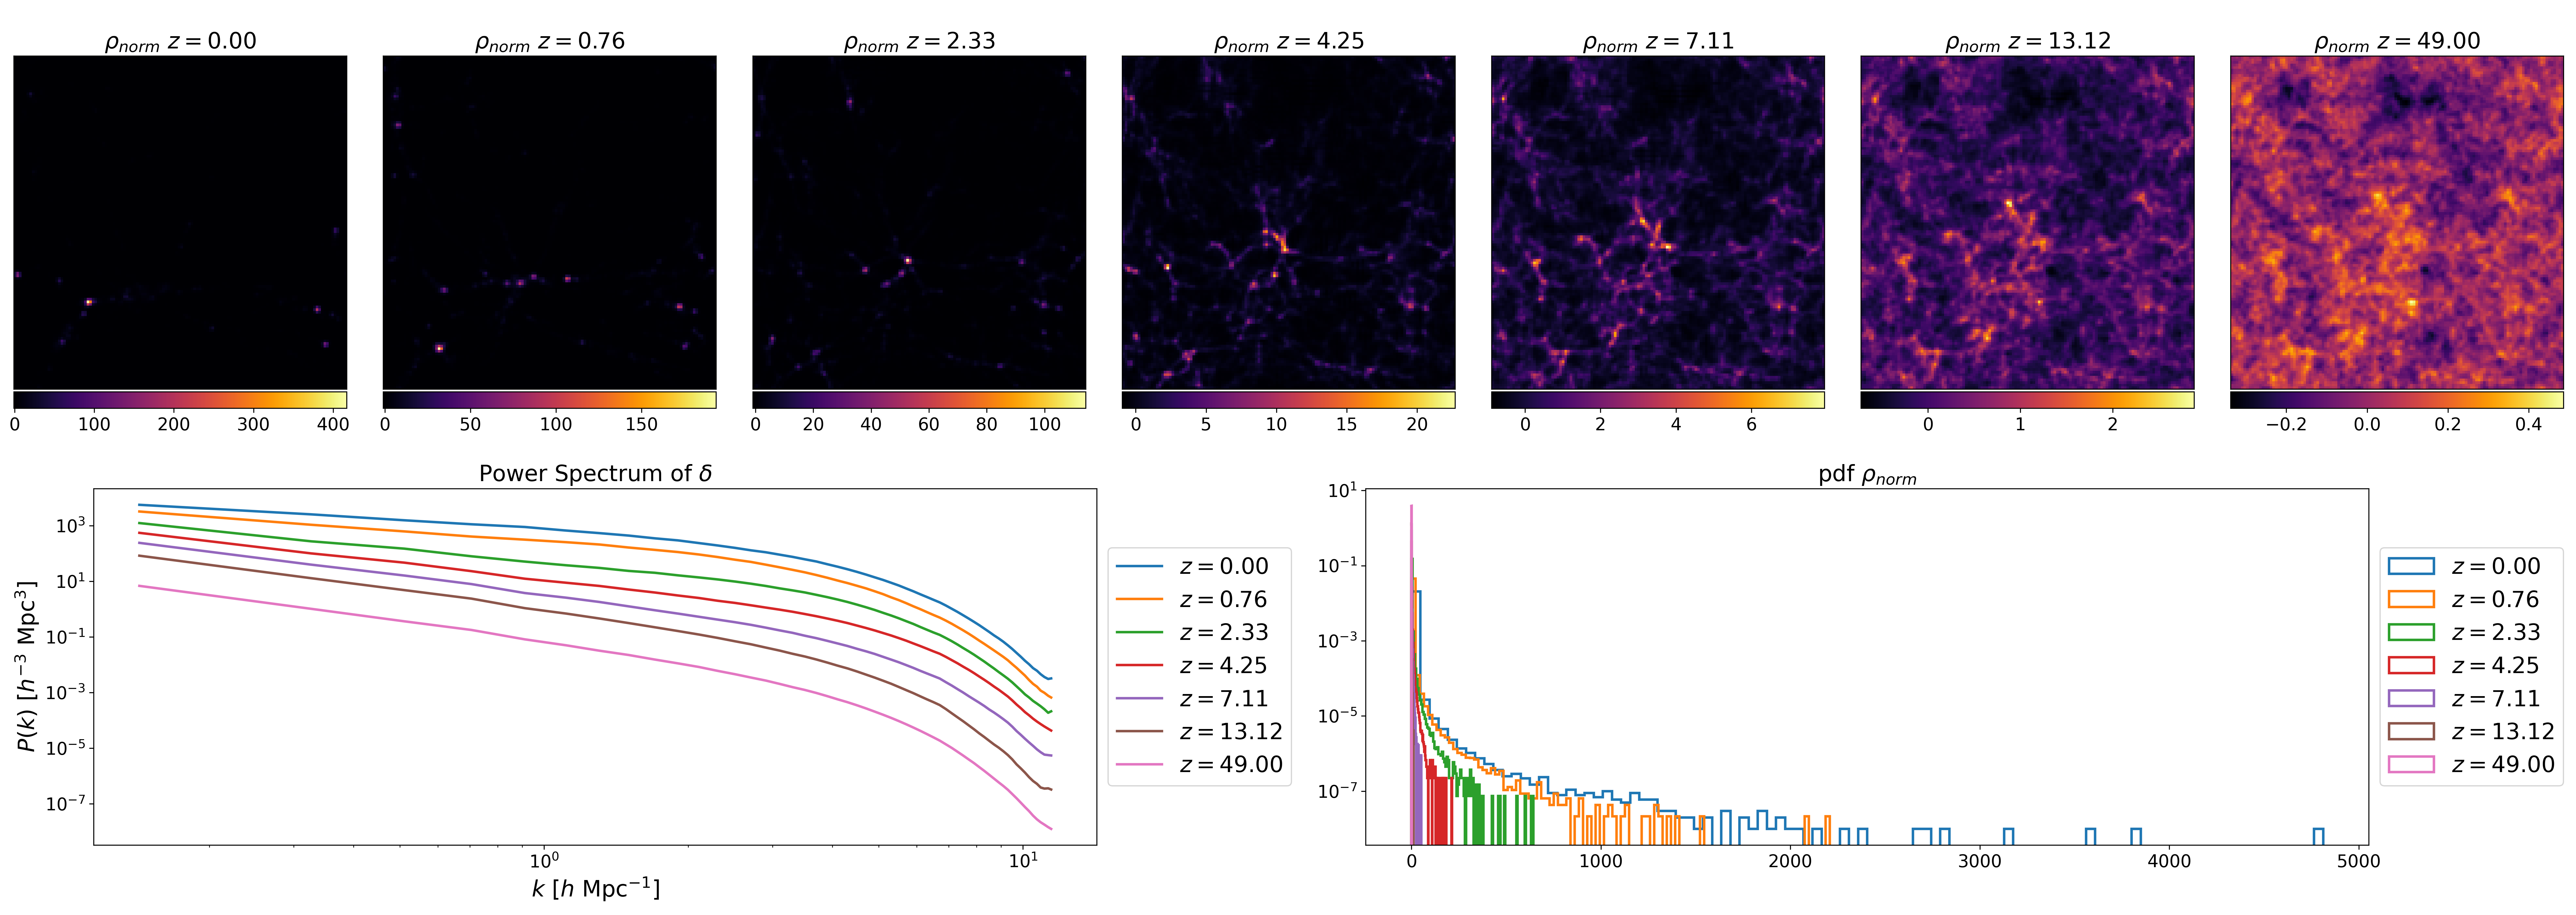
\includegraphics[width=1\linewidth]{img/delta.png}
    \caption{Distribution of overdensity at selected redshifts, illustrating complex structure with subtle and high-valued peaks}
    \label{fig:ditr_delta}
\end{figure}

\subsubsection{Standard Score Normalization}

Normalization is widely applied in almost all machine learning disciplines. A closely related discipline to our application, is models trained for image masking. Here the min-max normalization and the Z-Score normalization are frequently used and are associated with increased network performance improvements \citep{patro2015normalization}. However, the min-max normalization is problematic, as it scales each sample from the dataset differently, and we wish to learn a uniform scaling. A challenge attributed with non-uniform scaling, is that the network, unless it is explicitly informed about the min and max, has no idea how to scale the distribution exactly. Hence, we try the Z-score normalization defined as 

\begin{equation}
    \rho_{ssn}(\mathbf{x}) = \frac{\rho(\mathbf{x}) - \overline{\rho}}{\mathrm{Var}[\rho]}.
\end{equation}

Where its inverse can be derived as

\begin{equation}
    \rho(\mathbf{x}) = \rho_{ssn}(\mathbf{x}) \cdot \mathrm{Var}[\rho] + \overline{\rho}.
\end{equation}

A sample from the small dataset, with the Z-score normalization applied, can be seen in figure \ref{fig:z-score}. Unfortunately, the picture does not look a lot better, than with the overdensity normalization. Again, the cosmic web is not visible, and even though the CDF looks a bit better for density fields in the higher Redshift area, the values still tend to be squeezed into a small region around zero.

\begin{figure}[h]
    \centering
    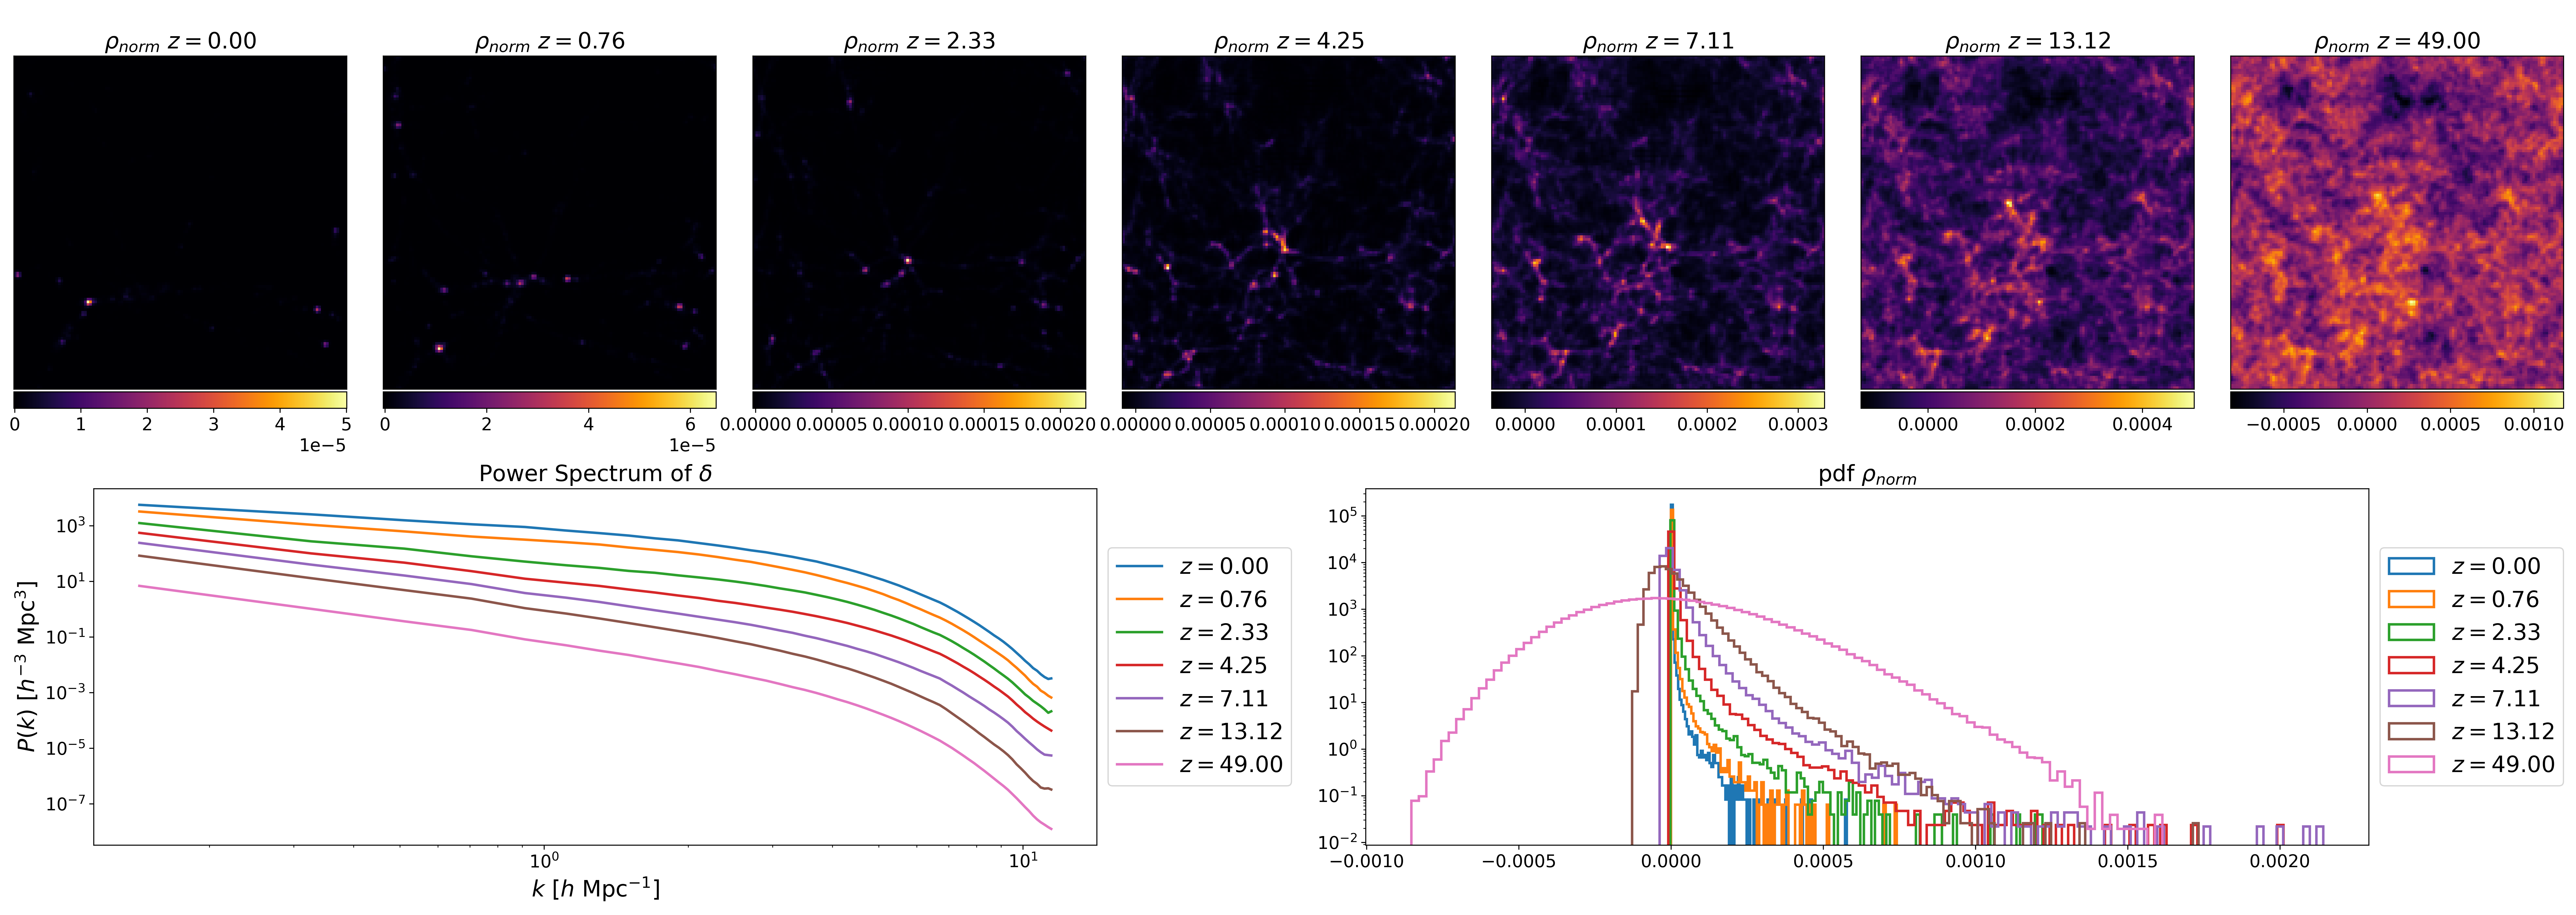
\includegraphics[width=1\linewidth]{img/ssm.png}
    \caption{Z-score normalization of the data distribution, facilitating a more uniform variance across the dataset}
    \label{fig:z-score}
\end{figure}

\subsubsection{Log Growth Normalization}

For our next normalization, we use a log scaling. The log scaling ensures the visibility of low density structures and reduces the impact of high density structures on the image and therefore the learning process. Furthermore, we include a scaling factor which is linearly dependent on the growth factor $D_+$. The initial time after the Redshift 49 is dominated by linear effects, which can essentially be approximated by

\begin{equation}
    \frac{\rho(\mathbf{x}, t_{l})}{D_+(t_l)} \approx \rho(\mathbf{x}, t_0).
\end{equation}

We simplify the approximated growth factor as defined in Equation \ref{eq:growth} by approximating it by $a$. The normalization is then expressed as

\begin{equation}
    \rho_{lgn}(\mathbf{x}) = \log_{10}\left(\frac{\frac{\rho(\mathbf{x})}{10^2} + 1.5}{a}\right)
\end{equation}

And its inverse

\begin{equation}
    \rho(\mathbf{x}) = \left(10^{\rho_{lgn}}\cdot a - 1.5\right) \cdot 10^2.
\end{equation}

\begin{figure}[h]
    \centering
    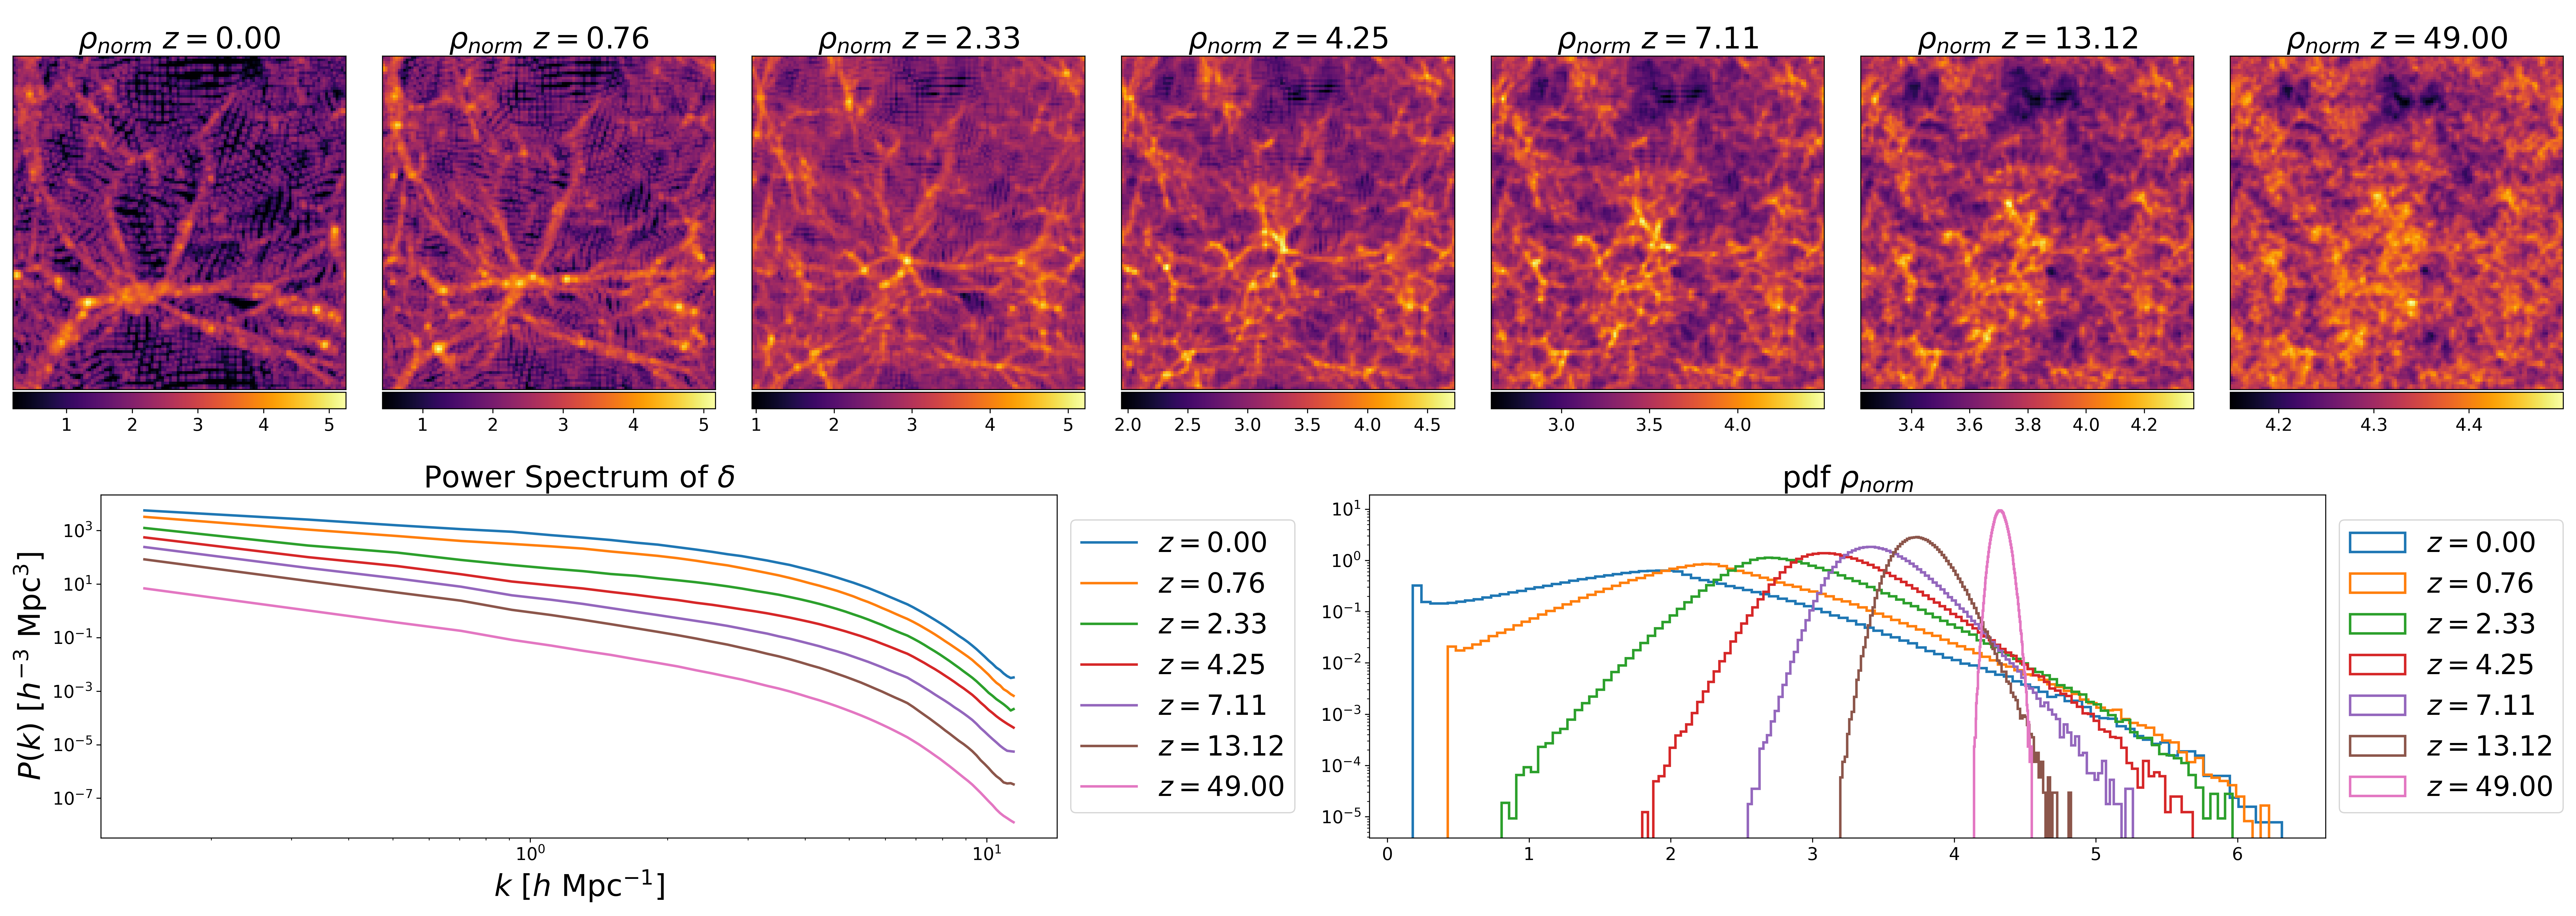
\includegraphics[width=1\linewidth]{img/log_growth.png}
    \caption{Log growth normalization, highlighting the linear regimen of early dynamic stages}
    \label{fig:log-growth}
\end{figure}

The log growth normalization can be observed in figure \ref{fig:log-growth}. Now finally we can observe the cosmic web and see a lot more structure is revealed. Furthermore, the CDF plot hints at a better distribution. Still, many values are cramped into the region around zero for low Redshift times, which is visible by the sharp jump of the CDF on the very left. However, this is not necessarily bad, as super low density regions are likely less important for the predictions.

\subsubsection{Normalization Conclusion}

When trying to learn a model on the dataset, on predicting from $z=0$ to $z=49$, the only normalization function which does result in an immediate overfitting pattern is the one which is trained on the Log Growth normalized dataset. Overfitting is the process, when the validation loss becomes increasingly higher, while the training loss decreases. This happens when the model starts memorizing the training data instead of learning to generalize to out of distribution data. To conclude, we identify the log growth normalization as the only working normalization method.

\subsection{Network Architecture}

We have considered denoising diffusion architectures, which have become the state of the art for conditional image generation \citep{denoising}. However, the requirement to have such a large dataset renders them unappealing in our case. In our case, the dataset cannot be pulled from the internet as it is the case for image generation algorithms, as each data point needs to be generated with a significant computational effort. Furthermore, we explored Conditional Adversial Generative Networks ({CGAN}) in section \ref{CGAN}; however, we think the training process is extremely challenging to get right, as the capabilities of the actor and critic need to be in a good balance. Since we have implemented a differentiable power spectrum, the critics from the CGAN framework can simply be replaced by mixing the defect of the generated power spectrum with the MSE. 
Finally, we have explored compressing the dataset into a lower dimensional latent space using decoder and encoder-based approaches. We could then perform the predictions in latent space, which could drastically reduce the size of the datasets during training. However, our experiments in section \ref{encoder-decoder} have indicated encoder decoder architectures do not work well for cosmological density data. 
Hence, we rely on the neural network architectures FNO and UNet as described in section \ref{nno}. The {UNet}, which is a very general network which performs surprisingly well for surrogate training \citep{koehler2024apebench}. Furthermore, we detailed the FNO, which is specifically designed as a surrogate neural network architecture. In this section, we introduce a slightly adapted version of the FNO architecture.

\subsubsection{UNet}

We tested a Periodic 3D UNet implementation, which is identical to a regular UNet, but the convolutional layers are adapted to work in 3D space. Furthermore, all convolutional layers utilize periodic boundary conditions, reflecting the ground truth we are training the network on. The UNet initially lifts the input channel, corresponding to a scalar matter density field, to 32 channels. The U-shaped architecture then consists of 2 layers. In our case, increasing the number of layers to more than two, resulted in an unstable learning pattern, where the UNet failed to converge to a solution. We now provide a fully reproducible description of the specific implementation of the UNet architecture. Recall the discrete convolutional operator

\begin{equation}
    (u \ast c)[\mathbf{v}, c] = \sum_{i \in \{0, \dots, c_{in}\}} \sum_{\mathbf{x} \in \Omega_{-k}^{k}} u\left[m(s \cdot \mathbf{v} - \mathbf{x}, n), i\right] \cdot c[\mathbf{x}, c]
\end{equation}

and its transpose operation

\begin{equation}
    (u \ast c)[\mathbf{v}, c] = \sum_{i \in \{0, \dots, c_{in}\}} \sum_{\mathbf{x} \in \Omega_{-k}^{k}} u\left[m(\lfloor \mathbf{v} / s \rfloor - \mathbf{x}, n), i\right] \cdot c[\mathbf{x}, c],
\end{equation}

where $k$ is the kernel expansion size, whereas $2k + 1$ is the kernel size. $u$ is the input field, which in our case is the density field, $c$ is the learned convolutional kernel, $s$ is the stride and $c_{in}$ is the number of input channels. Our UNET, given an input density field of $(1, 64, 64, 64)$, performs the following operations in the left arc of the U-shaped architecture in sequential order.

\begin{itemize}
    \item $(1, 64, 64, 64) \rightarrow (32, 64, 64, 64)$: Lift the channel number with a pixel wise fully connected neural network. That is a discrete convolutional operator with $s=1$, $k=0$ and $c_{in}=1$.
    
    \item $(32, 64, 64, 64)$: Store the projected tensor in the residuals list at index 0.
    
    \item $(32, 64, 64, 64) \rightarrow (32, 32, 32, 32)$: Downsample the tensor using a convolutional layer with a stride of two and a kernel size of three. That is a transpose discrete convolutional operator with $s=2$, $k=1$ and $c_{in} = 32$ followed by one with $s=1$, $k=1$ and $c_{in} = 32$.
    
    \item $(32, 32, 32, 32) \rightarrow (64, 32, 32, 32)$: Double the number of channels and apply a shape-preserving convolutional layer with stride zero. That is a discrete convolutional operator with $s=1$, $k=0$ and $c_{in} = 32$ followed by one with $s=1$, $k=1$ and $c_{in} = 64$.
    
    \item $(64, 32, 32, 32)$: Store the projected tensor in the residuals list at index 1.
    
    \item $(64, 32, 32, 32) \rightarrow (64, 16, 16, 16)$: Downsample the tensor using a convolutional layer with a stride of two and a kernel size of three. That is a discrete convolutional operator with $s=2$, $k=1$ and $c_{in} = 32$ followed by one with $s=1$, $k=1$ and $c_{in} = 32$.
    
    \item $(64, 16, 16, 16) \rightarrow (128, 16, 16, 16)$: Double the number of channels and apply a shape-preserving convolutional layer with stride zero. That is a discrete convolutional operator with $s=1$, $k=0$ and $c_{in} = 32$ followed by one with $s=1$, $k=1$ and $c_{in} = 64$.
\end{itemize}

On the right arc, the UNet then performs

\begin{itemize}
    \item $(128, 16, 16, 16) \rightarrow (64, 32, 32, 32)$: Upsample the tensor using a transpose convolutional layer with a stride of two and a kernel size of three. That is a transpose discrete convolutional operator with $s=2$, $k=1$ and $c_{in} = 128$ followed by one with $s=1$, $k=1$ and $c_{in} = 32$.
    \item $(64, 32, 32, 32) \times (64, 32, 32, 32) \rightarrow (128, 32, 32, 32)$: Concatenate tensor with residual at index 1.
    \item $(128, 32, 32, 32) \rightarrow (64, 32, 32, 32)$: Reduce the channel number with a pixel wise fully connected neural network. That is a discrete convolutional operator with $s=1$, $k=0$ and $c_{in}=128$.
    \item $(64, 32, 32, 32) \rightarrow (32, 64, 64, 64)$: Upsample the tensor using a transpose convolutional layer with a stride of two and a kernel size of three. That is a transpose discrete convolutional operator with $s=2$, $k=1$ and $c_{in} = 64$ followed by one with $s=1$, $k=1$ and $c_{in} = 32$.
    \item $(32, 64, 64, 64) \times (32, 64, 64, 64) \rightarrow (64, 64, 64, 64)$: Concatenate tensor with residual at index 0.
    \item $(64, 32, 32, 32) \rightarrow (32, 32, 32, 32)$: Reduce the channel number with a pixel wise fully connected neural network. That is a discrete convolutional operator with $s=1$, $k=0$ and $c_{in}=64$.
    \item $(32, 32, 32, 32) \rightarrow (16, 64, 64, 64)$: Upsample the tensor using a transpose convolutional layer with a stride of two and a kernel size of three. That is a transpose discrete convolutional operator with $s=2$, $k=1$ and $c_{in} = 32$ followed by one with $s=1$, $k=1$ and $c_{in} = 32$.
    \item $(16, 64, 64, 64) \rightarrow (1, 64, 64, 64)$: Reduce the channel number with a pixel wise fully connected neural network. That is a discrete convolutional operator with $s=1$, $k=0$ and $c_{in}=16$.
\end{itemize}


\subsubsection{FNO}

We test a Fourier Neural Operator (FNO) with 16 hidden channels and 4 layers, adapted for 3D operations. The convolution is applied to all 32 modes, which corresponds to all available modes when trained on a $64^3$ shaped dataset. In sequential order, the FNO performs the following operations:

\begin{outline}[enumerate]
    \1 $(1, 64, 64, 64) \rightarrow (16, 64, 64, 64)$: Lift the channel number. That is a discrete convolutional operator with $s=1$, $k=0$ and $c_{in}=1$.
    \1 Apply the first FNO Layer:
        \2 Apply shape-preserving convolution and store it as a bypass. That is a discrete convolutional operator with $s=1$, $k=1$ and $c_{in} = 16$.
        \2 Project the quantity into Fourier space using a discrete Fourier Transform.
        \2 Apply complex matrix multiplication in Fourier space with the learnable complex weight matrix.
        \2 Project back into real space using discrete Fourier transform.
        \2 Add bypass to the result and apply activation function.
    \1 Apply layers 2, 3, and 4 which are identical to the first one, but with unique parameters.
\end{outline}


\subsubsection{Adapted FNO}

We introduce an Adapted Fourier Neural Operator with 16 hidden channels and 4 layers. In this case, the spectral convolution is applied to an increasing number of modes, leading to a lower parameter count.

\begin{outline}[enumerate]
    \1 $(1, 64, 64, 64) \rightarrow (16, 64, 64, 64)$: Lift the channel number. That is a discrete convolutional operator with $s=1$, $k=0$ and $c_{in}=1$.
    \1 Apply $i$-th FNO Layer for $i \in {0, 1, 2, 3}$, or respectively more if more layers are set.
        \2 Apply shape-preserving convolution and store it as a bypass. That is a discrete convolutional operator with $s=1$, $k=1$ and $c_{in} = 16$.
        \2 Project the quantity into Fourier space.
        \2 Apply complex matrix multiplication to the first $2^{\min((i + 3), M)}$ modes in Fourier space. Here $M$ is a parameter which sets the maximum number of modes.
        \2 Project back into real space using discrete Fourier transform.
        \2 Add the bypass to the result and apply the activation function.
    
\end{outline}

With the adapted FNO, the network initially learns the large-scale dynamics using the previous mode restricted spectral convolutional layers and subsequently refines the smaller scales in relation to these large-scale dynamics in the later layers. Its architecture allocates more computing power towards large-scale dynamics. Thanks to the bypass functions, the FNO can also transmit small-scale information from the input to any layer of the network.

\subsubsection{Network Architecture Conclusion}

We bench marked the three options by training each network for 20 epochs with a learning rate of 0.002 on the small dataset. For comparison metric we leverage the Residual Squared Error (RSE) which corresponds to 

\begin{equation}
RSE = \frac{\sum_{\mathbf{x} \in \Omega} \bigl(\rho(\mathbf{x}) - \hat{\rho}(\mathbf{x}) \bigr)^2}{\sum_{\mathbf{x} \in \Omega} \bigl(\rho(\mathbf{x}) - \overline{\rho}(\mathbf{x}) \bigr)^2}.
\end{equation}

The error measure compares and scales the method's Mean squared prediction error against a model predicting a constant density field with the correct mean. 

We found, when predicting from $z=4.25$ to $z=49$, that the adapted FNO achieved an RSE of 0.2, the traditional FNO reached an RSE of 0.25, and the UNet only achieved an RSE of 0.7. Hence, moving forward, we will use the adapted FNO. The UNet does not perform well in this instance because its architecture relies on embedding the entire distribution into a subspace of different dimensionality, known as the embedding space or latent space. Given the relatively low number of samples, learning such an embedding with the provided sample count is likely insufficient. Conversely, the FNO model is better suited to perturb the input distribution slightly.

\subsection{Hyperparameters}


\begin{figure}[h]
    \centering
    \includegraphics[width=0.4\linewidth]{img/channels_compute.png}
    \caption{Validation loss against compute time for different channel numbers in FNOs. The corresponding parameter count is denoted in the label of the plot.}
    \label{fig:channels-B}
\end{figure}


% \begin{figure}[h]
% \centering
% \subfloat[Visual and Power Spectrum comparison of predicted density fields with FNOs of different channel numbers. The top row shows the residual between the predictions and the ground truth. Red areas highlight regions where the prediction deposits too much mass, while blue areas indicate the opposite.]{\label{fig:channels-A}
% \centering
% 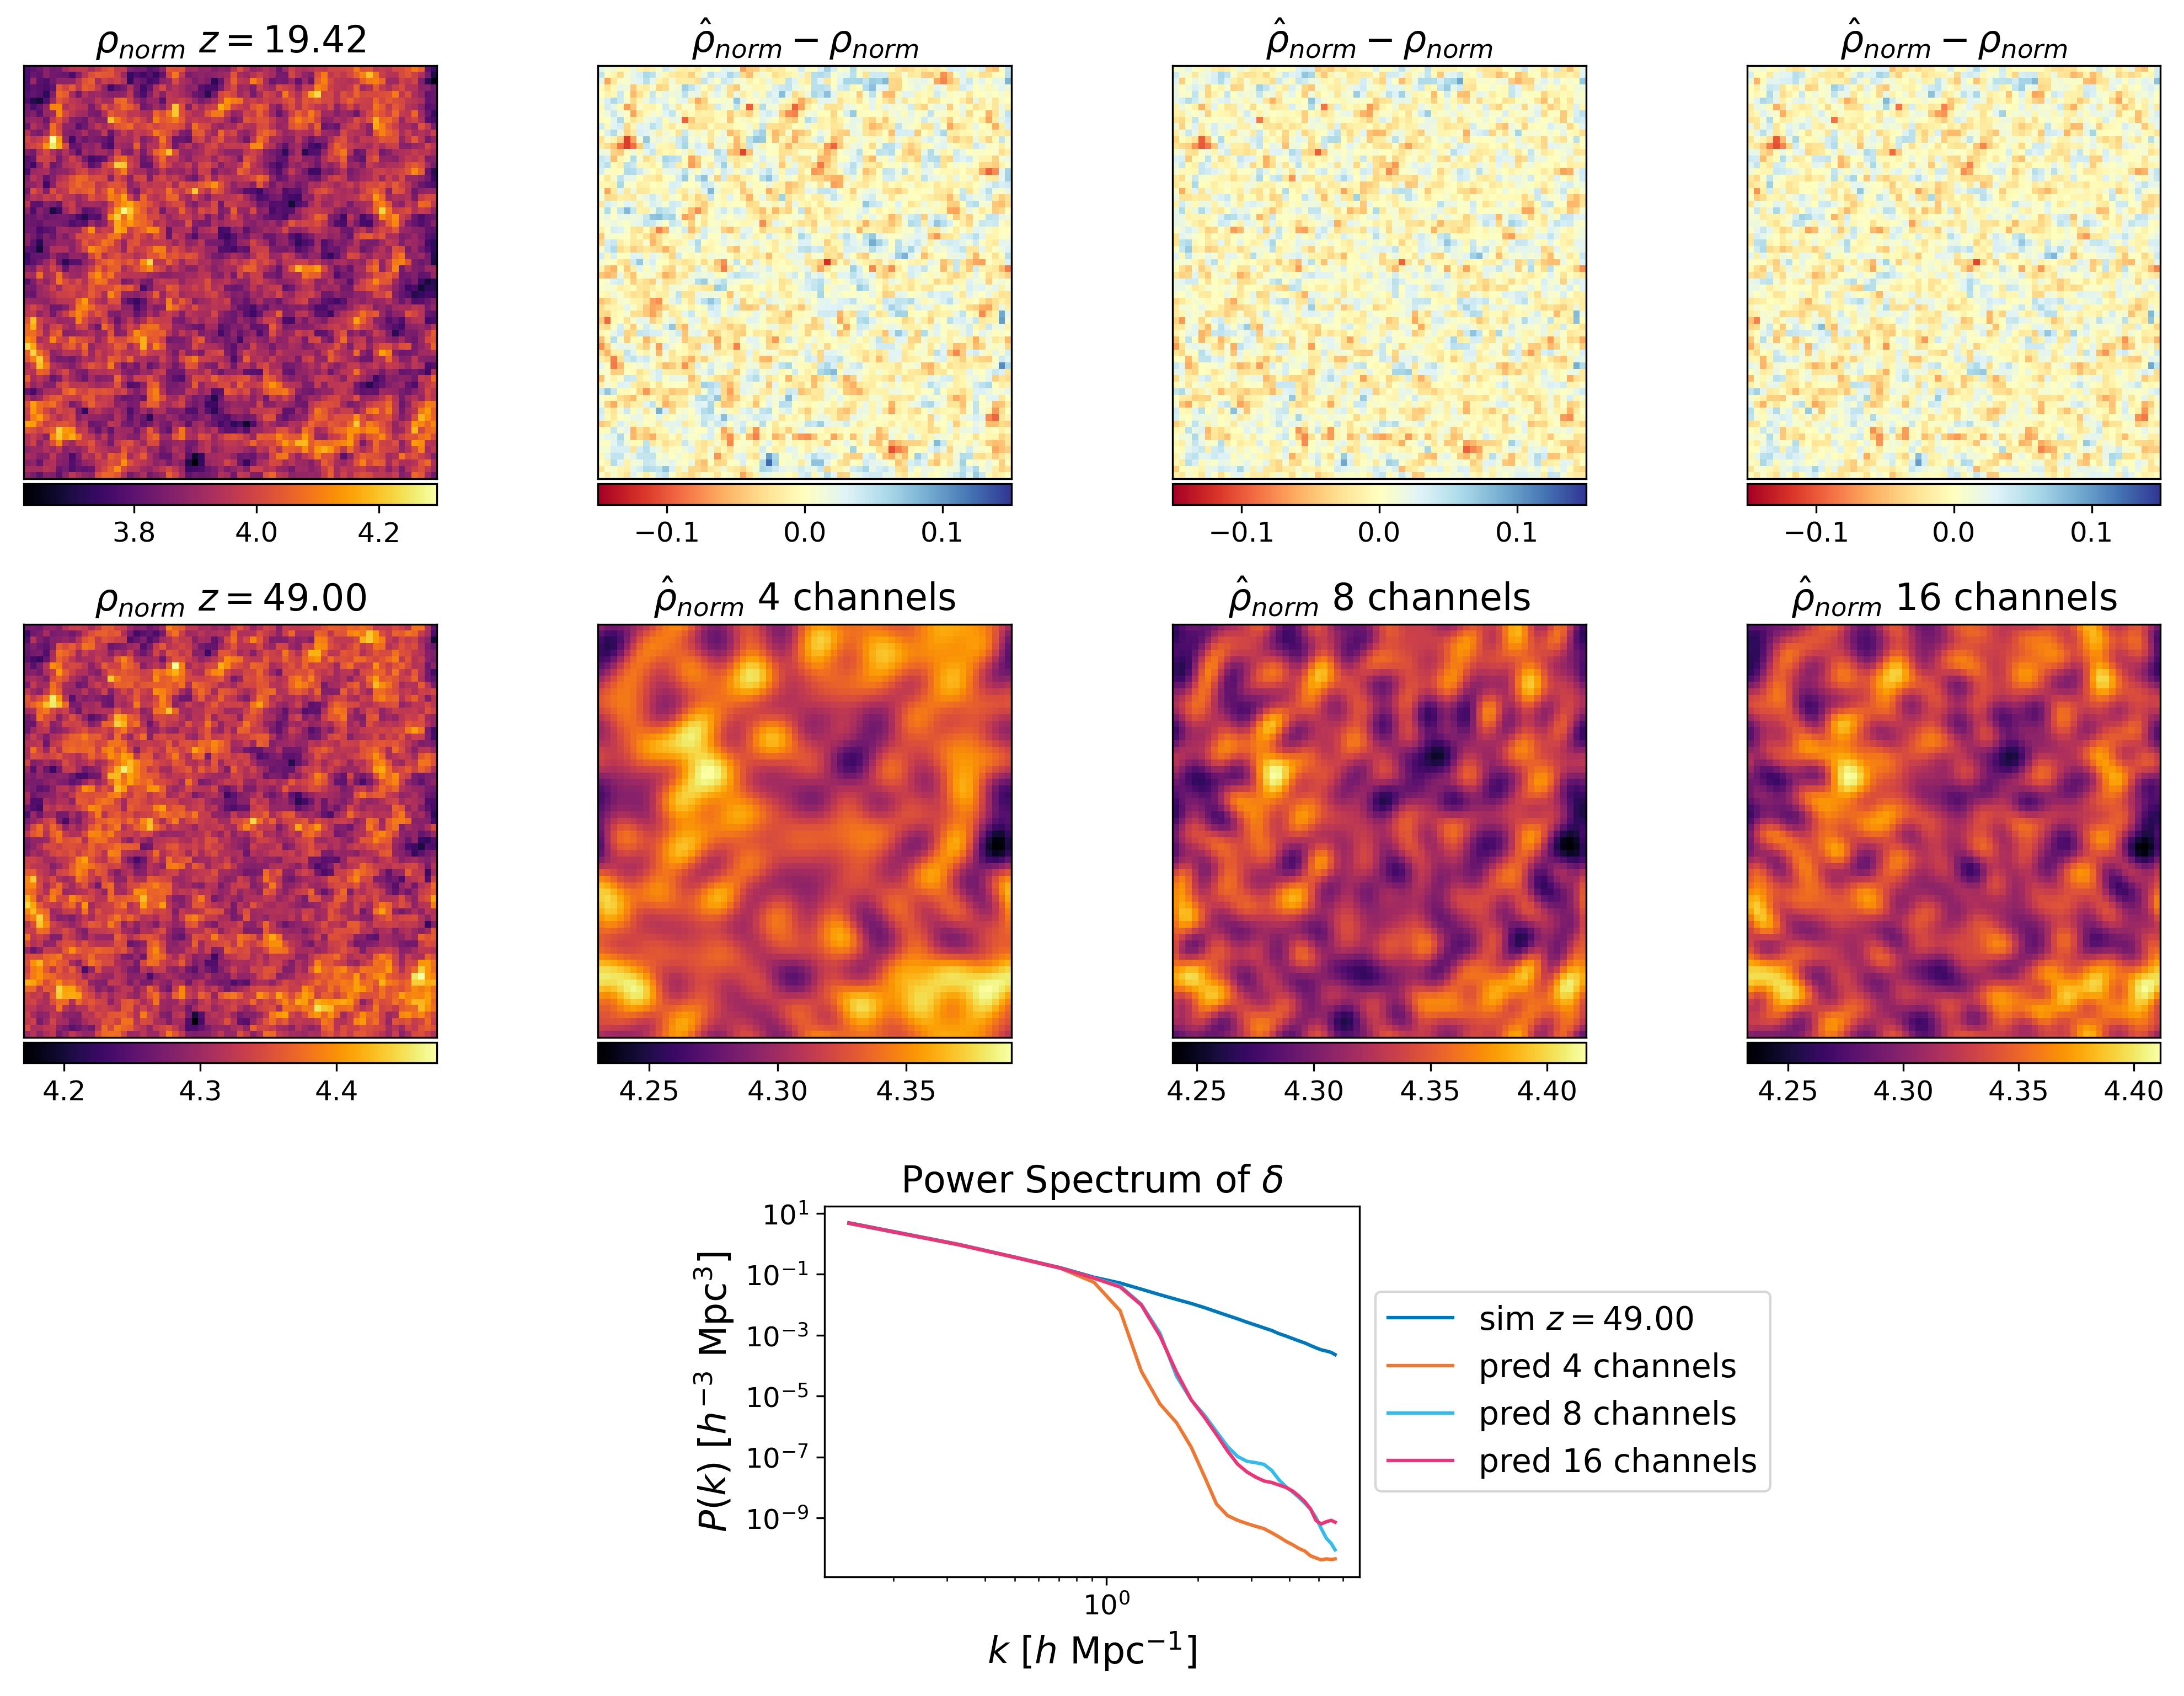
\includegraphics[width=0.6\linewidth]{img/compare_channels_3.jpg}
% }
% %no space
% \hfill
% \subfloat[Validation loss against compute time for different channel numbers in FNOs. The corresponding parameter count is denoted in the label of the plot.]{\label{fig:channels-B}
% \centering
% \includegraphics[width=0.35\linewidth]{channels_compute.png}
% }

% \caption{Comparison of predictions and validation convergence using different hidden channel numbers in FNO networks. Predictions are made from $z=4.25$ to $z=49$.}
% \label{fig:channels}
% \end{figure}


Instead of applying a gradient free hyperparameter optimization, we take a more nuanced approach, allowing us to balance network size with training efficiency. Training efficiency is often overlooked and becomes critical when training networks on datasets of this scale. The largest FNO we have tested has well over 30 million parameters. First we want to examine what the ideal number of channels is, that means how much should we lift the number of input channels in the first operation applied inside the FNO. To do so, we examine the predictions based on two observations. For one, we want to compare the actual predicted distribution visually and based on the power spectrum of predictions. But we are also interested in comparing the learning capacity of the model against its compute costs. Naturally, we favor a model which converges to the lowest validation loss after a certain time spent on training, whereas we assume time to be an equivalent measure to compute cost. When comparing models with different parameters, comparing the validation loss against the number of epochs can be misleading, as larger models usually require more computing time to finish a single epoch. We test train all models on 20 epochs with a learning rate of 0.002. In a first setup, we examine the effects on the training capacity of the model when using different numbers of channels, as seen in Figure \ref{fig:channels}. In subplot (b), we can observe how the networks with more channels take longer to complete the first epoch due to their significantly higher parameter count. However, even after completing the first epoch, the validation loss is lower compared to networks with fewer channels. Furthermore, the slope of the validation loss appears to correlate with the number of channels, meaning more channels result in a more negative slope. Finally, we observe more unstable training, evident in the wobbly validation loss curve. The more unstable training is likely rooted in the increased parameter count, which leads to a more complex loss surface topology. Since we rely on an identical learning rate, the trajectory of the optimizer passes multiple small hills and valleys, which then appear as a jagged line in the validation loss. After all, a gradient-based algorithm traces a specific path in the loss surface topology, whereas plotting the loss over the training time is equivalent to showing the height profile of the traced path. We conclude a hidden channel count of 16 is ideal, as the difference between the 8 channel setup already appears to show diminishing returns. In subplot (a) we can visually observe how the network with more hidden channels is capable of predicting a more detailed density field, which is also reflected in the power spectrum. There, the prediction made with 8 and 16 hidden layers has a power spectrum whose intensity falls off later than with 4 hidden channels.


\begin{figure}[t]
    \centering
    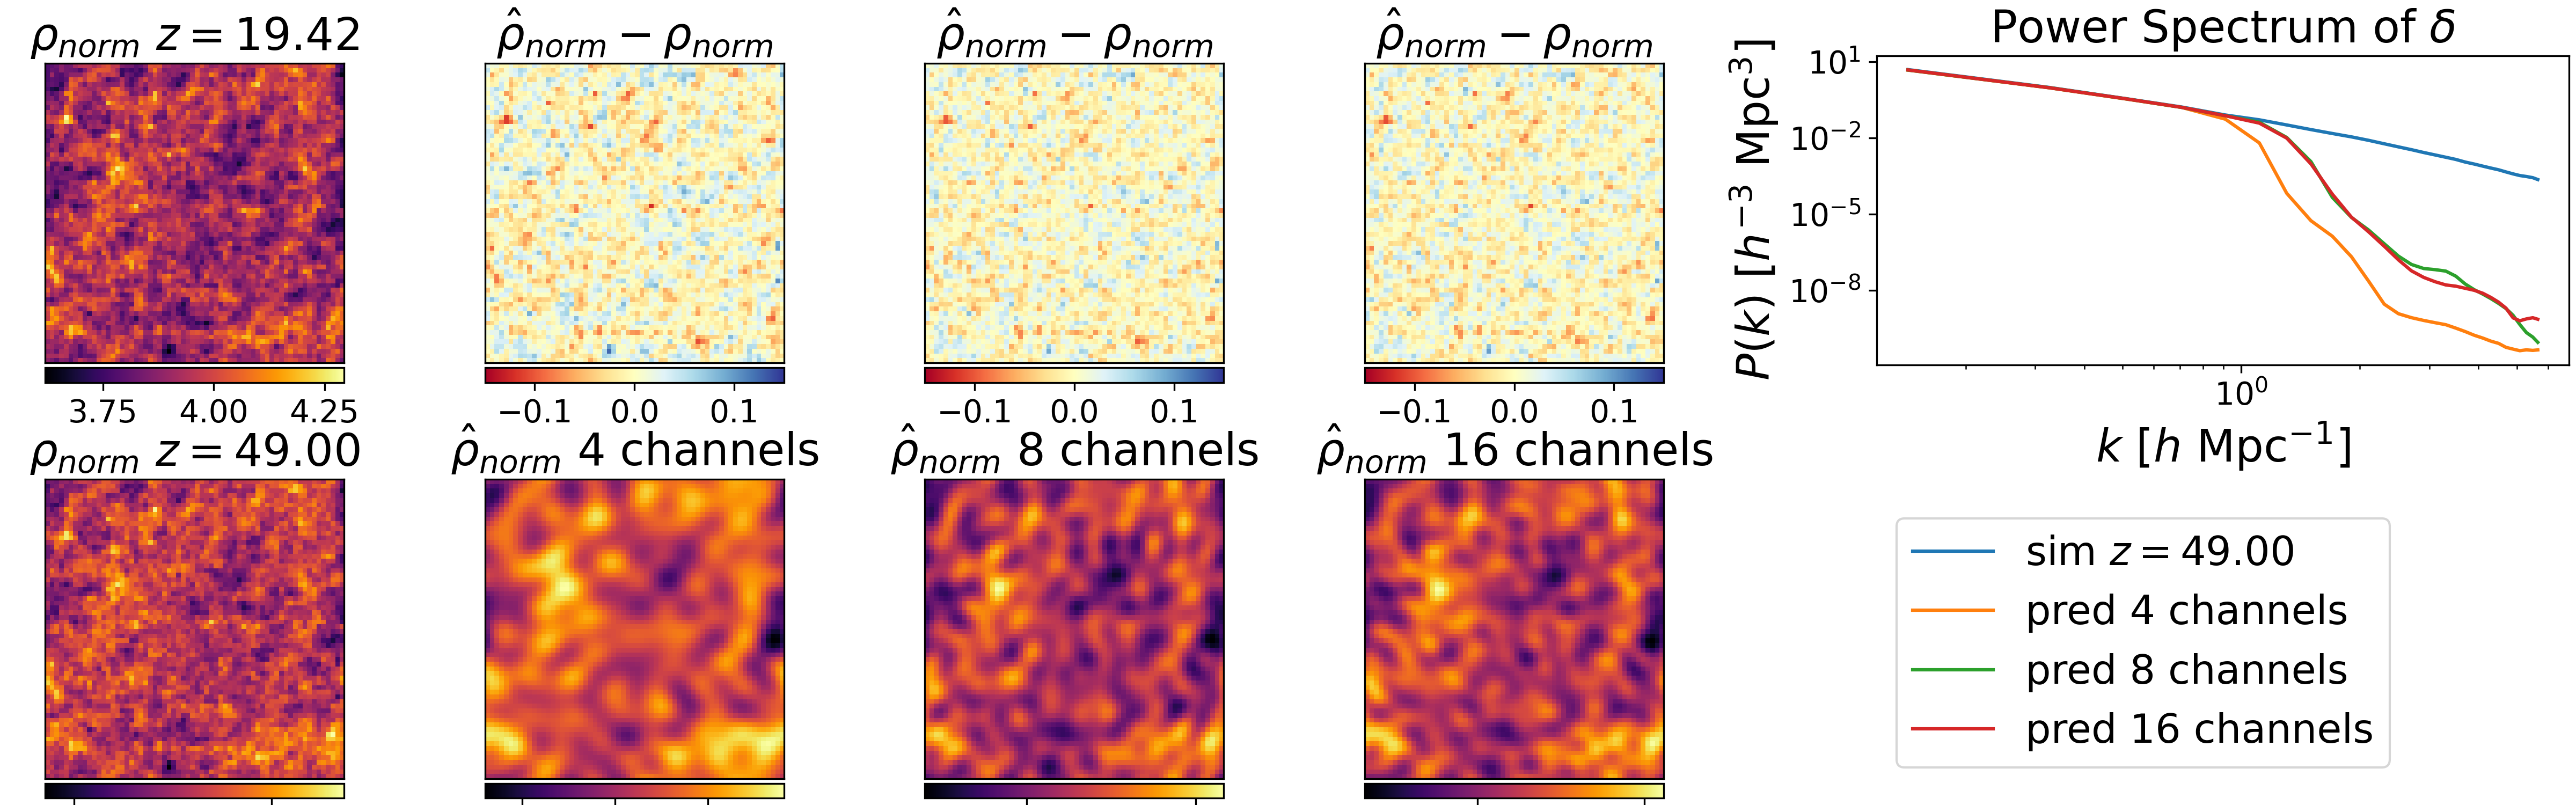
\includegraphics[width=0.95\linewidth]{img/compare_channels.png}
    \caption{Visual and Power Spectrum comparison of predicted density fields with FNOs of different channel numbers. The top row shows the residual between the predictions and the ground truth. Red areas highlight regions where the prediction deposits too much mass, while blue areas indicate the opposite.}
    \label{fig:channels-A}
\end{figure}


In a next step, we examine the effect of the layer count on the validation loss in figure \ref{fig:layers}. In subplot (b) we can observe how the validation loss decreases most with a four layer setup, whereas more or less layers result in worse models. The Same is reflected in the subplot (a) as we can observe models with 


\begin{figure}[h]
    \centering
    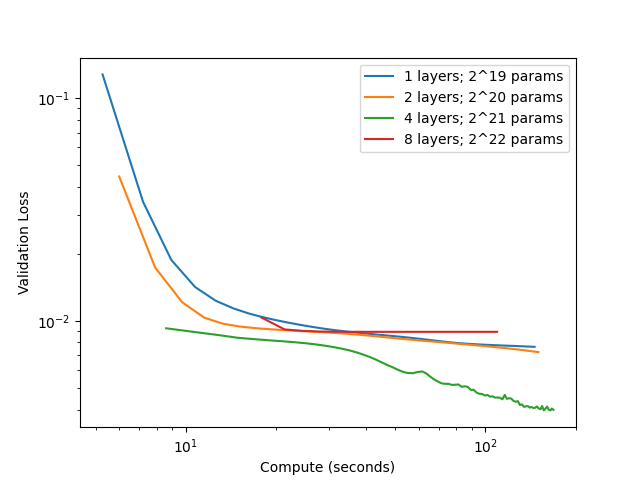
\includegraphics[width=0.4\linewidth]{img/layer_compute.png}
    \caption{Validation loss against compute time for different layer counts in FNO's. The corresponding parameter count is denoted in the legend of the plot.}
    \label{fig:layer-B}
\end{figure}

\begin{figure}[h]
    \centering
    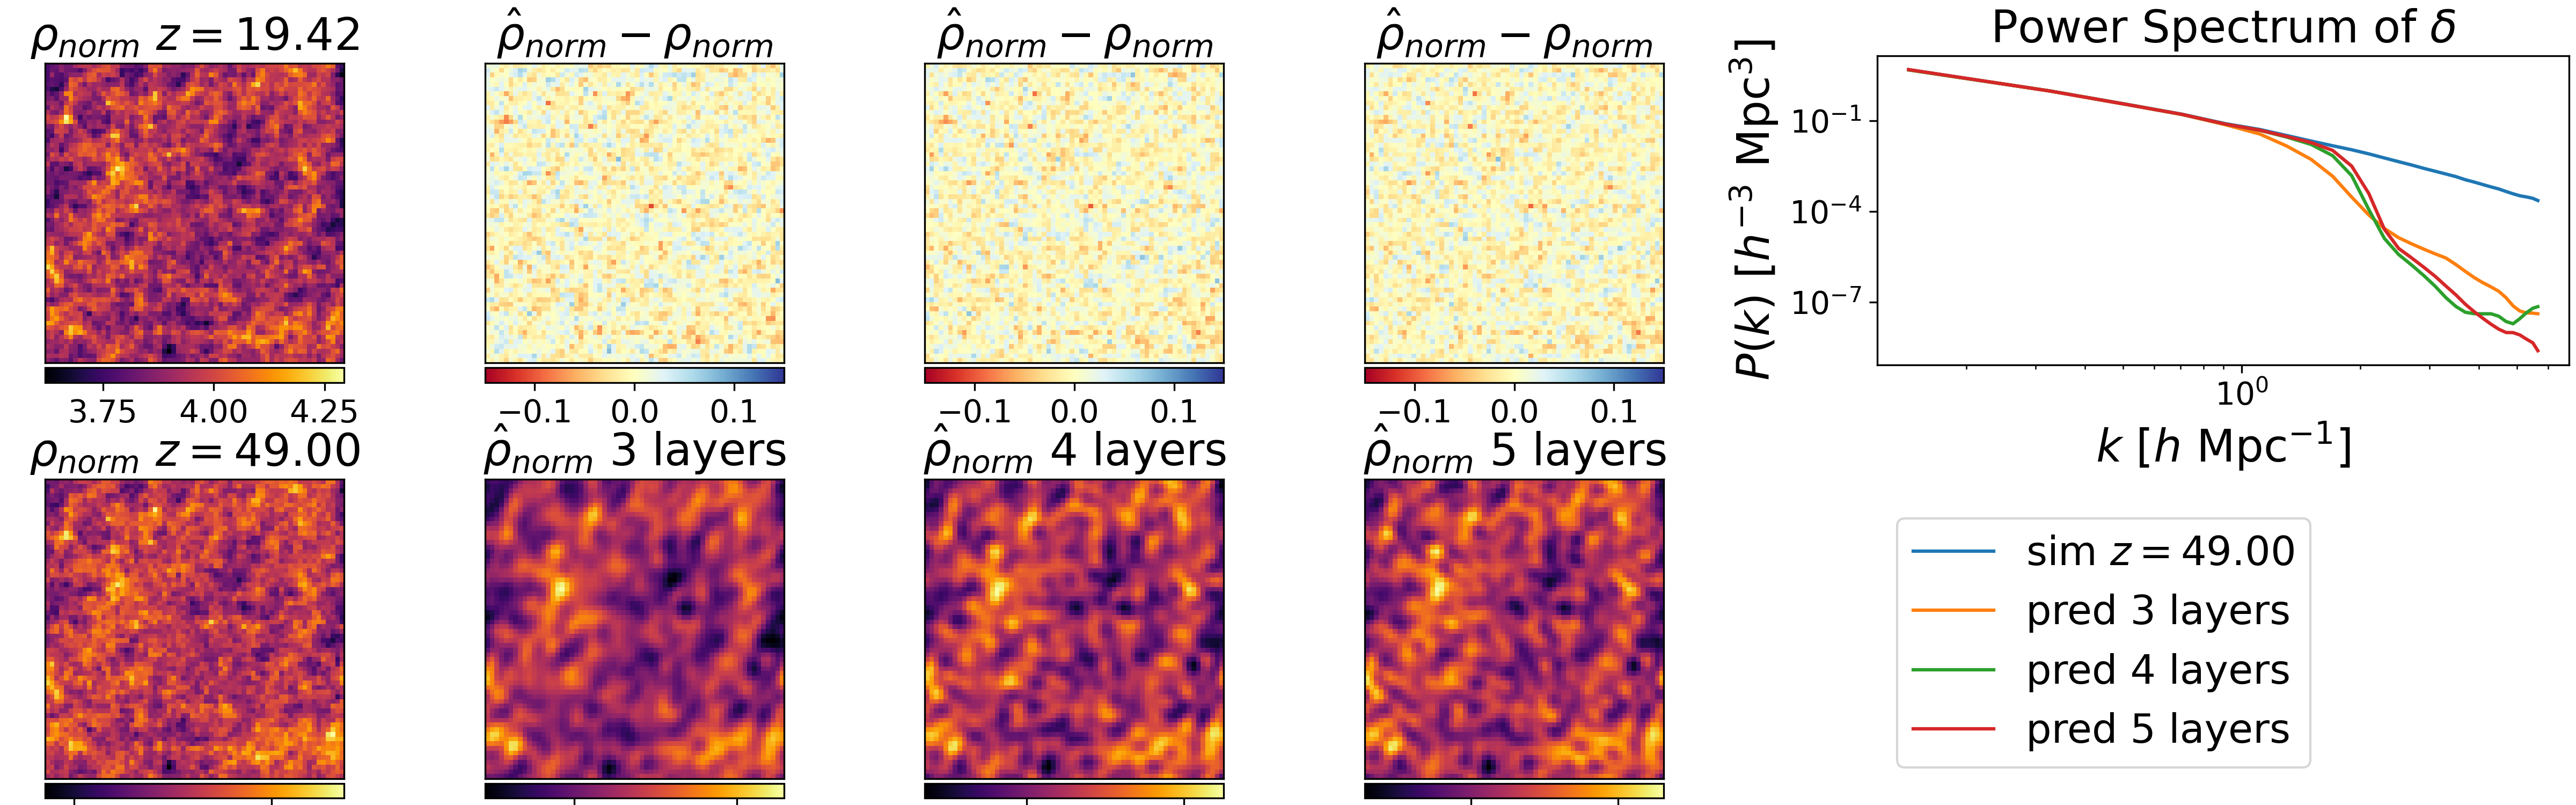
\includegraphics[width=0.95\linewidth]{img/compare_layers_2.png}
    \caption{Visual and Power Spectrum comparison of predicted density fields with FNO's of different different FNO layer counts. The top column shows the residual between the predicted and the ground truth. Red areas highlight areas where the prediction deposits too much mass, blue areas the opposite. }
    \label{fig:layer-A}
\end{figure}



\subsection{FNO Capabilities}

Interestingly, the FNO is capable of predicting a density and inherently follows the Power Spectrum accurately for lower k modes without explicitly extending the objective function with such a feature. Since the loss function is defined by a mean squared error, it might be argued that the power spectrum is actually captured by the mean squared error to some degree.
Our model is good at predicting the lower modes, which means it's effective at capturing large-scale dynamics with longer wavelengths. The difficulty in accurately predicting smaller structures can be attributed to the complex, nonlinear interactions governing the early universe. Furthermore, we complicate the prediction process, as the model has less information available about the distribution of the particles as a full N-Body solver during the forward prediction. Multiple particles with differing velocities can be jammed into a single grid cell, leading to a loss of information which is crucial for understanding the small-scale dynamics. This raises an interesting question: is the model just cutting off the higher modes and thus reshaping the output to fit expected patterns, or can it actually predict spatial changes caused by gravity? 

To better understand this, we compare the model's predictions against its inputs, where we artificially remove the the the shorter wavelengths. We achieve this by applying a discrete Fourier transform, setting entries in the complex matrix  associated with smaller scale structures to zero and then transforming the complex matrix back into a real space density field using the inverse Fourier transform. The results can be seen in figure \ref{fig:filter}. This method lets us compare the input and output distributions more easily. We set a wavelength cutoff such that the power spectrum of the filtered distribution starts to decrease at the same point as the predicted distribution. As expected, the power spectrum of these filtered distributions is different, since they come from a time with a lower redshift.

\begin{figure}[h]
    \centering
    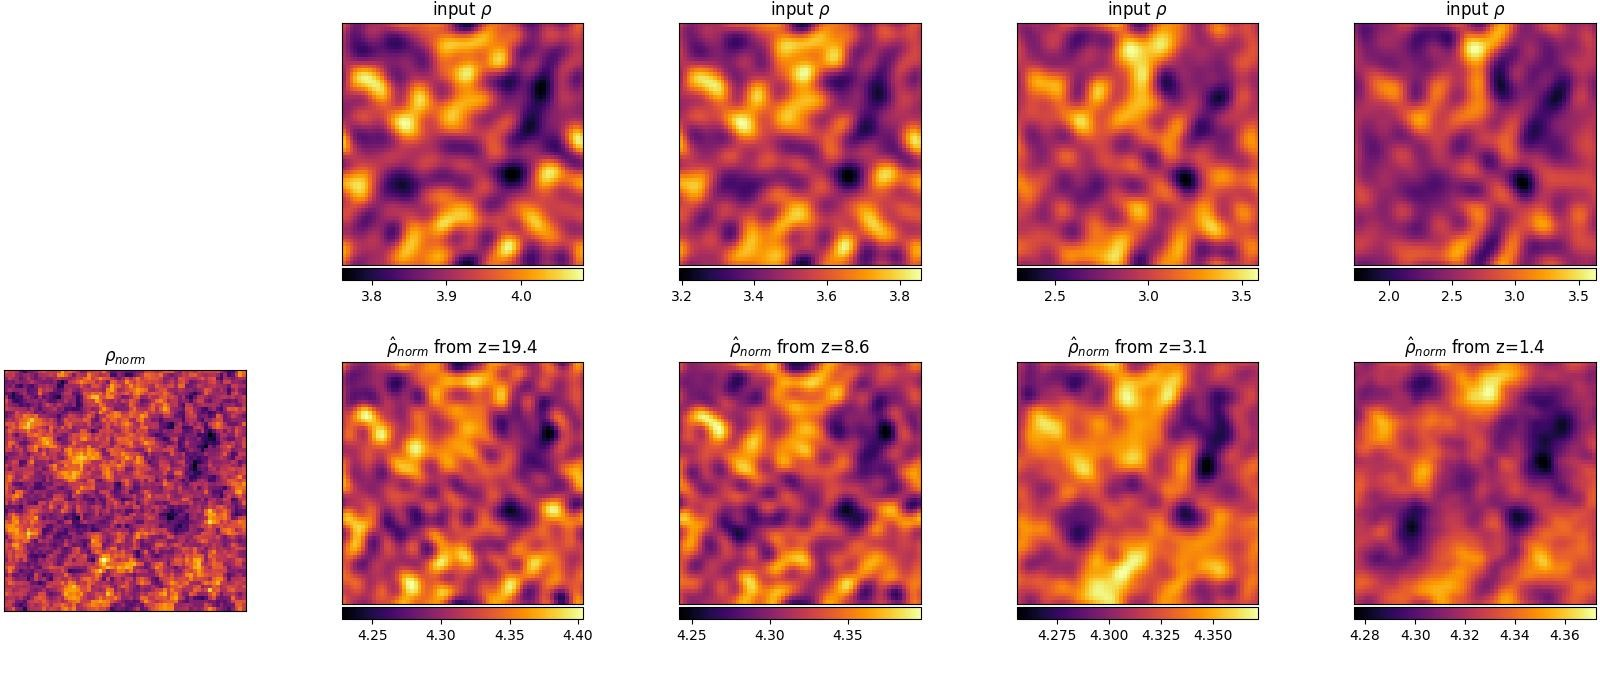
\includegraphics[width=0.9\linewidth]{img/compare_filtered.jpg}
    \caption{Top tow shows input distribution where k modes greater than 1 $h Mpc^{-1}$ are removed. The bottom row shows the prediction, where on very left is the ground truth of the simulation.}
    \label{fig:filter}
\end{figure}

When observing Figure \ref{fig:filter}, it becomes evident that the model is acquiring the ability to do more than simply blur the image by filtering out lower wavelengths. When comparing the top row with the bottom row, we can observe alterations to the underlying structure which have to be done with more complicated operations such as translations and diffusion's. This observation indicates how the network is not solely reliant on removing high-frequency components but is actively engaging in altering the distribution's characteristics. We have observed how our model struggles with small-scale strictures, and based on the visual results and the power spectrum, we assume it performs rather well on the large-scale structures. Let us test this hypothesis by removing all wavelengths smaller than $1MPC h^{-1}$ from the prediction and the simulation data. in figure \ref{fig:low-modes}, we can observe how larger modes are being predicted pretty accurately. On the very left, we can view the defect, where the error margin is around $10\%$.

\begin{figure}[h]
    \centering
    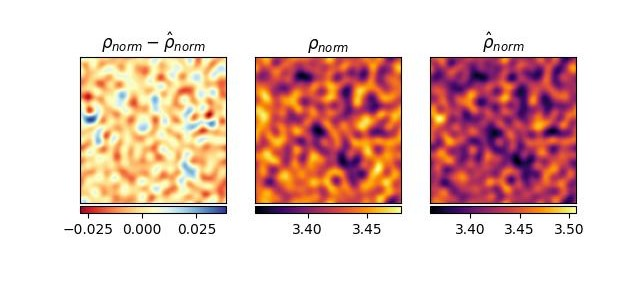
\includegraphics[width=0.5\linewidth]{img/distr_cmp.jpg}
    \caption{Prediction from $z=4.25$ to $z=49$ trained on the large dataset using a 5 layer adapted FNO and MSE.}
    \label{fig:low-modes}
\end{figure}


\subsubsection{Prediction Time Intervals}
\label{timeintervals}

Training the model on larger time spans is more difficult, which from a simulation perspective makes perfect sense. The longer the time span, the more computations are made in between; hence the network needs to predict a more complex operation. By alternating the initial Redshift of the distribution, which is used as the input for the network, we can observe a clear tendency. See figure \ref{fig:IC-comp}. The higher the Redshift of the input distribution, meaning the closer the time is to now, the less accurate the predictions become. More specifically, we can observe a correlation between the scale of the predicted structures and the size of the time interval. That is, the larger the time interval, the larger the threshold at which structures are not predicted anymore.
Visually, we can appreciate this as the predicted density fields appear more bury, as if a Gaussian blur or some sort was applied to them. 

\begin{figure}[h]
    \centering
    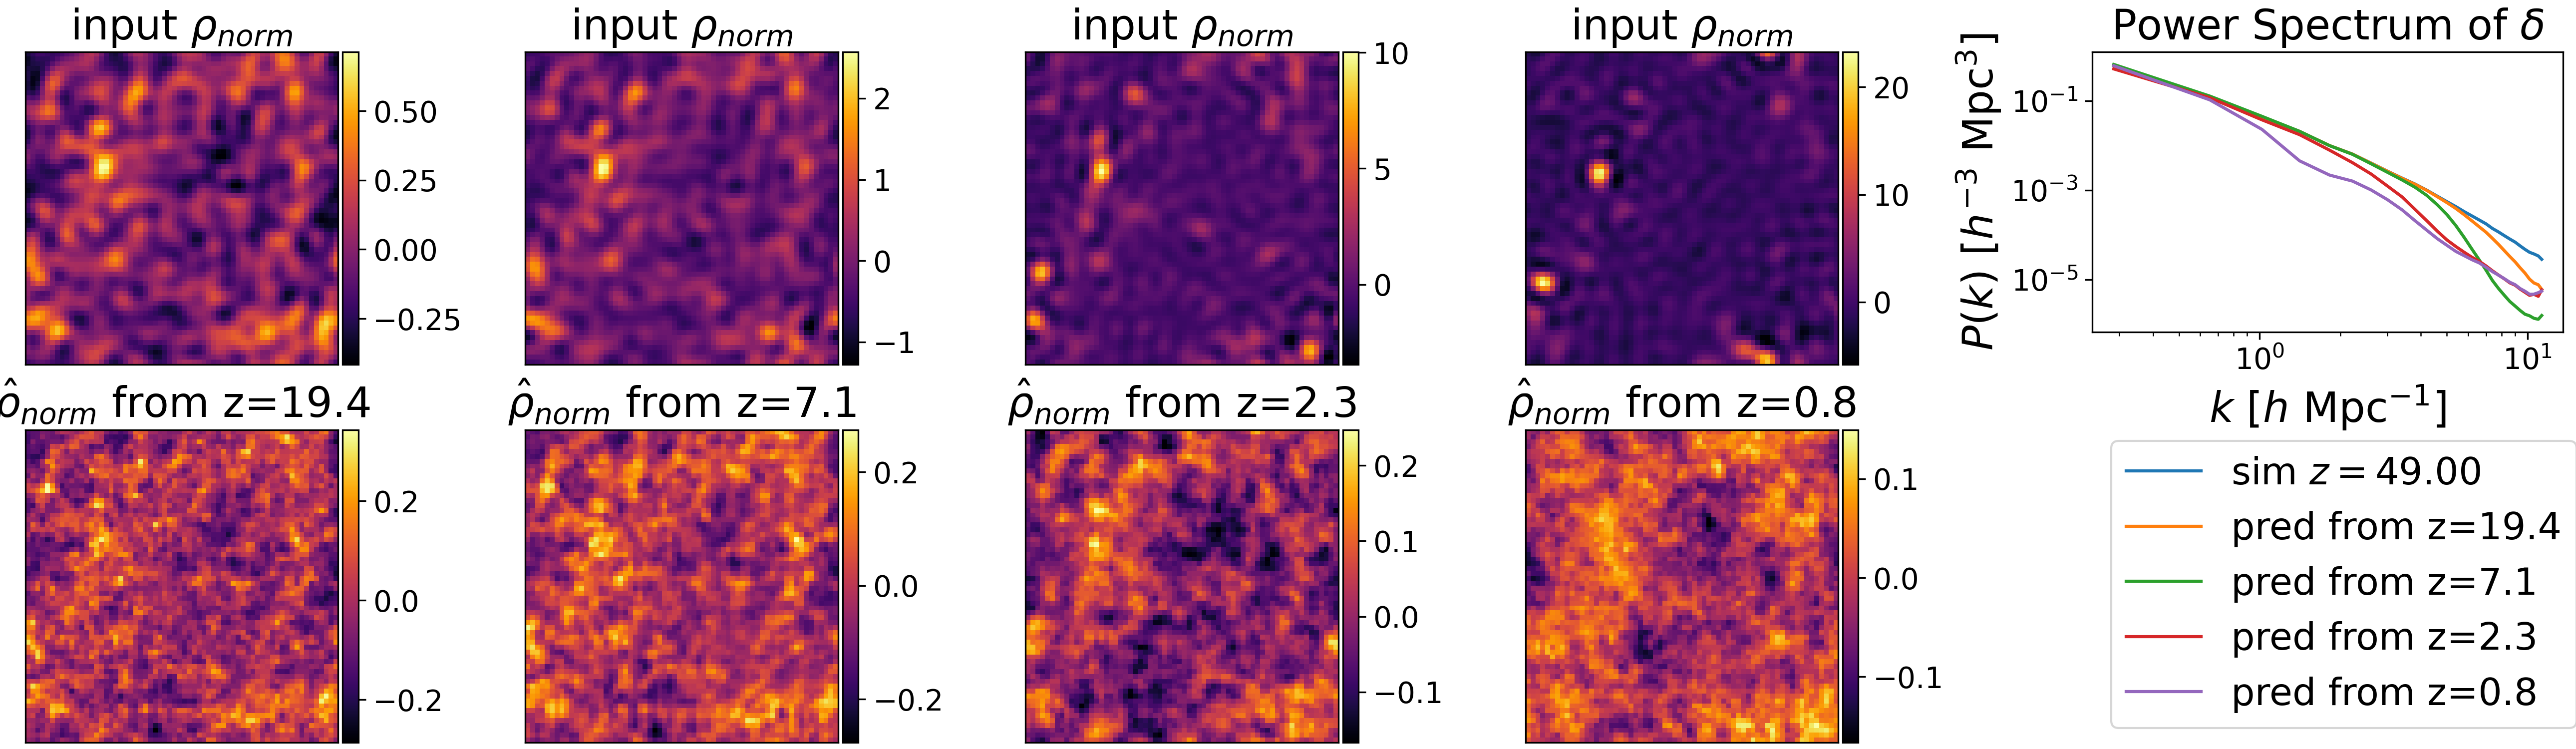
\includegraphics[width=0.9\linewidth]{img/compare_larger_scales.png}
    \caption{Comparison of identical FNO models trained on different time regions.}
    \label{fig:IC-comp}
\end{figure}

The same effect also affects the tendency to overfit a network, at least on the small dataset. The larger the time span, the earlier in the learning process the network is at risk of overfitting. Suggesting, the network is unable to learn actual dynamics, but resorts to simply memorizing the training dataset. To further verify this dynamics, we trained almost 30 unique models on specific time intervals. Each model starts at a different point in time and is trained on predicting for different time spans. The results can be seen in figure \ref{fig:ranges}, where expansion factor 1.0 denotes the current state of the universe, meaning at $z = 0$ and the expansion factor 0 is equivalent to $z=49$. In the topmost row, the previous hypothesis is confirmed once more. Notably, training neural networks on time ranges starting later in time, closer to now, is more successful.

\begin{figure}[h]
    \centering
    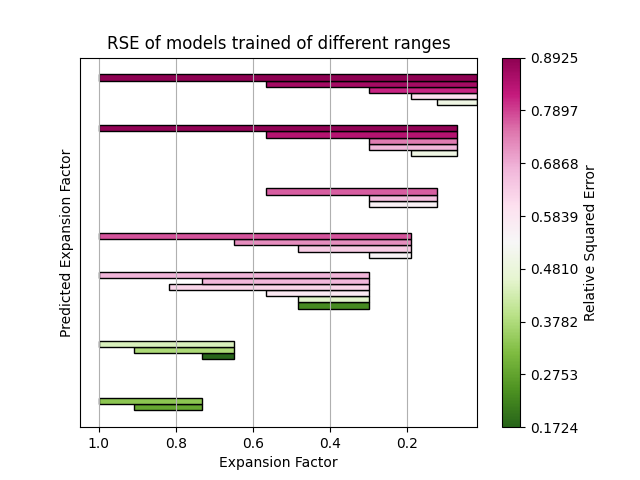
\includegraphics[width=0.7\linewidth]{img/ranges.png}
    \caption{Comparison of identical FNO models trained on different time regions.}
    \label{fig:ranges}
\end{figure}

\subsection{Further Enhancements}

In order to improve the performance of the neural network, we have investigated several approaches. In this section, we outline two of them, one being a different loss function and the other one additional feature engineering.

\subsubsection{Power Spectrum Loss}
\label{ps-loss}

\begin{figure}[h]
    \centering
    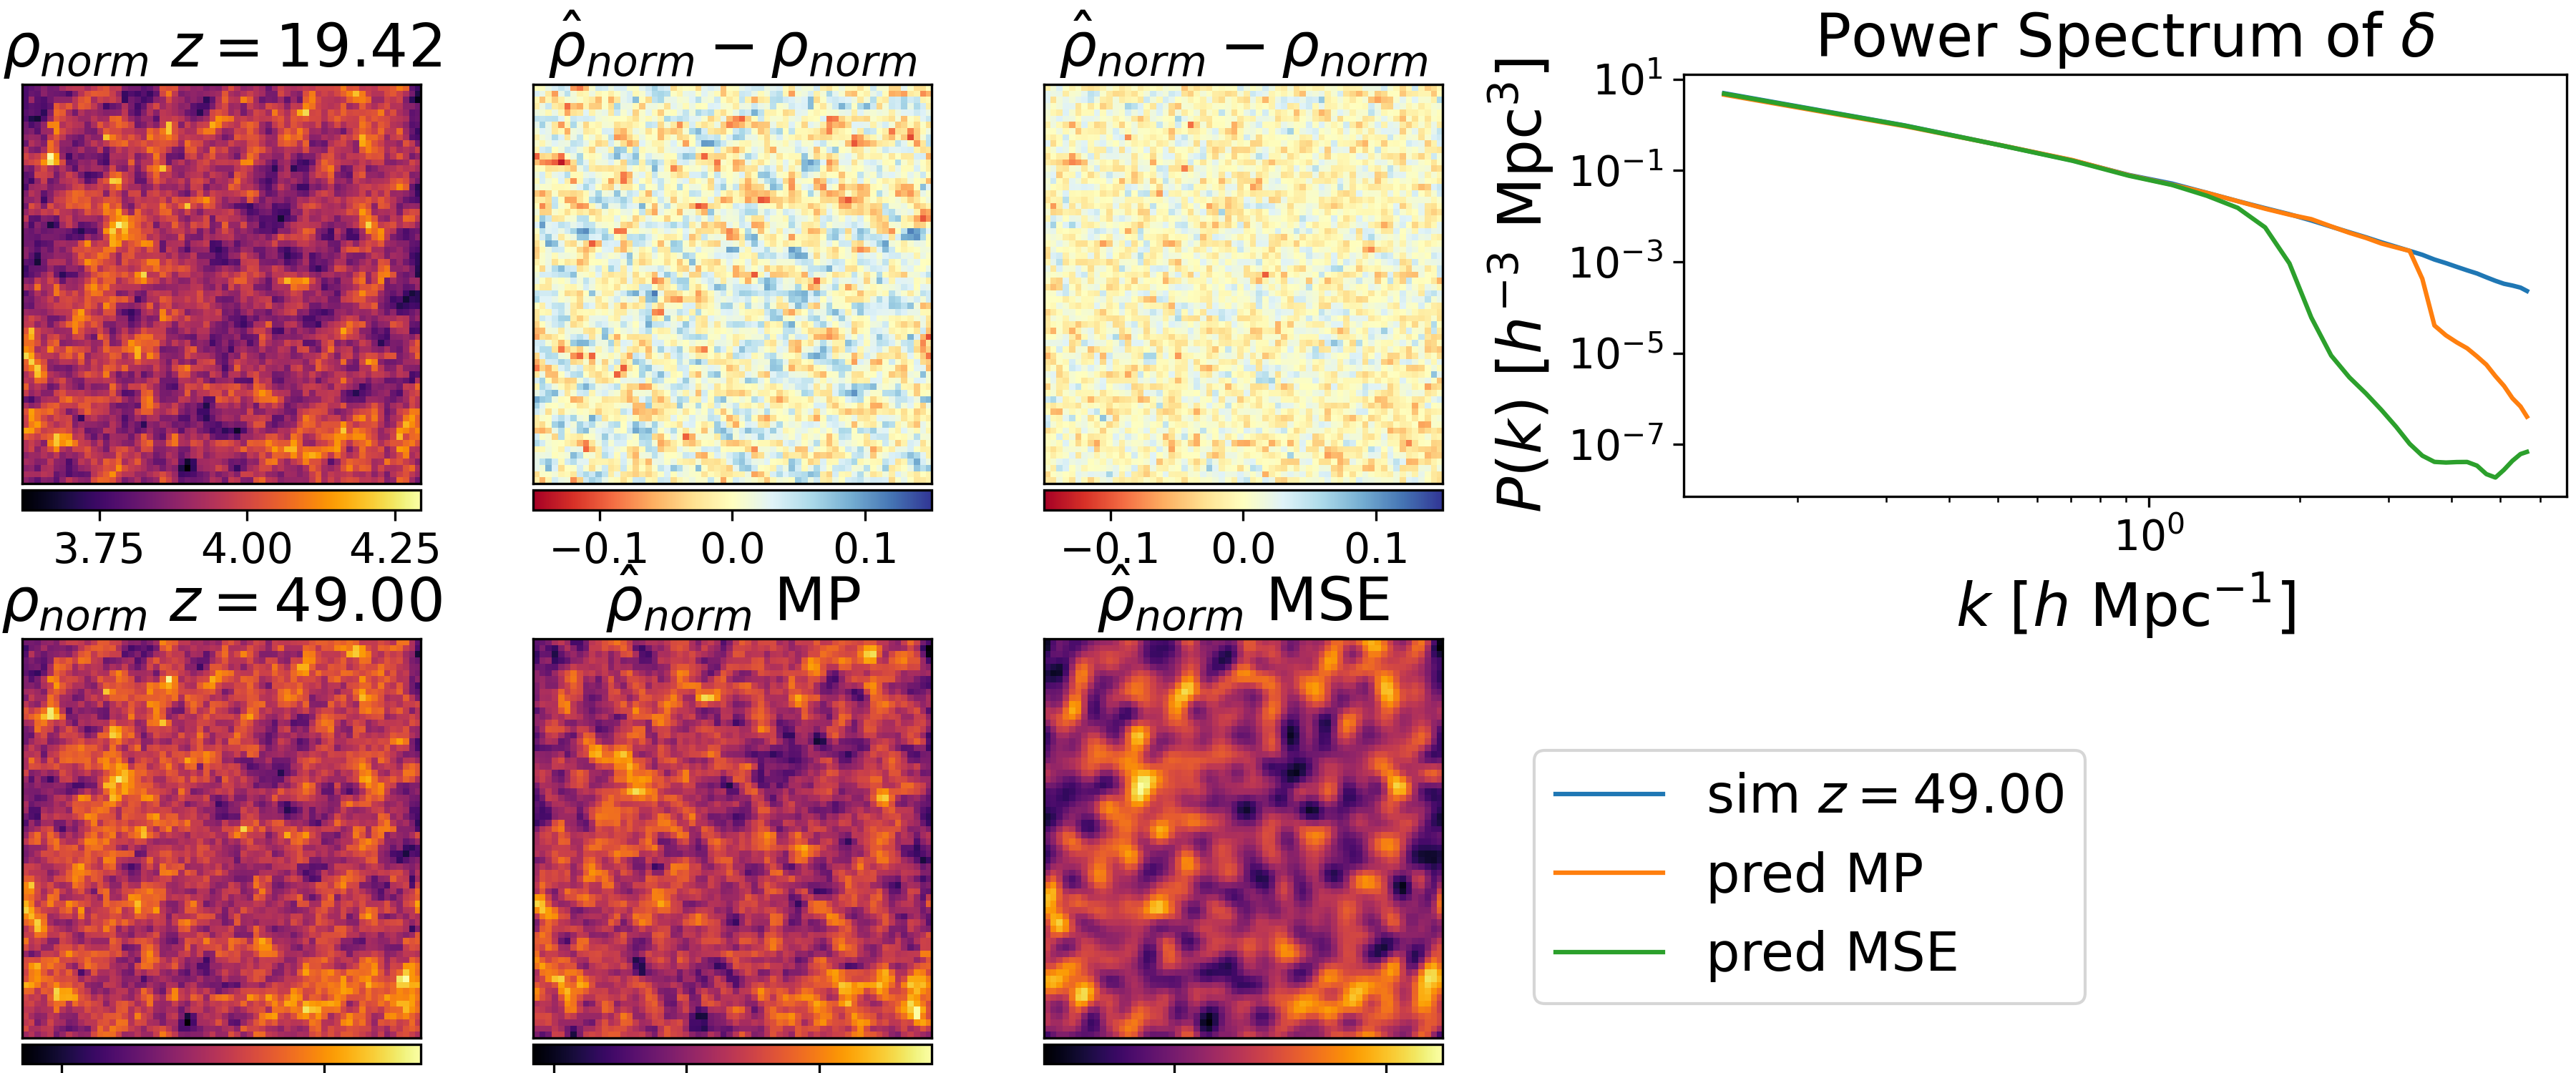
\includegraphics[width=0.8\linewidth]{img/compare_loss.png}
    \caption{Prediction from $z=19.2$ to $z=49$, compared with or without additional power loss term.}
    \label{fig:power-loss}
\end{figure}

As observed before, the network struggles to learn small scare structures. To increase the incentives to learn those structures, we include a power loss term into the object function. This means adding a mean squared measure of logarithmic deviation of the predicted density field power spectrum against the ground truth power spectrum. We intentionally use the logarithm to scale the values to a range comparable to the mean squared error of the normalized density field.
To force the network to learn the smaller scale structures, we adapt the loss term and define the power loss as

\begin{equation}
    L_{power} = \sum_{\mathbf{k} \in \Omega} \Biggl(  \log_{10} \Bigl( \langle |\delta(\mathbf{k}, t_0)|^2 \rangle \Bigr) - \log_{10} \Bigl( \langle |\delta(\mathbf{f}(\rho(\mathbf{x}, t_n))(\mathbf{k})|^2 \rangle \Bigr) \Biggr)^2.
\end{equation}

We then combine the power loss with the original MSE

\begin{equation}
    L_{MSE} = \sum_{\mathbf{x} \in  \Omega} \Biggl(\mathbf{f}(\rho(\mathbf{x}, t_{n})) - \rho(\mathbf{x}, t_0)\Biggr)^2,
\end{equation}

and obtain the MP loss function

\begin{equation}
    L_{MP} = \alpha \cdot L_{MSE} + \cdot L_{power}.
\end{equation}

The above requires a differentiable method of obtaining the power spectrum, which is not entirely straightforward. We will explain the details of the code in section \ref{impl}. When training a network with this function, the choice of $\alpha$ controls how much we value accuracy in terms of finding the same distribution versus obtaining a correct power spectrum. In Figure \ref{fig:power-loss}, we have plotted results from two networks: one trained using only $L_{MSE}$ and another using $L_{MP}$. The model trained with the Power Loss generally performs worse than the pure MSE model. Furthermore, the training process is very sensitive to the parameter $\alpha$; a poor choice can quickly lead to unfavorable outcomes. In our case, we found a value of $\alpha=2$,  slightly favoring the accuracy of density, to be working well. The training with the $L_{MSE}$ loss function achieved a Relative Squared Error (RSE) of 0.54, whereas the combined MSE and Power Spectrum loss yielded an RSE of 0.85 after 20 training epochs. In other words, the prediction with the power spectrum loss performed worse. However, we can also notice how the power spectrum of the prediction incorporating the power loss is significantly more accurate. This is also reflected in the visual comparison of the two density field predictions in figure \ref{fig:power-loss}. Here we can observe an increased presence of small structures. These small-scale features have many differing features from the ground truth, reflecting the decreased RSE accuracy score. For example, in the center region of prediction a few diagonal rays can be seen, those are not seen in the ground truth. Furthermore we can plot the Power Spectrum Correlation 


\begin{equation}
    P(\mathbf{k}) = \langle |\delta(\mathbf{k})| \cdot |\delta(\mathbf{k})_{pred}| \rangle,
\end{equation}

which gives us a measure of how well the predicted power spectrum correlates with the ground truth as seen in \ref{fig:power-loss-corr}. Interestingly when traied on the mean square error, the network does not appear to predict any fantasy structures, as the power spectrum falls of at an identical wavelength as the correlation function. This also means a mean squared error is good choice. We can conclude, that prediction that are made using a network trained on the mixed MP loss function perform a hybrid function of accurate density field predictions and generating fantasy small-scale structures to fit the desired power spectrum. The experiment highlights the generative capabilities of the FNO, to do such a task it has to be capable of learning to imprint a power spectrum into a density field.


\begin{figure}[h]
    \centering
    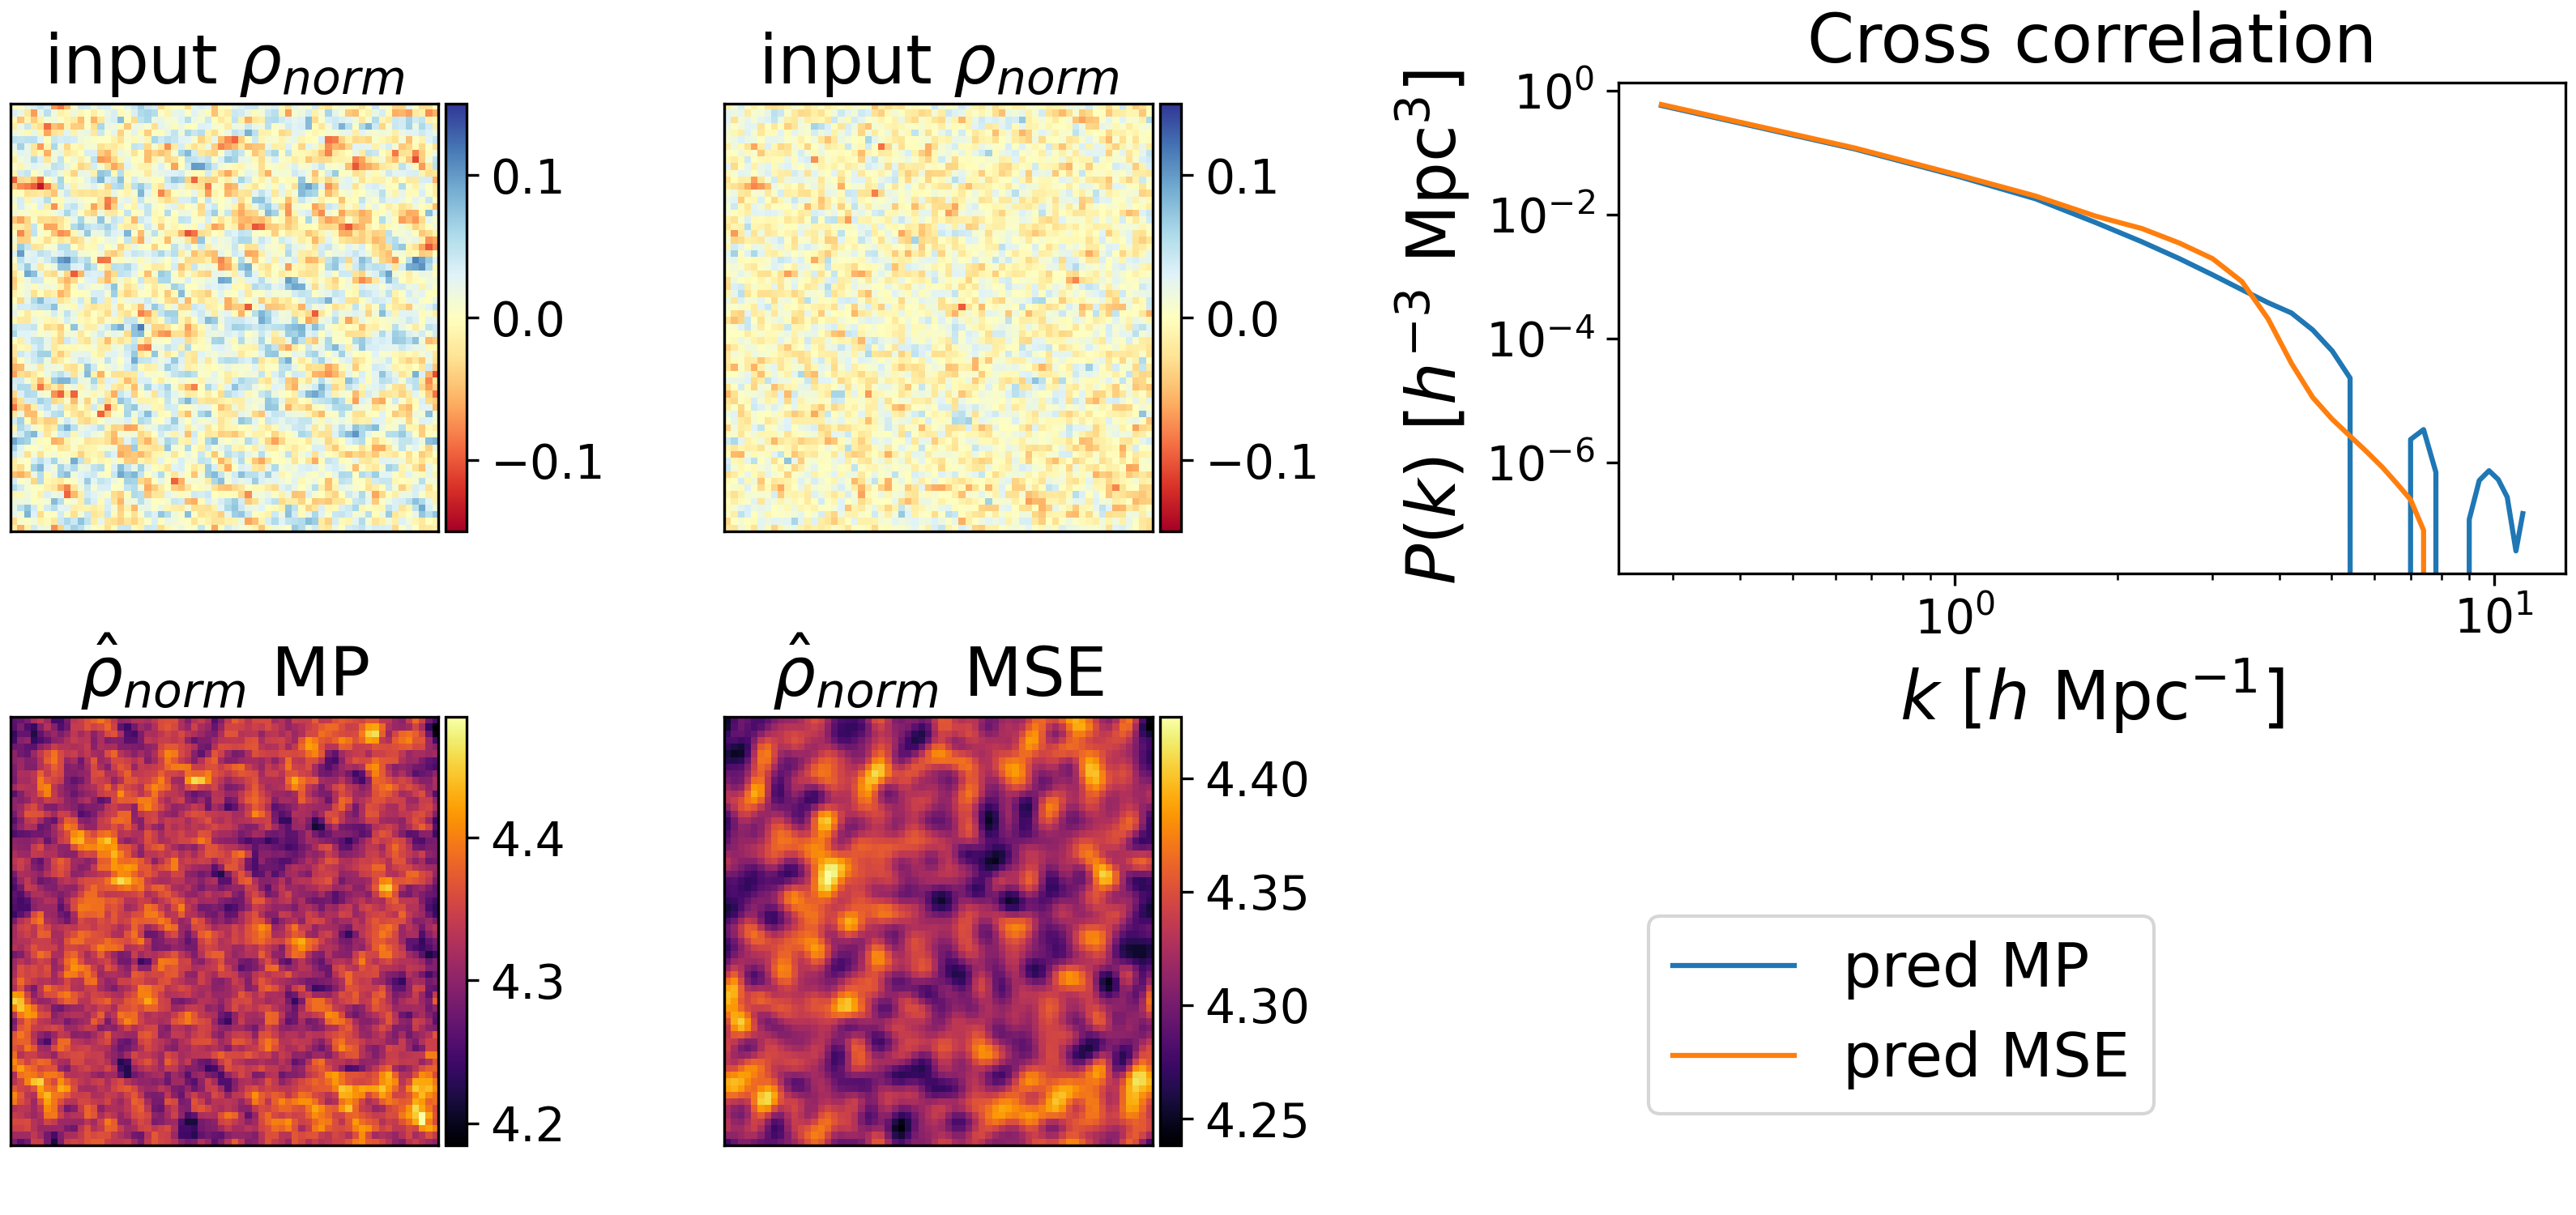
\includegraphics[width=0.8\linewidth]{img/compare_loss_correlation.png}
    \caption{Prediction from $z=19.2$ to $z=49$, compared with or without additional power loss term.}
    \label{fig:power-loss-corr}
\end{figure}

In the realm of the very small wavelengths, why the network still appears to be struggling. This shortcoming is likely rooted in those structures being less penalized in the loss term, as their original value is lower than the one from the loss term. Furthermore, the adaptive version of the FNO has fewer capabilities in the higher wavelength region, as the design of the architecture allocates less computing power towards higher wavelengths. Consequently, leading to an inability to generate structures that accurately reflect the power spectrum for very small structures. Another concern was, that the network is unable to generate the small structures due to an unavailability of sourcing such a Gaussian noise needed to generate the structures. Therefore, we have experimented with including a second  input channel composed of random Gaussian noise. Potentially, this channel could provide the network with a source for smaller-scale structures. However, the results were underwhelming and we have not further investigated the approach.


\subsubsection{Gravitational Potential Feature}

\begin{figure}[h]
    \centering
    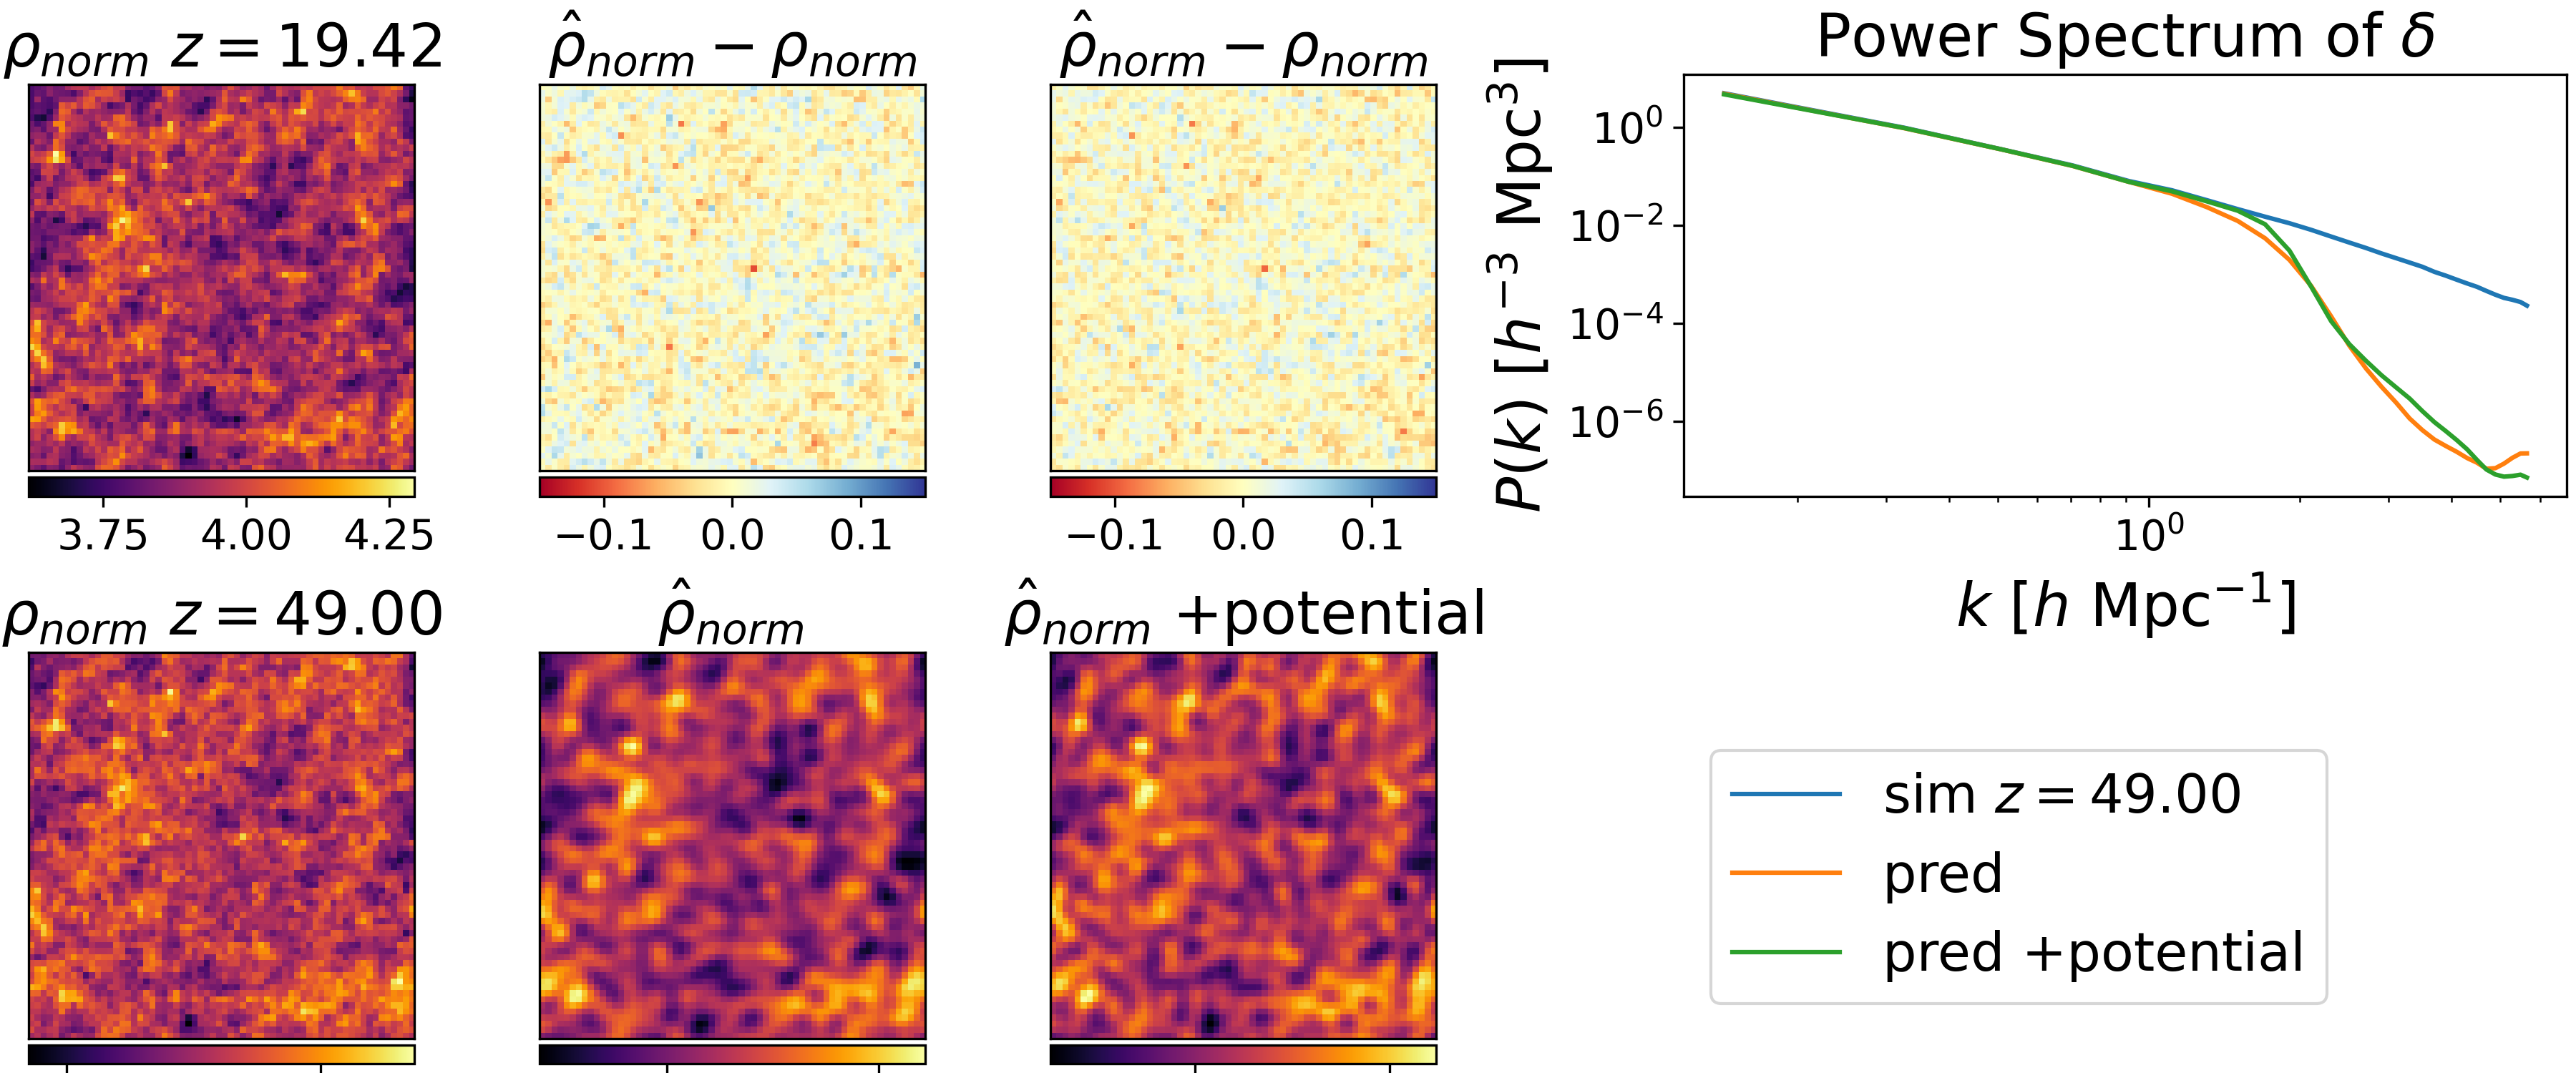
\includegraphics[width=0.7\linewidth]{img/compare_potential_4.png}
    \caption{Prediction from $z=19.2$ to $z=49$. Comparison of identical FNO networks trained on the density fields, with and without the potential as an additional input channel.}
    \label{fig:potential}
\end{figure}

As another way to possibly enhance the model's predictive skills, we propose enriching the input channels by integrating the gravitational potential field as an additional input feature. Note that adding another input is cheap, the number of trainable FNO network parameters will only increase by two times the hidden channels for each additional input channel. This added channel may enable the network to acquire a more profound understanding of the gravitational dynamics and spatial translations involved. The effects result in a slight improvement that is visually barely noticeable, as observable in figure \ref{fig:potential}. The network, which is trained with the input including the potential field, seems to be able to predict slightly smaller structures, than the other one. To conclude, the added gravitational potential channel does not improve the results enough in order for the idea to be persecuted further.



\subsection{Large Dataset Training}

So far we have performed all tests and experiments on the small dataset. Before moving on with more advanced autoregressive training schemes, we train the neural network on the large datasets. The large dataset offers twice the number of grid elements in each dimension, resulting in $2^3 = 8$ more grid elements. Furthermore, we ran three times more simulations to create it. Overall, leading to a significantly increased information quantity. In this section, we test whether training on the large dataset improves the predictive powers of the network. We leverage an adapted FNO with 4 layers and 16 channels. We train on the large dataset, where we downscale the distributions from $256^3$ to $128^3$ using cubic spline interpolation. This is necessary as we are otherwise unable to fit a single sample, even with a batch size of one, on the memory of the available GPU.  For the first time, we trained a network to predict the full-time range, thats is going from $z=0$ to $z=49$. Surprisingly, the network is capable of predicting the very large structures as reflected in subfigure (a) from figure \ref{fig:large}.

\begin{figure}[h]
\centering
\subfloat[Results from network trained on the range of $z=0$ to $z=49$.]{\label{fig:large-A}
\centering
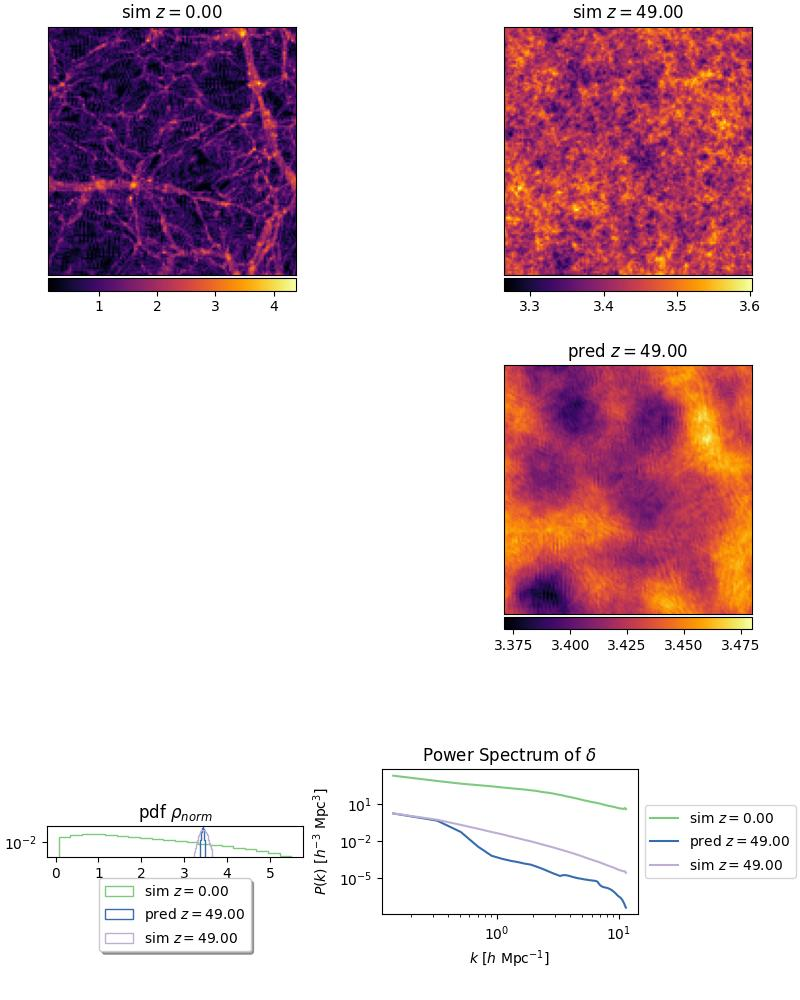
\includegraphics[width=0.45\linewidth]{img/large_z0_to_z49(1).jpg}
}
%no space
\hfill
\subfloat[Results from network trained on the range of $z=4.25$ to $z=49$.]{\label{fig:large-B}
\centering

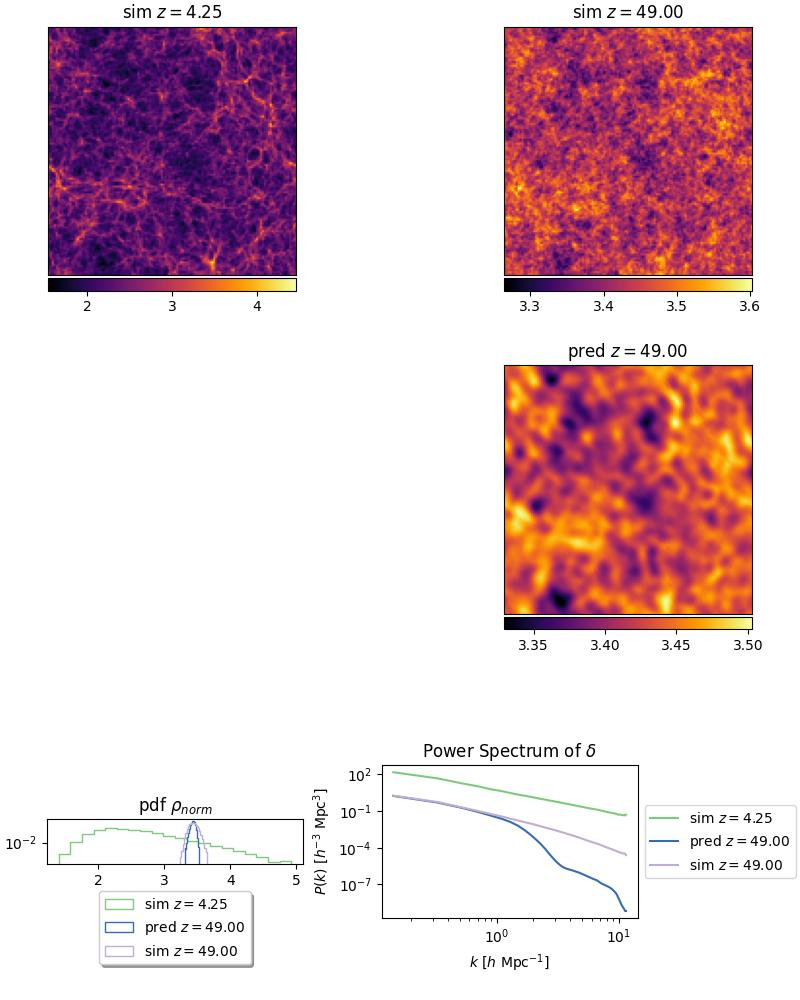
\includegraphics[width=0.45\linewidth]{img/large_z4_to_z49.jpg}
}

\caption{Training and prediction on large dataset.}
\label{fig:large}
\end{figure}

Interestingly, the power spectrum appears to drop less drastically on smaller wavelengths (higher modes). A similar trend can be observed on a model trained on the range $z=4.25$ to $z=49$, as seen in subfigure (b) from figure \ref{fig:large}. Here the power spectrum follows the ground truth power spectrum accurately until it starts to fall off for the higher modes. This reflects once again how training over larger times-spans is a harder prediction task, and a correlation between the scale of the predicted structures and the size of the time-span. We conclude, that the training of the network benefits from a larger dataset, since on the small dataset, training a model to predict from $z=0$ to $z=49$ resulted in almost no convergence. The exact correlation between the dataset size and training convergence is being increasingly investigated for neural network training across the board \citep{kaplan2020scaling}, where a lot of evidence points towards a linear relationship between the model accuracy and the combined parameters of compute time, dataset size and network size. The above relationship is said to be linear only if all three parameters are increasing simultaneously, and necessarily needs to converge to a non-linear relation before reaching completely accurate predictive capabilities.


\subsection{Auto-regressive Predictions}

\begin{figure}[h]
    \centering
    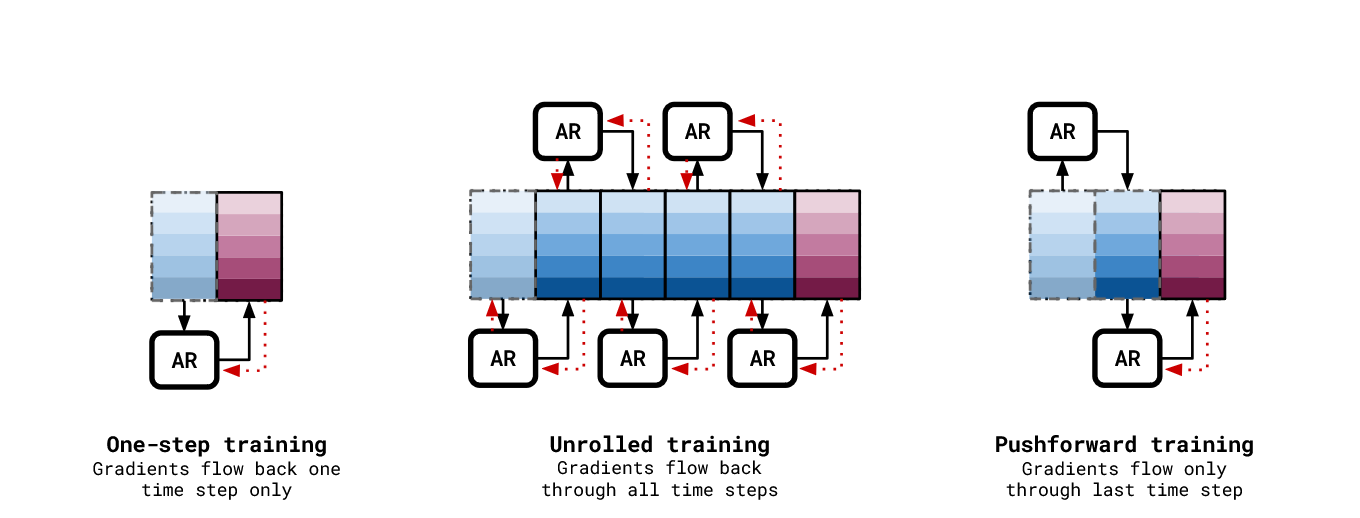
\includegraphics[width=0.75\linewidth]{img/schemes.png}
    \caption{Different training schemes. Figure from \cite {brandstetter2022message}.}
    \label{fig:schemes-training}
\end{figure}


Previously, we have observed how training and inference perform better when the time interval between the input and output of the neural network is smaller. Hence, a logical thing is to split the prediction into multiple smaller time-steps, similarly to a numerical time integration like PKDGRAV3 does. This is a very common approach in surrogate training for non-steady state problems such as fluid simulations \citep{li2020fourier}. In literature, such a chained prediction is commonly termed as autoregressive training. Recall, our original goal was to learn a network $\mathbf{f}$ that is capable of the following prediction

\begin{equation}
\label{goal-2}
    \mathbf{f}(\mathbf{x}(i, t_{n})) \approx \mathbf{x}(i, t_{0}).
\end{equation}

In an autoregressive setting, we call the network $\mathbf{f}$ recursively, meaning the output of the network is fed back into the network. Hence, the goal becomes

\begin{equation}
\label{goal-rec}
    \mathbf{f}_{n-1} \circ \mathbf{f}_{i-1} \circ \dots \circ \mathbf{f}_0(\mathbf{x}(i, t_{n}))\bigr) \approx \mathbf{x}(i, t_{0})
\end{equation}

where we recursively execute $n$ calls to $\mathbf{f}$. Here $\mathbf{f}_i = \mathbf{f}_j$ meaning all networks and their corresponding parameters are identical. There are a multitude of different training schemes available that have been explored in academia where the most simple one is the one-step training procedure, which applied to our problem setup translates to the loss function 

\begin{equation}
    L = \sum_{\mathbf{x} \in  \Omega} \Biggl(\mathbf{f}(\rho(\mathbf{x}, t_{i})) - \rho(\mathbf{x}, t_{i+1})\Biggr)^2.
\end{equation}

Here the loss is computed for the i-th step of the complete autoregressive prediction. Usually, we adapt the loss to include all $n$ steps to become


\begin{equation}
\label{step}
    L_{step} = \sum_{i \in \{0, \dots n\}}\sum_{\mathbf{x} \in 1 \Omega} \Biggl(\mathbf{f}_i(\rho(\mathbf{x}, t_{i})) - \rho(\mathbf{x}, t_{i+1})\Biggr)^2.
\end{equation}

We denote the above loss, and its subsequent neural network training as stepwise training, it can also be seen as an illustration in \ref{fig:schemes-training}. A disadvantage of the stepwise learning procedure is that the network does not learn to deal with accumulating errors that are present when the network called recursively. Another training scheme is the unrolled training, where the entire chain of chained neural networks is evaluated, the loss is evaluated and then back propagated through the entire chain. The corresponding MSE loss function is 

\begin{equation}
\label{seq}
    L_{seq} = \sum_{i \in \{0, \dots n\}}\sum_{\mathbf{x} \in \Omega} \Biggl(\mathbf{f}_{i-1} \circ \mathbf{f}_{i-2} \circ \dots \circ \mathbf{f}_0 (\rho(\mathbf{x}, t_{i})) - \rho(\mathbf{x}, t_{0})\Biggr)^2.
\end{equation}

Sequential training is illustrated in figure \ref{fig:schemes-training}. Finally, there is push forward training, where the loss function is equivalent to the $L_{seq}$ loss function; however, the gradient is only propagated through the very last step. Besides some advantages to convergence \citep{brandstetter2022message}, having to pull the gradient only over a single iteration of the solver drastically reduces the memory footprint of the AD over the program. As we have learned in section \ref{ad}, the only feasible AD method, that is backward mode differentiation, is required to store all inputs of all atomic operations in the function that is to be differentiated. In this case, the unrolled training procedure means all $n$ recursive invocations of the neural network $\mathbf{f}$ can be considered one large function $\mathbf{g}$ that is 

\begin{equation}
    \mathbf{g} = \mathbf{f}_{n-1} \circ \mathbf{f}_{n-2} \circ \dots \circ \mathbf{f}_0.
\end{equation}

Therefore push forward training drastically reduces the memory footprint of the training procedure. Another notable training scheme is curriculum learning, where the number of training steps is gradually increased over the course of the training \citep{krishnapriyan2021characterizing}, increasing the convergence speed of the training process. Unfortunately, in our experience, using a single network that is recursively applied to predict the underlying data did not work. With curriculum learning, the network is capable of learning a single step, but as soon as the recursive training procedure for multiple time steps starts, the performance of the network drastically decreases. We think the time aggregated density data is especially tricky to learn, as the dynamics at play are highly non-homogenous over time. In other words, initially linear effects are the dominant driver of the physics, which are then replaced by non-linear dynamics later on. One idea was to include a time embedding layers as an additional input channels. This would enable the network to know at which point in time its predictions are to be made. To achieve this, we extended the input channel size of the FNO by two and gave it the density field, the growth factor at the starting point of the time step and the endpoint of the prediction. However, even with this approach we were not successful. Before we go on with the solution that has worked for us, we would like to point out some advantages of the autoregressive approach. Overfitting is almost impossible. Because the task at hand can only be solved by understanding the actual dynamics, and not by memorization. Furthermore, the dataset size is increased by the number of time steps, potentially increasing the number of samples the network can be trained on without having to run more simulations. 

\subsubsection{Unique Network Parametrization}

\begin{figure}[h]
    \centering
    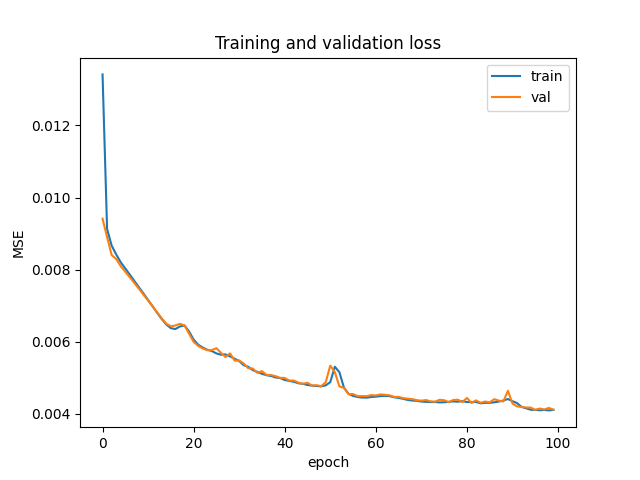
\includegraphics[width=0.9\linewidth]{img/training.png}
    \caption{Different training schemes for unique network parametrization. Here the blue boxes denote the sequence of ground truths, the orange boxes are the predictions, green is the loss and and purple denotes the parameters of the invidivual neural networks.}
    \label{fig:autoreg}
\end{figure}

In our case, however, we have resorted to unique network parametrization. That is we have identical neural network architectures for each timestep, but their learnable parameters are initialized and learned independently of each other. This approach is not autoregressive training, since we do not call the same function recursively, but instead we have a unique function for each time step. Everything we have stated before still holds, with minor differences. We now have $\mathbf{f}_i \neq \mathbf{f}_j$ and push forward training does not really make sense as it would only train the parameter of the very last network. Instead, we introduce a mixed mode training, where the loss is only evaluated on the very last iteration instead of the entire chain of predictions. The loss is then back propagated through the entire chain of networks, that is the loss is evaluated as

\begin{equation}
\label{mix}
    L_{mix} = \sum_{\mathbf{x} \in 1 \Omega} \Biggl(\mathbf{f}_i \circ \mathbf{f}_{i-1} \circ \dots \circ \mathbf{f}_0 (\rho(\mathbf{x}, t_{n})) - \rho(\mathbf{x}, t_{0})\Biggr)^2.
\end{equation}

We have found that training a network for several epochs using $L_{step}$ followed by a smaller number of epochs using $L_{seq}$ and $L_{mix}$ yields the best results. An illustration of the individual loss functions can be seen in \ref{fig:autoreg}. Gradients obtained by differentiating the $L_{seq}$ and $L_{mix}$ loss function are suffering from vanishing and exploding gradients problem because the loss needs to be propagated through the whole chain of networks \citep{thuerey2021physics}. We reduce contain the vanishing gradients problem by implementing gradient clipping as described in literature \citep{zhang2019gradient}. In a first experiment, we trained two networks, one network $\mathbf{f}_0$ is trained on the Redshift range 0 to 4.25, the other  $\mathbf{f}_1$ on 4.25 to 49. The time ranges are selected based on the learning from section \ref{timeintervals}, where we have observed, that learning ranges that are closer to $z=0$ is easier. While the redshift numbers might be deceiving, the second network  $\mathbf{f}_i$ learns a larger timespan than the first one. The network was trained for ten epochs using the $L_{step}$ loss and 5 epochs on each of the $L_{seq}$ and $L_{mix}$ loss. As the data, we opted for the large dataset, down scaled to a $128^3$ density field using cubic spline interpolation, with the same learning rate of $0.002$. The results are depicted in figure \ref{fig:multistep}. If we compare this to \ref{fig:large}, we can clearly observe how the power spectrum tends to fall off more slowly, which is also reflected by the presence of clearer smaller structures than in the direct prediction. 

\begin{figure}[h]
    \centering
    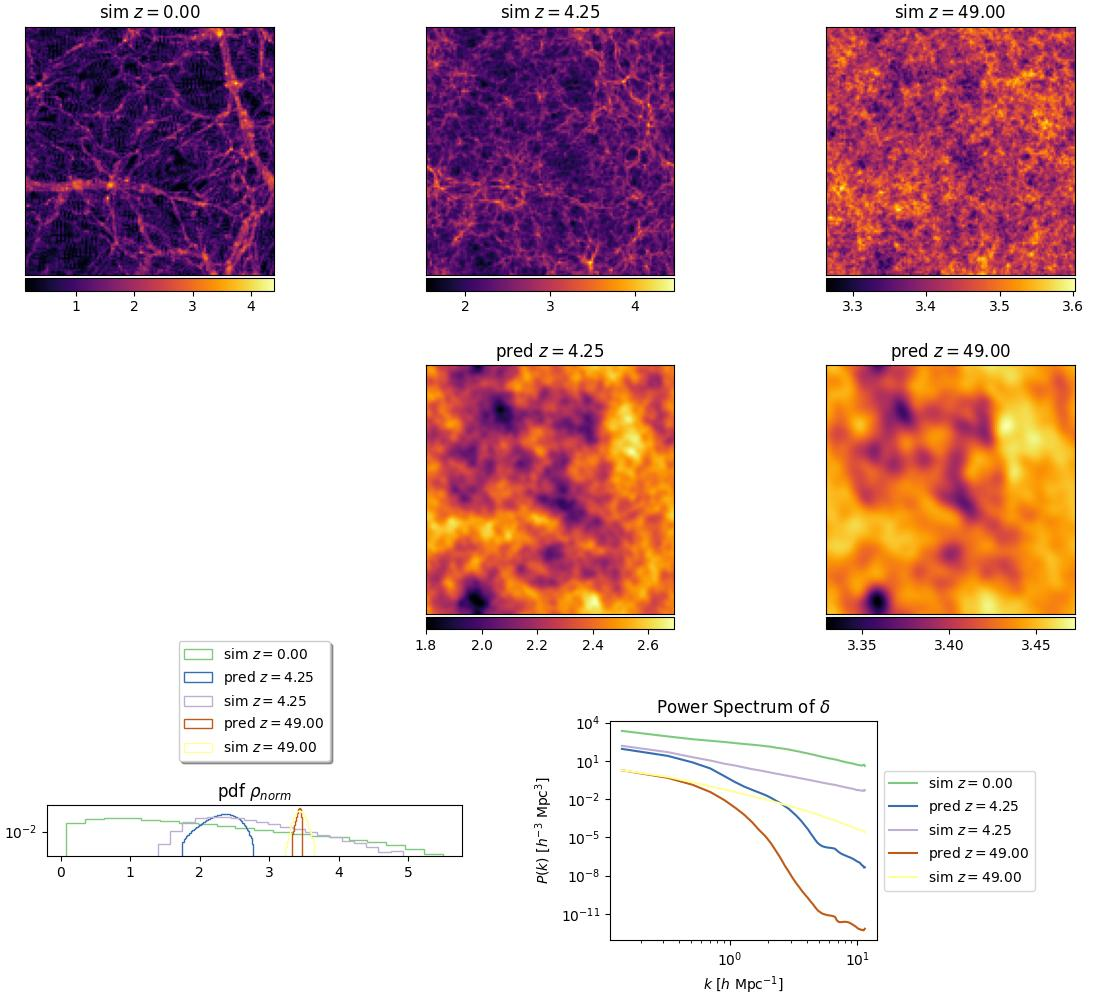
\includegraphics[width=0.9\linewidth]{img/multistep_large.jpg}
    \caption{Multistep Prediction on the large dataset using an FNO.}
    \label{fig:multistep}
\end{figure}


\subsubsection{Skip Connections}


\begin{figure}[h]
    \centering
    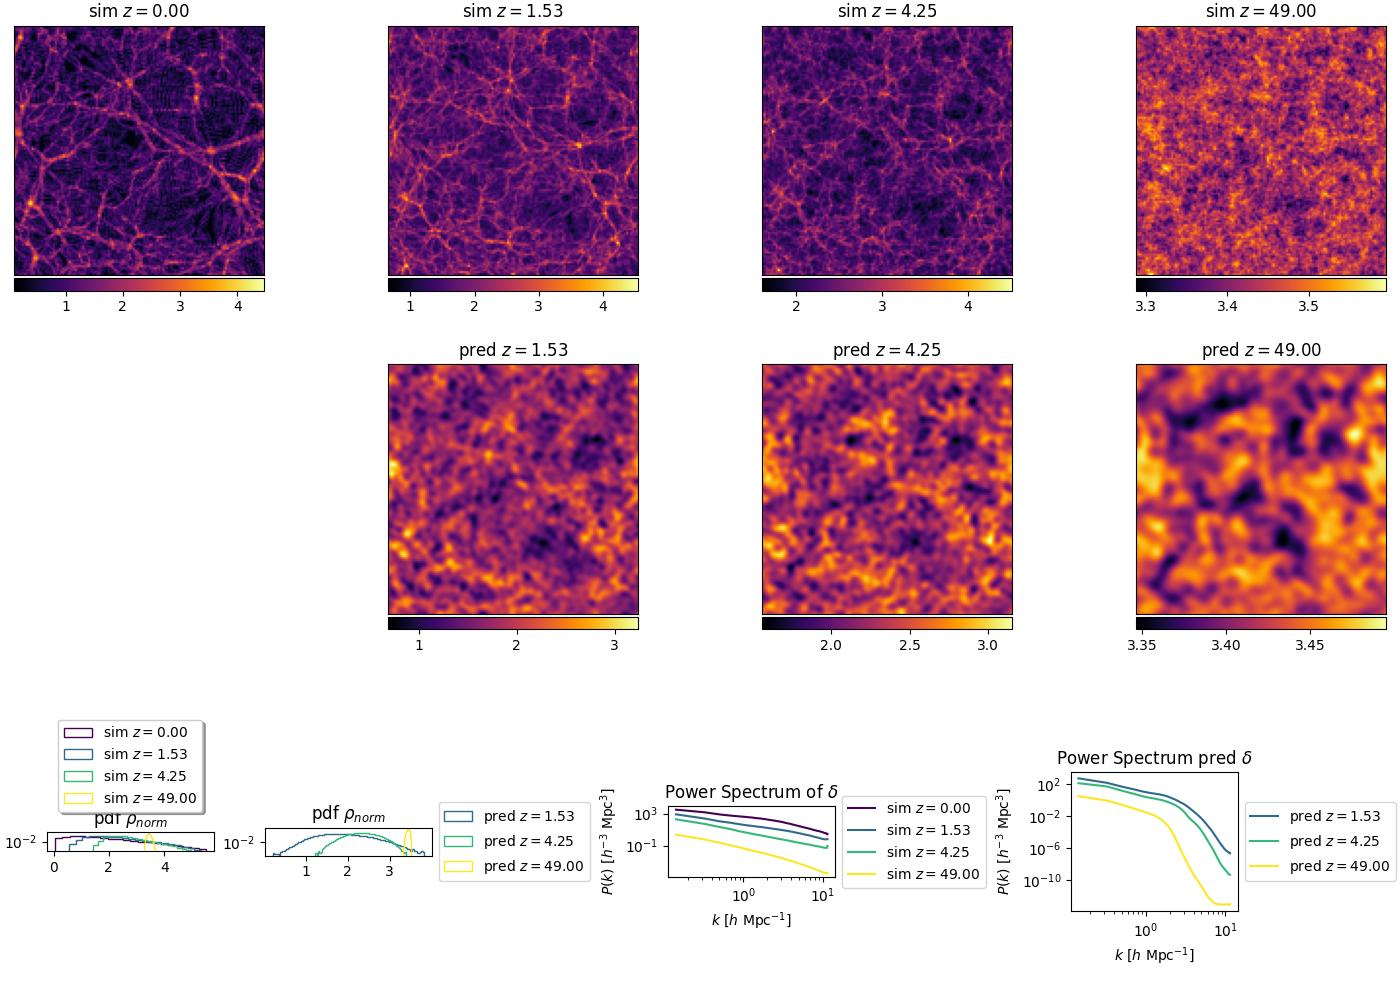
\includegraphics[width=0.9\linewidth]{img/prediction_sequential(1).jpg}
    \caption{Three-step prediction using an adaptive FNO with a three channel skip connections on the large dataset.}
    \label{fig:mss}
\end{figure}


Finally, we have tested another promising approach that is frequently used in neural networks and auto-regressive training, skip connections. The idea of skip connections is to have an alternative data pathway, where the data from previous timesteps can pass through unaltered.  This approach is inspired to current effort on applying FNO's in an autoregresive manner \citep{li2020fourier, gopakumar2023fourier}. A common approach is to train the FNO operators using similar step-wise loss functions as seen with the equation $L_{step}$ in a first training sequence. Then a Recursive Neural Network (RNN) is trained on the sequential loss function $L_{seq}$, where the parameters of the FNO are frozen. That means the RNN is responsible for correcting the accumulating errors. The setup helps to reduce the vanishing and exploding gradients problem. The architecture of RNN's almost always includes skip connections that can pass the data unaltered through the network. However, due to the time limitations of the thesis, we did not have time to implement a RNN and adapt the training regime. Instead, we borrow the idea of skip connections and just apply them to our FNO training.

Specifically, we increase the number of input and output channels for all networks $\{\mathbf{f}_i, \dots \{\mathbf{f}_{n-2}$ to $b$, representing the number of skip connection channels. The first network $\{\mathbf{f}_i$ has a single input channel and $b$ output channels, whereas the network $\{\mathbf{f}_i$ has $b$ input channels and one output channel. We then trained the network on the large dataset using the regular procedure to downscale the dataset to $128^3$ using cubic spline interpolation. We used $b=3$, meaning 3 skip connections. Furthermore, we added another intermediate step, meaning we used three unique neural networks $\mathbf{f}_0$, $\mathbf{f}_1$ and $\mathbf{f}_2$. Here network 0 predicts from $z=0$ to $z=1.53$, network 1 from $z=1.53$ to $z=4.25$ and finally network 2 from $z=4.25$ to $z=49$. The results are depicted in figure \ref{fig:mss}. We can observe the way the power spectrum falls off later, and we can make out a lot more details in the predicted distribution. The results from the experiment with two and three uniquely parametrized networks hint towards a positive correlation between the number of unique networks and the training accuracy. However, this approach becomes unfeasible to train on a single GPU machine. Even with a powerful H100 NVIDIA GPU boasting 100 GB of GPU memory and a batch size of just one, we have hit the memory limit with this implementation. Splitting the prediction into more timestep would require either a multi GPU setup or advanced gradient check pointing techniques, as briefly described in section \ref{IC-opt}. 



\newpage
\section{Implementation}
\label{impl}

Due to the very mature machine learning ecosystem, we have decided to use Python for all implementations. A crucial component for any project involving gradient-based optimization and consequently machine learning, is a library that supports storage, mathematical operations, and automatic differentiation on multidimensional arrays—ideally offering vectorization and GPU support. We have considered using Julia along with Enzyme, which can outperform all other automatic differentiation libraries  \citep{enzyme1, enzyme2, enzyme3}. However, after some preliminary experiments we found Enzyme to be time-consuming in practice, especially in an explorative setting as ours. With enzyme, the user is responsible for memory management of all variables during primal evaluation for the later usage for backward mode differentiation. The experiment is detailed in the Section \ref{diff-julia}.  
We have chosen {JAX} \citep{jax2018github}, as it provides greater flexibility than PyTorch while delivering similar performance \citep{dion_hafner_2021_5607491}. JAX, like other frameworks, leverages the open-source XLA (Accelerated Linear Algebra) library to compile the Python code, significantly boosting its performance. It boasts a wide range of features related to automatic differentiation, including taking gradients of gradients (Hessian), and exposing low-level primitives such as Vector Jacobian Products (VJP) and Jacobian Vector Products which are used for backward mode differentiation and forward mode differentiation. Still, interacting with the library remains relatively simple, as the user does not need to care about memory allocation as it is the case for libraries such as Enzyme \citep{NEURIPS2020_9332c513}.

For the implementation of standard neural network and helper classes, we use Equinox \citep{kidger2021equinox}. The main advantage of Equinox over the more popular JAX-based library Flax \citep{flax2020github} is its use of PyTrees to store model definitions. This means that learnable parameters are standard python class attributes. To compute the gradient with respect to a python object, equinox provides filter functions which traverse the PyTree and identify all {JAX} arrays, which are then traced and made differentiable using the AD capabilities of JAX. This approach offers greater flexibility and is a paradigm currently being adopted by Flax. We use Optax for its implementations of standard gradient-based optimization algorithms \citep{deepmind2020jax}, such as Adam \citep{kingma2014adam}.

Given the large volume of data we are processing, an efficient data-loading pipeline is crucial for reasonable training times and consequently rapid design iterations of the neural networks and the entire pipeline while development. We have selected NVIDIA DALI (Data Loading Library), which is capable of loading and applying common transformations to 3D tensors. In our case, we primarily rely on its CUDA accelerated rescaling capability, allowing us to downscale the 3D tensors using bicubic interpolation for model prototyping on smaller datasets. Furthermore, NVIDIA DALI data loaders enable efficient multiprocessor data loading and batching. Finall, to increase the robustness of our code, unit tests for all essential functions, models and training procedures are implemented with the Pytest Framework \citep{pytestx.y}.

While implementing the code for this thesis, we have noticed a lack of differentiable primitives that can be leveraged for predictions and optimizations in cosmology. Therefore, we have abstracted a few functions that have been implemented during the creation of the thesis and collected them in a python package. Some of the functions that are part of the package are not used for the training and inference of the thesis; however, they were crucial during the exploration stage. We have now released a python library named \textit{cosmax}, which is a combination of the two words cosmology and {JAX}. It is available from {PyPi} and can be installed by running the command {pip install cosmax} in any Python environment. The complete API is described on the webpage https://andrinr.github.io/cosmax/ and the source code is available under the MIT licence on github with URL https://github.com/andrinr/cosmax. 

\subsection{Model Serialization}

To compare and keep track and ensure reproducibility of hundreds of models trained on different datasets with varying hyperparameters and data pipeline configurations, we have implemented a comprehensive model and data loading serialization scheme. The python script responsible for orchestrating the training workflow, take as an argument a .yaml configuration file as seen in table \ref{table:config}.


\renewcommand{\arraystretch}{1.2}
\begin{table}[h!]
\small
\centering
\begin{tabular}{||l l l||} 
 \hline
 Variable & Type & Description \\ [0.5ex] 
 \hline\hline
 \multicolumn{3}{||c||}{\textbf{Dataset}} \\
 \hline
 grid\_dir & str & Directory where grid data is stored. \\ 
 input\_grid\_size & int & Size of the input grid for model training. \\ 
 grid\_size & int & Size of the grid used for making predictions. \\ 
 file\_index\_stride & int or list[int] & Stride of file indices used during processing. \\ 
 file\_index\_steps & int & Number of sequential files read during training. \\ 
 file\_index\_start & int & Initial index from which files are read. \\ 
 total\_index\_steps & int & Total number of index steps available in the dataset. \\ 
 normalizing\_function & str & The function used to normalize input data. \\ 
 flip & bool & Determines whether to flip the time axis of the data. \\ 
 \hline
 \multicolumn{3}{||c||}{\textbf{Training}} \\
 \hline
 include\_potential & bool & Indicates if potential data is included as an input channel. \\ 
 sequential\_skip\_channels & int & Number of channels skipped in sequential mode. \\ 
 stepwise\_epochs & int & Number of epochs dedicated to stepwise training. \\ 
 mixed\_epochs & int & Number of epochs allocated to mixed training approaches. \\ 
 sequential\_epochs & int & Epochs spent for training sequentially across steps. \\ 
 unique\_networks & bool & States if each timestep is learned by distinct networks. \\ 
 learning\_rate & float  & Rate at which the model adjusts weights during training. \\ 
 model\_dir & str & Directory where trained models are stored. \\ 
 model\_type & str & Specifies the neural network model type used. \\ 
 activation & str & The activation function employed in the network. \\ 
 \hline
 \multicolumn{3}{||c||}{\textbf{FNO parameters}} \\
 \hline
 fno\_modes & int & Number of modes used in the Fourier Neural Operator. \\ 
 fno\_input\_channels & int & Channels fed into the FNO model as input. \\ 
 fno\_hidden\_channels & int & Hidden channels within the FNO model structure. \\ 
 fno\_output\_channels & int & Channels output from the FNO model. \\ 
 fno\_n\_layers & int & Number of layers comprising the FNO model. \\ 
 fno\_increasing\_modes & bool & Whether the FNO uses a setting with increasing modes. \\ 
 \hline
 \multicolumn{3}{||c||}{\textbf{UNet parameters}} \\
 \hline
 unet\_input\_channels & int & Number of input channels of the UNet. \\ 
 unet\_hidden\_channels & int & Number of hidden channels in the UNet architecture. \\ 
 unet\_output\_channels & int & Number of output channels produced by the UNet. \\ 
 unet\_num\_levels & int & Number of resolution levels in the UNet model. \\ 
 \hline
 \multicolumn{3}{||c||}{\textbf{Cosmos}} \\
 \hline
 box\_size & int & Physical size of the simulation box, often in Megaparsecs/h. \\ 
 num\_particles & int & Total number of particles in the simulation. \\ 
 omega\_M & float & Density parameter for matter in the cosmological model. \\ 
 omega\_L & float & Density parameter for dark energy in the cosmological model. \\ 
 \hline
\end{tabular}
\caption{Configuration parameters for the volumetric training pipeline.}
\label{table:config}
\end{table}

The training pipeline is set up, such that we can provide it with a variable named grid\_dir in the config file, which denotes the root directory of the density field datasets. A root directory then contains several subdirectories, whereas each contains a simulation run with density fields stored as binary files. Naturally, the number of files in such a directory depends on the specific settings provided to the simulation software of choice. 
The data loader then discovers and sorts by name all files with each simulation run. The loader will then read the file which is at the index denoted by  file\_index\_start first. The loader then takes file\_index\_steps with a stride of file\_index\_stride. Here the flip parameters denotes the sign of the individual steps, meaning that if flip is enabled, the steps are taken multiplied with a negative sign, meaning we start from a file later in order and go back to files earlier in order. Alternatively, the user can also provide a list for the value of file\_index\_stride, leading to specific strides for each step. As soon as we set file\_index\_steps to a value greater than one, the training becomes auto-regressive. Meaning the output of the neural network is repeatedly fed back into itself, or if the parameter unique\_networks is enabled, an identical network with unique parameters. unique\_networks ensures that for each step, a model with a unique set of parameters is initialized and trained. This enables model specification for a given time range, and is especially useful in tasks where the underlying dynamics are non-uniform across the timeline. In the parameters we can also individually set the number of mixed, sequential and stepwise epochs, where the corresponding loss function are implemented as described in formulas \ref{step}, \ref{seq} and \ref{mix} and are executed in the order they appear here in the text.

After a training run is completed, the entire config file, the model weights and training statistics are stored in a single binary file. This enables us to easily read such a file, perform tests on it and know of the specifics of the relevant training pipeline. We have set up several scripts, which take a folder of different training runs and visually compare them against each other.

\subsection{Parallelization}

Generally we use vectorized operations as exposed by {JAX} whenever possible. In {JAX} all such vector operations can be executed on the CPU or the GPU, depending on the hardware availability \citep{jax2018github}. To further accelerate the training process, we vectorize the training of a batch using the `vmap` function. Additionally, we exploit the Just-In-Time (JIT) compilation capabilities of {JAX} wherever applicable. To enhance JIT compilation time, we utilize JAX's `fori` loops instead of native Python `for` loops. Finally, whenever feasible, we replace sequential for loops with parallel scans, which also contributes to faster JIT compilation.


\subsection{Differentiable Power Spectrum}

Since a differntiable power spectrum implementation, does to the best of our knowledge, not exist so far, and its implementation is rather complicated, we want to explain this part of our code in detail.

\begin{lstlisting}[language=Python]
class SpectralOperation:
    k_mag = jax.Array
    frequencies : jax.Array
    elements : int
    size : float
    nyquist : int

    def __init__(self, elements : int, size : float = 1.0):
        self.elements = elements
        self.size = size

        self.frequencies = jnp.fft.fftfreq(
            elements, 
            d=self.size / self.elements
        ) * 2 * jnp.pi
            
        self.real_frequencies = jnp.fft.rfftfreq(
            elements,
            d=self.size / self.elements
        ) * 2 * jnp.pi

        kx, ky, kz = jnp.meshgrid(
            self.frequencies, 
            self.frequencies, 
            self.real_frequencies, 
            indexing='ij')
            
        self.k_mag = jnp.sqrt(kx**2 + ky**2 + kz**2)
\end{lstlisting}

The spectral operation is designed for Fourier space operations on square, real valued scalar fields with periodic boundary conditions. To initialize a {Spectral Operation} we pass it the number of elements, which is assumed to equal in dimension and the physical size of the domain in the desired unit of interest. We then use the built-in operations from {jax.numpy.fft} to obtain the frequencies in complex and real space and normalize them by passing the size divided by the number of elements as the parameter {d} which represents the grid voxel distance. At last, we scale them to radians in unit space. The above described operations are computed on lines 12 to 20 in the python code listing above. Next up, we compute the wavelength magnitude by constructing a 3D scalar field with the help of the meshgrid operation. Meshgrid takes an array for each dimension of the final 3D vector field, and repeats it across the other dimensions. This means the first array, which in that case are the complex Fourier frequencies, is repeated in the direction of the y and z axis and is then returned and captured in the {kx} array. Here, kx, ky and kz are each 3D scalar fields. We then compute the distance by computing the Euclidean distance of those three scalar fields and store in the variable {k\_mag}.



\begin{lstlisting}[language=Python]
class PowerSpectrum(SpectralOperation):
    bins : int
    index_grid : jax.Array
    n_modes : jax.Array

    def __init__(self, elements : int, bins : int, size : float = 1.0):
        super().__init__(elements=elements, size=size)
        self.bins = bins

        self.bin_edges = 
            jnp.linspace(0, self.k_mag.max(), self.bins + 1, endpoint=True)[1:]

        bins_pad = 
            jnp.pad(self.bin_edges, (1, 0), mode='constant', constant_values=0)
            
        self.k = (bins_pad[1:] + bins_pad[:-1]) / 2

        self.index_grid = jnp.digitize(
            self.k_mag, 
            self.bin_edges,
            right=False)

        self.n_modes = jnp.zeros(self.bins)
        self.n_modes = self.n_modes.at[self.index_grid].add(1)

    def __call__(self, delta : jax.Array) -> Tuple[jax.Array, jax.Array]:

        V = float(self.size ** 3)
        Vx = V / self.elements ** 3

        delta_k = jnp.fft.rfftn(delta, norm="backward")  
        delta_k = Vx * delta_k

        power = jnp.real(delta_k * jnp.conj(delta_k) / V)

        power_ensemble = jnp.zeros(self.bins)
        power_ensemble = power_ensemble.at[self.index_grid].add(power)

        power_ensemble_avg = power_ensemble / self.n_modes
        power_ensemble_avg =      
            jnp.where(jnp.isnan(power_ensemble_avg), 0, power_ensemble_avg)
    
        return self.k, power_ensemble_avg
\end{lstlisting}

The Power Spectrum class inherits the Frequency Operation class using standard python class inheritance. Subsequently, the frequencies and the {k\_mag} field are available here. The main goal of the power spectrum is to get the amplitude of the density field for each wavelength vector length and then assign them to specific number of bins. First, we compute the values of the edges of the bins with the {linspace} function, which linearly distributes a desired number of values between a minimum and a maximum as applied on line 10 in the above code. Afterward, we compute the center values of the bins, that is, the average of the value of its left edge and the right edge. This can be achieved in a vectorized way by first padding the array at index zero by inserting another value of zero. Then we add up the left and right edges with an elementwise sum and finally compute the average by dividing by two (line 13). Note that the above is required to be done without using for loops, as for loops are not backwards differentiable \citep{jax2018github}. Now, we compute the number of elements in the Fourier transformed density field that are associated with a specific mode. This can be achieved with the digitize function, which bins the values from its first input variable, in our case the magnitude, to the bins designated by the right edges as specified with the second input (line 18). The function then returns the index of the corresponding bin for each entry in the first array, subsequently returning a 3D array. Ultimately, we count the number of elements that are assigned to each bin, using a notation that is unique to JAX. All of the above operations are done in the initialize array, as they are identical for each invocation of the power spectrum, as long as the density field size and the number of bins remain identical. This design increases computing time as the values can be reused. The {jnp.digitize} uses a binary search to perform the desired action, and should therefore not be underestimated in its performance on the runtime.
When the power spectrum is executed for a specific density field, we call the call functions. That is, we compute the physical volume of the density field and the physical volume of a grid cell in the density field on lines 28 and 29. We then transform the density field into Fourier space with the fast Fourier Transform and multiply it with the physical cell volume. We then compute the amplitude of the complex value and normalize it by dividing by the volume, as seen on line 34. The normalizations are standard practice to obtain the power spectrum for density fields in cosmology \citep{murray2018powerbox}. We then sum the amplitudes for each corresponding bin, normalize them by dividing through the total number of fields associated with each bin, and replace undefined values with zero on lines 35 to 41. The undefined values can be introduced with bins that have no fields assigned to them. Finally, we can return the magnitudes and their respective normalized amplitudes. In figure \ref{fig:powerspectrum} we can observe the resulting power spectrum as applied to an overdensity field. 

\begin{figure}
     \centering
     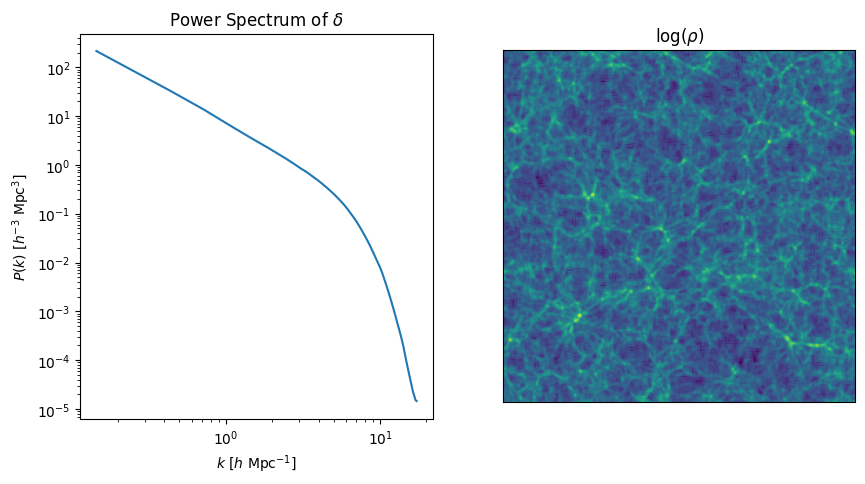
\includegraphics[width=0.75\linewidth]{img/power.png}
     \caption{Power spectrum computed on an overdensity field at $z=49$.}
     \label{fig:powerspectrum}
 \end{figure} 
 
\subsubsection{Performance}

When measuring the execution time of the power spectrum calculation, our implementation is faster than another library called {PowerBox} \citep{murray2018powerbox}, even without gpu acceleration. The results can be seen in figure \ref{fig:cosmax-bench}. This is surprising, since {PowerBox} is based on FFTW, a highly optimized C library for Fourier Transforms \citep{frigo1999fftw}. We have excluded the warm-up execution time of the {JAX} JIT compiler, which includes optimization and compilation of the function. For this reason, you might not see a speedup but a slowdown if {PowerBox} is replaced with our code naively. Generally speaking, the performance gains of our implementation are felt, when the power spectrum calculations are done repeatedly, e.g., in optimization loops.

\begin{figure}[h]
    \centering
    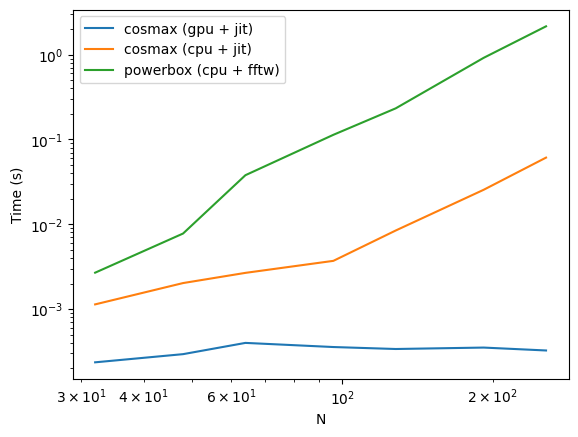
\includegraphics[width=0.5\linewidth]{img/benchmark.png}
    \caption{Cosmax power spectrum benchmark.}
    \label{fig:cosmax-bench}
\end{figure}


\subsection{3D FNO}

There are existing implementations of 3D FNO's for {PyTorch, however in our case we needed to translate it to {JAX} \cite{jax2018github} and the neural network library equinox \citep{kidger2021equinox}. We have used two GitHub repositories as reference implementations, where one of them is the original FNO implementation \citep{machinelearningsimulation, kossaifi2024neural}. The Fourier Neural Operator is divided into three classes, the Spectral Convolution, the Fourier Layer and the FNO class. We will describe only the Spectral Convolution as it is the most essential and challenging operation to implement. We define the {SpectralConvolution} class, which inherits from the equinox base module. It is initialized by setting the number of modes, the number of channels and a random key.  We then compute a scaling factor (line 15) as suggested in, \citep{li2020fourier} that is then used to initialize the weights of the complex matrices. The complex matrices are initialized as eight separate real valued matrices. We implement eight instead of one to omit applying a Fourier space shifting operation. You can observe in figure \ref{fig:shifting} that instead of keeping the large center section of the density field, we keep all corners of the real spaced values, that is two in the case of a 2D field and 4 corners in the case of a 3D field. Furthermore, we need to perform a complex multiplication; hence, we populate the weight matrices with real valued and complex valued parameters. 

\begin{figure}[h]
    \centering
    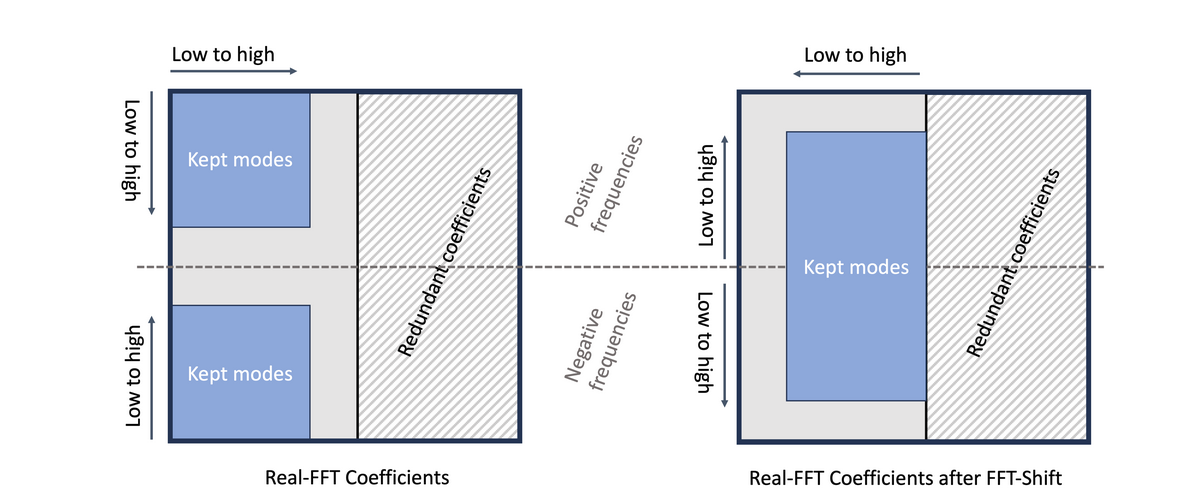
\includegraphics[width=0.75\linewidth]{img/image.png}
    \caption{Spectral Convolution without and with Fourier Space Shifting. Figure from  \cite{kossaifi2024neural}.}
    \label{fig:shifting}
\end{figure}

The eight weight matrices are initialized on lines 17 to 32 of the code listing below. Note that each weight matrix is of shape $c \times c \times m \times m \times m$, where $m$ denotes the number of kept modes, simply denoted as modes int the code and $c$ the number of channels, denoted as {n\_channels} in the code. Recall the definition of the spectral convolution

\begin{equation}
\label{spectral-conv}
    (u \ast c)[\mathbf{v}, c] = \sum_{i \in \{0, \dots, c_{in}\}} \mathcal{F}^{-1}\Bigl(\mathcal{F}(u)[\mathbf{k}, i] \cdot \mathbf{V}[\mathbf{k}, c, i] \Bigr).
\end{equation}

The matrix multiplication $\mathcal{F}(u)[\mathbf{k}, i] \cdot \mathbf{V}[\mathbf{k}, c, i]$ is implemented using the {einsum} function from {JAX} as seen on line 34 and 35, where a and b are both complex matrices. Here, instead of having a three-dimensional vector $\mathbf{k}$, we access the array using the individual vector components x, y and z. The indices $i$ and $c$ are exactly as in the equation \ref{spectral-conv}, just that the matrices are arranged differently. Meaning the channels are indexed in the leading dimensions. 


\begin{lstlisting}[language=Python]
class SpectralConvolution(eqx.Module):
    modes : int
    weights_real : list[jax.Array]
    weights_imag : list[jax.Array]

    def __init__(
            self, 
            modes : int,
            n_channels : int,
            key):
        
        self.modes = modes
        keys = jax.random.split(key, 8)
        
        scale = 1.0 / (n_channels ** 2)

        self.weights_real = []
        self.weights_imag = []

        for i in range(4):
            real = jax.random.uniform(
                keys[i], 
                (n_channels, n_channels, modes, modes, modes),
                minval=-scale, maxval=scale)
            
            imag = jax.random.uniform(
                keys[i + 4], 
                (n_channels, n_channels, modes, modes, modes),
                minval=-scale, maxval=scale)
            
            self.weights_real.append(real)
            self.weights_imag.append(imag)
        
    def complex_mul3d(self, a, b):
        return jnp.einsum("ixyz,icxyz->cxyz", a, b)
\end{lstlisting}

The actual operation is then applied by calling the instanced class. Here, we pass the original field as the unique input parameter $x$. The function then applies the Fourier transform on the relevant axes, which in our case excludes the very first axis, as it is reserved for the number of channels (line 4, code below). The Fourier transform as implemented in {JAX} automatically executes in parallel for all axes that are not passed as an argument.  Then for each of the four corners, we build the complex matrix and assign it to the weights variable as seen on lines 8, 16, 24 and 32. Then we perform the complex multiplication, by slicing the input at the correct corner locations and multiplying it with the weights' matrix as seen on lines 9, 17, 25 and 33. Finally, we transform the resulting array back into real space and return it as seen on line 40.

\begin{lstlisting}[language=Python]
 def __call__(self, x : jax.Array):
    N = x.shape[1]

    x_fs = jnp.fft.rfftn(x, s=(N, N, N), axes=(1, 2, 3))

    out_fs = jnp.zeros_like(x_fs)

    weights = self.weights_real[0] + 1j * self.weights_imag[0]
    out_fs = out_fs.at[:, :self.modes, :self.modes, :self.modes].set(
        self.complex_mul3d(
            x_fs[:, :self.modes, :self.modes, :self.modes],
            weights
        )
    )
    
    weights = self.weights_real[1] + 1j * self.weights_imag[1]
    out_fs = out_fs.at[:, -self.modes:, :self.modes, :self.modes].set(
        self.complex_mul3d(
            x_fs[:, -self.modes:, :self.modes, :self.modes],
            weights
        )
    )
    
    weights = self.weights_real[2] + 1j * self.weights_imag[2]
    out_fs = out_fs.at[:, :self.modes, -self.modes:, :self.modes].set(
        self.complex_mul3d(
            x_fs[:, :self.modes, -self.modes:, :self.modes], 
            weights
        )
    )
    
    weights = self.weights_real[3] + 1j * self.weights_imag[3]
    out_fs = out_fs.at[:, -self.modes:, -self.modes:, :self.modes].set(
        self.complex_mul3d(
            x_fs[:, -self.modes:, -self.modes:, :self.modes], 
            weights
        )
    )

    return jnp.fft.irfftn(out_fs, s=(N, N, N), axes=(1, 2, 3))
\end{lstlisting}




\newpage
\section{Conclusion}

In this thesis, we explored the feasibility of using Fourier Neural Operators (FNOs) to directly predict the initial conditions of dark matter simulations from their final states. Our work addressed the inverse problem of reconstructing the primordial density field at high redshift $z=49$ from evolved distributions at lower redshifts. We're leveraging deep learning techniques to bypass the computational and numerical challenges of using gradient and gradient free optimization that is associated with traditional constrained initial condition predictions. In this thesis, we have conducted the following experiments:

\begin{itemize}
    \item Normalization Strategies: We identified the log growth normalization as critical for training stability and performance. This approach scales the density field by the linear growth factor and applies a logarithmic transformation, effectively balancing the dynamic range of high- and low-density regions while preserving cosmological relevance.

    \item Adapted FNO Architecture: We introduced an FNO variant with increasing Fourier modes across layers, enabling progressive refinement of predictions from large to small scales. This design improved accuracy compared to standard FNOs and UNets.

    \item Differentiable Power Spectrum: We developed a GPU-accelerated, differentiable power spectrum implementation, enabling physics-informed loss functions that penalize spectral deviations. While mixed results were observed, this tool provides a foundation for gradient-based optimization methods in cosmology, with or without neural networks. Additionally, our implementation drastically outperforms the state-of-the-art library for measuring the power spectrum from python. 

    \item Auto-regressive Training: We tested applied various training schemas to perform autoregressive training on the dataset. We were able to improve our results by using unique network parametrization for each time step, allowing skip connections and increasing the density of prediction models. However, challenges like vanishing gradients and memory constraints limited scalability.
\end{itemize}

The key finding of this thesis are:

\begin{itemize}
    \item Large-Scale Success, Small-Scale Struggles: The FNO excelled at predicting large-scale structures (low k-modes) but underperformed on small scales (high k-modes). This aligns with theoretical expectations, as small-scale structures are dominated by chaotic, nonlinear interactions.
    \item  Time Interval Sensitivity: Predictions degraded with longer time intervals between input and output. Auto-regressive approaches mitigated this but required careful balancing of step sizes and computational resources.
    \item  Dataset Scaling Benefits: Training on larger datasets, where both the density grid resolution and the number of simulations is increased, improved generalization, highlighting the importance of data volume.
\end{itemize}

The limitations and challenges are:

\begin{itemize}
    \item Memory and Compute Constraints: Training on high-resolution grids ($>128^3$) necessitated downsampling, sacrificing small-scale detail. Multi-GPU setups or gradient checkpointing could alleviate this in the future.
    \item Training Stability: Networks trained on long time long-time risked overfitting or divergence. Hybrid losses (e.g., combining MSE and power spectrum terms) showed promise but can mostly be considered a tool to generative add small-scale structure to the density field.
    \item  Physics Integration: While FNOs learned implicit dynamics, explicit physical constraints (e.g., Poisson’s equation) were not enforced, limiting physical consistency.
\end{itemize}

Future direction of this research could involve

\begin{itemize}
    \item  Graph-based Architectures: Graph Neural Network could  better handle particle-level dynamics.
    \item Observational Integration: Incorporating galaxy surveys or velocity data as additional input channels may improve training performance.
\end{itemize}

Our work demonstrates the potential of neural operators to accelerate cosmological inference, enabling rapid exploration of initial conditions consistent with observed structures. While challenges remain, this approach complements traditional Bayesian methods, offering a scalable framework for conditional IC prediction. 

\newpage

\begin{appendices}

\section{Exploratory Work in Differentiable Physics}

\subsection{Reverse Time Integration}
\label{rev-integration}

To produce the results as seen in image \ref{fig:error_inverse}, we have written a Julia code that does forward and reverse time integration for ODE's using the kick drift kick method \cite{hut1995building}. Its main components are functions responsible for the forward and the backward integration, which are identical apart from the reversed signs for the operations on lines 6, 8 and 12. Note that in Julia, vector operations are performed by adding a dot before an operation. That means {.+} results in an element wise or scalar addition of two vectors or a vector and a scalar.

\begin{lstlisting}[language=Julia]
# kick drift kick / leap frog
function kdk(particles::Particles, dt::Float64)
    # compute a(t)
    force = gravity(particles)
    # v(t + dt/2) = v(t) + a(t) * dt/2
    particles.vel .+= force .* dt / 2
    # x(t + dt) = x(t) + v(t + dt/2) * dt
    particles.pos .+= particles.vel .* dt
    # a(t + dt)
    force = gravity(particles)
    # v(t + dt) = v(t + dt/2) + a(t + dt) * dt/2
    particles.vel .+= force .* dt / 2
end

# reverse time integration
function rev_kdk(particles::Particles, dt::Float64)
    # compute a(t)
    force = gravity(particles)
    # v(t - dt/2) = v(t) - a(t) * dt/2
    particles.vel .-= force .* dt / 2
    # compute x(t - dt)
    particles.pos .-= particles.vel .* dt
    # a(t - dt)
    force = gravity(particles)
    # v(t - dt) = v(t - dt/2) - a(t - dt) * dt/2
    particles.vel .-= force .* dt / 2
end
\end{lstlisting}

The error is then measured by first integrating the particles forward in time, followed by a backward integration and finally the defect between the initial positions and the final integrated position is computed.

\begin{lstlisting}[language=Julia]
particles = Particles(n_particles, pos, vel)

for i in 1:n_steps
    kdk(particles, dt)
end

for i in 1:n_steps-1
    rev_kdk(particles, dt)
end

pos_end = Array(particles.pos)
error = sum((pos_ic .- pos_end).^2) / n_particles
\end{lstlisting}


\subsection{Differentiable Physics with Enzyme}
\label{diff-julia}

To figure out how mature the automatic differentiation libraries in Julia are and to test the feasibility of creating our own implementation of a differentiable solver, we started implementing a differentiable GPU N-Body code using Julia and Enzyme \citep{enzyme1, enzyme2, enzyme3}. Enzyme is said to outperform {JAX} and other AD libraries in specific cases, as the automatic differentiation happens in the compiler stage of the language.

\begin{figure}[h]
    \centering
    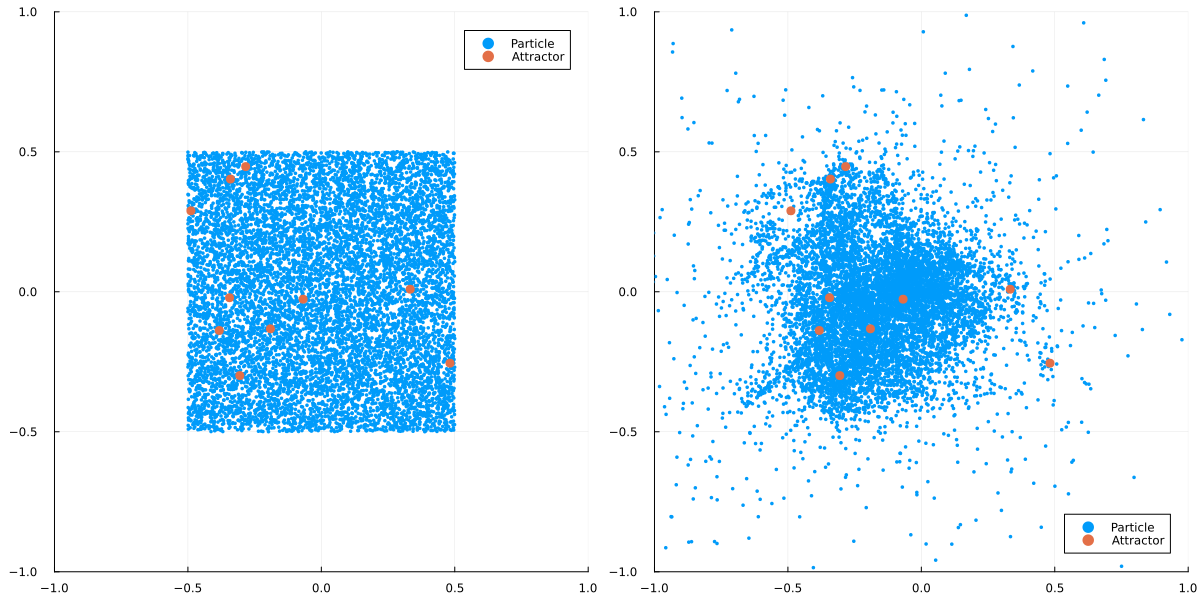
\includegraphics[width=0.9\linewidth]{img/particles.png}
    \caption{A particle system with ten attractors and, 10000 particles. The left plot shows the initial state, the right plot shows the state after a set number of iterations.}
    \label{fig:enzyme}
\end{figure}

A big disadvantage of Enzyme is the need to keep track of dual numbers and its memory requirements manually. This exposes a lot more of the AD functionality, which can increase the performance of a system when it is understood at a low level, however in projects such as this thesis this drastically increases the required development time. Before reaching a differentiable N-Body solver, we have stopped exploring the approach further. Nevertheless, we have learned something about Enzyme and produced some interesting plots such as figure \ref{fig:enzyme}.

\subsection{Adjoint ODE}
\label{adj-ode}

Inspired by the paper detailing a differentiable N-Body solver in {JAX} \citep{li2024differentiable}, we wanted to get a deeper understanding of adjoint methods. To this end, we have implemented an adjoint ODE solver learn the dynamics of an ODE on a single particle. All the theoretical information comes from the original paper about neural Ordinary Equations \cite{chen2018neural}. First, we solve the task using automatic differentiation.

Given the vector quantity of interest, $\mathbf{y}(t), t \in [0, T]$ we are considering a generic ODE of the shape:

\begin{equation}
\frac{d\mathbf{y}(t)}{dt} = f(\mathbf{y}(t), t, \theta)
\end{equation}

where $f$ is a neural network with parameters $\theta$. Furthermore, we have the true unknown function $f^*$, which we are trying to approximate. As in many machine learning problems, we have a dataset of observations $\mathbf{y}^*(t)$, $t \in [0, T]$ which we can use to train our model. We are interested in finding $\theta$ such that $\mathbf{y}(t)$ is close or equal to $\mathbf{y}^*(t)$, where $\mathbf{y}^*$ is the true solution of the ODE. Hence, we can encode our task in a loss function

\begin{equation}
    \mathcal{L} = \sum_{t \in [0, T]} \left\| \mathbf{y}(t) - \mathbf{y}^*(t) \right\|^2
\end{equation}

which we wish to minimize using a gradient-based optimization algorithm such as Adam. The gradient (or Jacobian) is defined as

\begin{equation}
\frac{\partial \mathcal{L}}{\partial \theta} = \sum_{t \in [0, T]} \frac{\partial \mathcal{L}}{\partial \mathbf{y}(t)} \frac{\partial \mathbf{y}(t)}{\partial \theta}
\end{equation}

where the first term is the gradient of the loss with respect to the output of the neural network, and the second term is the gradient of the output with respect to the parameters. Now, before we go any further, let's use the power of automatic differentiation to directly compute the gradient of the loss with respect to the parameters. We can formulate an objective function as the mean squared error between the true observation and the predicted observation

\begin{equation}
\mathcal{L}(\theta) = \frac{1}{2} \left\| \mathbf{y}^*(T) - \mathbf{y}(T) \right\|^2
\end{equation}

where $\mathbf{y}(T, \theta)$ is the solution of the ODE with parameters $\theta$ at time $T$

\begin{equation}
\mathbf{y}(T) = \mathbf{y}(0) + \int_0^T f(\mathbf{y}(t), t, \theta) dt
\end{equation}

The result of the opimization can be seen in figure \ref{fig:ode-ad}.

\begin{figure}[h]
    \centering
    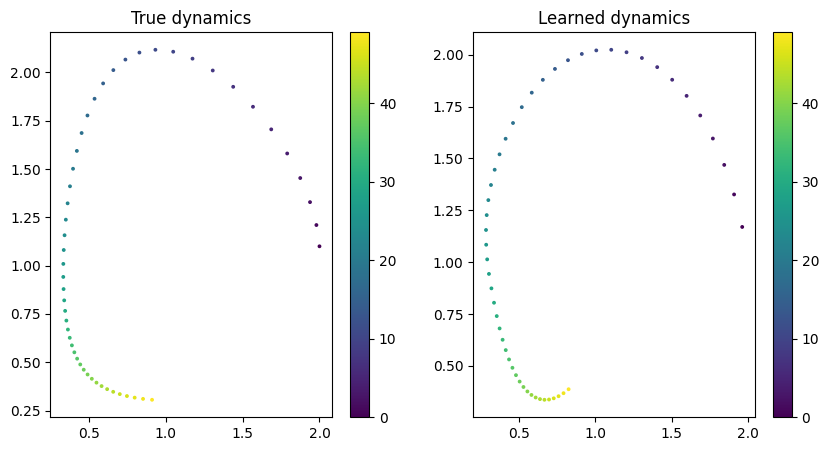
\includegraphics[width=0.75\linewidth]{img/ad.png}
    \caption{Learning the dynamics of an ODE using AD. Left image shows the trajectory of the ODE with the true dynamics, right plot shows the trajectory of an ODE whose dynamics were learned with the adjoint ODE equation.}
    \label{fig:ode-ad}
\end{figure}

Now before we try to optimzie the above code to get better results, there are several things that are very suboptimal in the above code. For one, we have a for loop inside the ode solver, which is something we should always be careful with when using Automatic differentiation. Let us dive a bit deeper into the neural ODE paper and revisit the objective function we want to minimize.

\begin{equation}
\frac{d \mathcal{L}}{d \theta} = \sum_{t \in [0, T]} \frac{\partial \mathcal{L}}{\partial \mathbf{y}(t)} \frac{\partial \mathbf{y}(t)}{\partial \theta}.
\end{equation}

Using the chain rule and some manipulation of the equation, we define the adjoint variable as

\begin{equation}
\mathbf{a}(t) = \frac{\partial \mathcal{L}}{\partial \mathbf{y}(t)}
\end{equation}

and the adjoint ODE as

\begin{equation}
\frac{d\mathbf{a}(t)}{dt} = -\mathbf{a}(t)^T \frac{\partial f(\mathbf{y}(t), t, \theta)}{\partial \mathbf{y}}
\end{equation}

which can be solved using the any ODE solver as before. The gradient can then be computed as

\begin{equation}
\frac{\partial \mathcal{L}}{\partial \theta} = -\int_0^T \mathbf{a}(t) ^T \frac{\partial f(\mathbf{y}(t), t, \theta)}{\partial \theta} dt
\end{equation}

where 

\begin{equation}
\frac{\partial f(\mathbf{y}(t), t, \theta)}{\partial \mathbf{y}} \quad \text{and} \quad \frac{\partial f(\mathbf{y}(t), t, \theta)}{\partial \theta}
\end{equation}

can be computed using AD. The results of the optimization using the adjoint can be seen in figure \ref{fig:ode-adjoint}.


\begin{figure}[h]
    \centering
    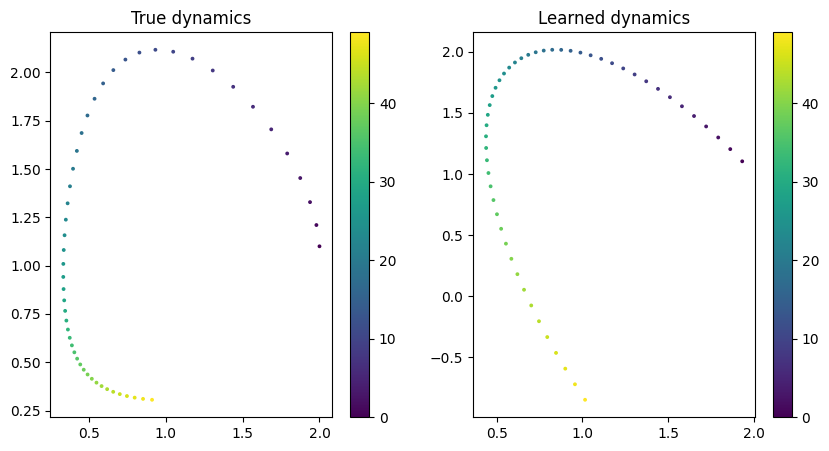
\includegraphics[width=0.75\linewidth]{img/ode_learning.png}
    \caption{Learning the dynamics of an ODE using adjoint ODE. Left image shows the trajectory of the ODE with the true dynamics, right plot shows the trajectory of an ODE whose dynamics were learned with the adjoint ODE equation.}
    \label{fig:ode-adjoint}
\end{figure}

\newpage
\section{Other Neural Network Architectures}
\subsection{Generative Adversial Networks}
\label{CGAN}

Inspired by applications of generative adversial network is cosmology by \cite{bernardini2022ember}, we explored the feasibility of using a conditional generative adversial network (CGAN) \citep{gauthier2014conditional} to generate initial conditions for N-Body simulations. One of the main disadvantages of the CGAN is its unstable training regime. We have implemented an actor and critic in {JAX} \citep{jax2018github} using the neural network library {Equinox} \citep{kidger2021equinox} and trained it on a paintings' dataset. The loss graph that was trained on a painting dataset in figure \ref{fig:gan}. The convergence of the critic and the generator needs to be balanced out in order for the Generator to keep learning over time. 

\begin{figure}[h]
    \centering
    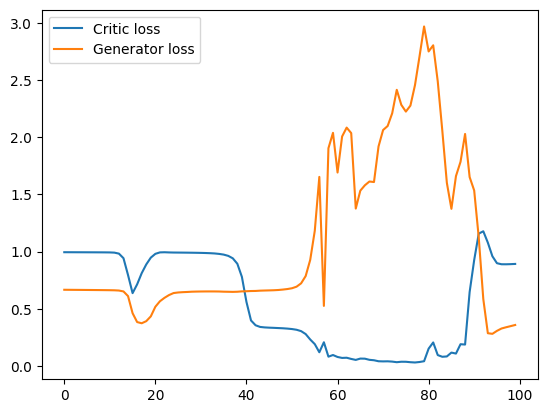
\includegraphics[width=0.5\linewidth]{img/gan.png}
    \caption{Loss values of actors and critics during the training of a GAN on an art dataset.}
    \label{fig:gan}
\end{figure}

\subsection{Encoder Decoder Methods}
\label{encoder-decoder}

Finally, we explored the space of encoder, decoder networks. The main idea is to compress a field into a latent space that is smaller. This can be done by applying a network that first down scales the input data using chained discrete convolutional layers. Then the latent space is reached, which is then upscaled and transformed back into an image using a decoder network consisting of chained transposed convolutional networks. While we were able to train such a network on a paining dataset as sen in figure \ref{fig:ed}, we were not nearly as successful in applying the same strategy for cosmological data. We assume capturing the intricate details of the density field in a latent space is rather challenging, making this approach unsuited for our puposes.

\begin{figure}[h]
    \centering
    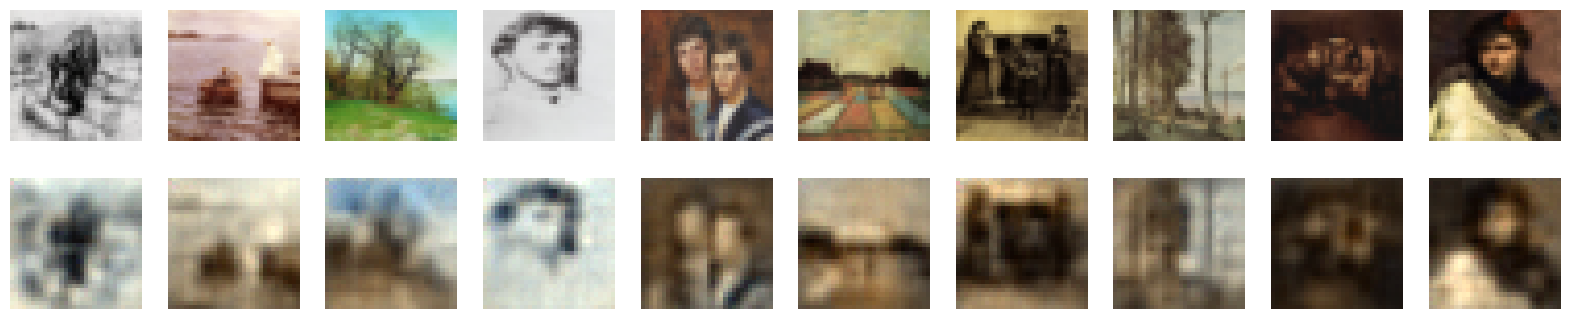
\includegraphics[width=0.75\linewidth]{img/reconstruction.png}
    \caption{Decoding images into latent space and encoding them using trained decoder and encoder networks. Top row shows the original image, bottom row shows an image that was compressed into a latent space with 10\% of the information density.}
    \label{fig:ed}
\end{figure}


\newpage
\section{IC Generation}

\subsection{Optimizing over the Power Spectrum}
\label{optim}

Using the IC generator as implemented in our library JAX, we can generate the IC's for a given power spectrum as seen in figure \ref{fig:cosmax-ic}. The process is described more detailed in section \ref{fig:cosmax-ic}.

\begin{figure}[h]
    \centering
    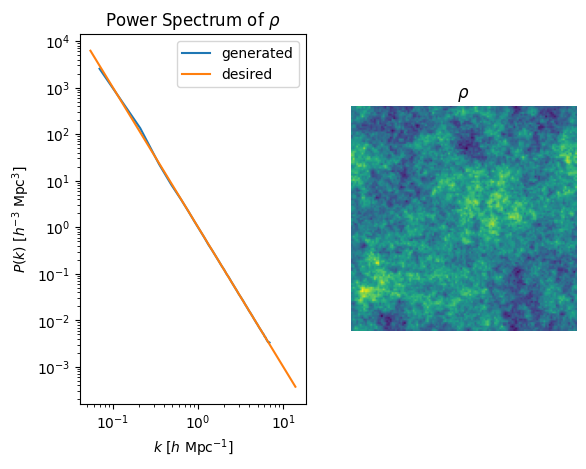
\includegraphics[width=0.5\linewidth]{img/ic_gen.png}
    \caption{Initial conditions as generated with cosmax.}
    \label{fig:cosmax-ic}
\end{figure}

Since the power spectrum is fully differentiable, we can use gradient descent to solve an optimization problem. In this case, we want to find a density field that follows a certain power spectrum, and at the same time has the letters of cosmax stamped into its density field. That means we can generate initial conditions without actually using the IC generator and additionally add more terms to the objective function. We achieve this by using a MSE loss term on the difference between the letters combined with a MSE loss term that quantifies the log deviation of the desired power spectrum, similarly as described in section \ref{ps-loss}.

\begin{figure}[h]
    \centering
    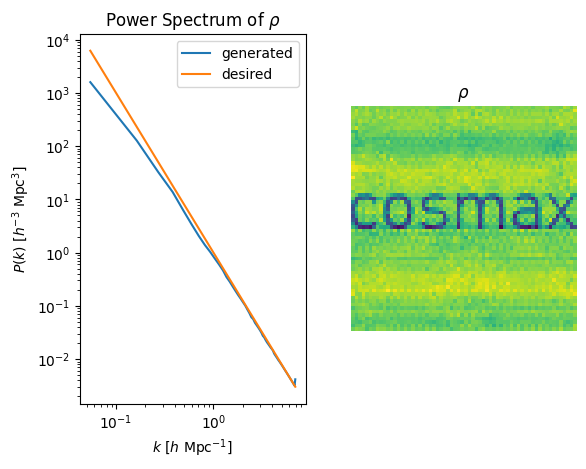
\includegraphics[width=0.5\linewidth]{img/cond_ic.png}
    \caption{Power Spectrum as a loss function to generate conditional IC.}
    \label{fig:cosmax-cosmax}
\end{figure}

\subsection{Conditional White Noise}
\label{white-noise}

Instead of optimizing the density field, we can also optimize the white noise that is then correlated using the IC generator. This is possible, since the IC generator from cosmax is also fully differentiable. In figure \ref{fig:cosmax-white-noise}, we can see a white noise that was optimized specifically to be fed into the optimizer and generate a density field with the desired power spectrum and cosmax letter stamped into its field. The objective function remains the same as in the previous section, however we now optimize the white noise instead of the density fied.

\begin{figure}[h]
    \centering
    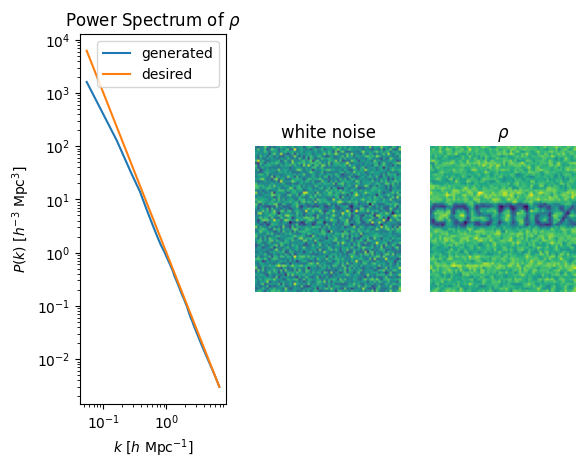
\includegraphics[width=0.5\linewidth]{img/cond_ic_2.png}
    \caption{Power Spectrum as a loss function to generate conditional IC.}
    \label{fig:cosmax-white-noise}
\end{figure}

The interesting part about this, is that the optimized white noise still follows a normal distribution, as seen in figure \ref{fig:white-distr}. However, compared to the process that is described in section \ref{optim}, the convergence of this process is initially faster but cannot reach the same accuracy, even when trained significantly longer.

\begin{figure}[h]
    \centering
    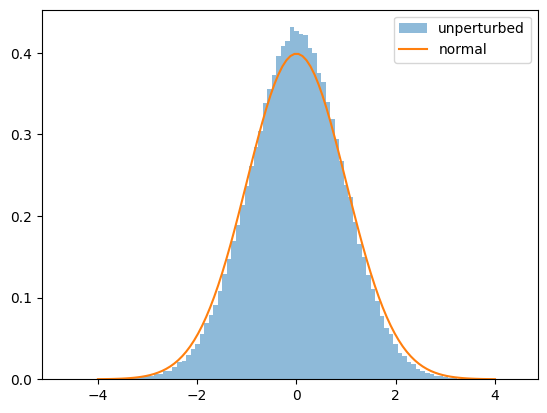
\includegraphics[width=0.5\linewidth]{img/noise.png}
    \caption{Power Spectrum as a loss function to generate conditional IC.}
    \label{fig:white-distr}
\end{figure}


\newpage
\section{Differentiable CIC Mass Assignment}
\label{inverse-map}

To go from a discrete density grid to a set of particle coordinates and masses, we minize the following loss function

\begin{equation}
    L_{IC} = \sum_{\mathbf{y} \in \Omega} \Biggl(\mathcal{A}\Bigl(\mathbf{X}(t_0), \mathbf{m}\Bigr)(\mathbf{y}) - \rho(\mathbf{y})\Biggr)^2.
\end{equation}

Remember the mass vector $\mathbf{m}$ is fixed as the total mass is evenly distributed among the particles. In our case $A$ corresponds to the CIC mass assignment scheme. Hence, we require a differentiable CIC implementation. Using the digitize functions as seen on lines 12-14 we compute nearest grid cell coordinates for all particle positions, which are assumed to be within 0 and 1. Using those, we can compute the CIC assignment weights on lines 15-18. The weights correspond the the overlap of a box over the nearest grid cell. Finally we assign the masses to the weights using index notation. Here we have to compute the assigned mass for 8 additional voxels, as the grid coordinated is rounded down to the integers, meaning the overlapping box can only be crossing over the right boundary of each voxel in each dimension. Leaving us with eight options.

\begin{lstlisting}[language=Python]
@partial(jax.jit, static_argnums=(2))
def cic_ma(
        pos : jax.Array, 
        weight : jax.Array, 
        L : int) -> jax.Array:
        
    dx = 1 / L
    coords = jnp.linspace(start=0, stop=1, num=L+1)

    field = jnp.zeros((L, L, L))

    x = jnp.digitize(pos[0] % 1.0, coords, right=False) - 1
    y = jnp.digitize(pos[1] % 1.0, coords, right=False) - 1
    z = jnp.digitize(pos[2] % 1.0, coords, right=False) - 1

    xw = (pos[0] % 1.0 - coords[x]) / dx
    yw = (pos[1] % 1.0 - coords[y]) / dx
    zw = (pos[2] % 1.0 - coords[z]) / dx

    field = field.at[x, y, z].add(
        weight * (1 - xw) * (1 - yw) * (1 - zw))
        
    field = field.at[(x + 1) % L, y, z].add(
        weight * xw * (1 - yw) * (1 - zw))
    field = field.at[x, (y + 1) % L, z].add(
        weight * (1 - xw) * yw * (1 - zw))
    field = field.at[(x + 1) % L, (y + 1) % L, z].add(
        weight * xw * yw * (1 - zw))
    field = field.at[x, y, (z + 1) % L].add(
        weight * (1 - xw) * (1 - yw) * zw)
    field = field.at[(x + 1) % L, y, (z + 1) % L].add(
        weight * xw * (1 - yw) * zw)
    field = field.at[x, (y + 1) % L, (z + 1) % L].add(
        weight * (1 - xw) * yw * zw)
    field = field.at[(x + 1) % L, (y + 1) % L, (z + 1) % L].add(
        weight * xw * yw * zw)

    return field
\end{lstlisting}

Now that we have a differentiable CIC mass assignment implementation, we need to optimize over it. The entry point is the function fit\_field, it takes the discrete density field domain size $L$, the density field, the total mass the number of optimization iterations and the learning rate. The function then returns a tuple consisting of the Eulerian particle positions $\mathbb{x}$, the Lagrangian particle positions $\mathbf{q}$ and the particle masses $m$. The function return one particle for each grid cell in the field, hence $L^3$ particles.
First we define the Lagrangian particle coordinates using a equilateral grid as defined on line 11. The mass is then evenly distributes among the particles (line 20). After the Adam optimizer is initialized we generate the gradient function of the loss function with respect to the particle position on line 25. We then define the step function, which constitutes a single optimization iteration. There the gradient is computed on line 29, the optimizer computes the parameters updates based on the gradient, and finally the updates are applied to the positions. The step function is then called iterated over and the final values are returned.

\begin{equation}
    \Delta = \frac{\partial L_{IC}}{\partial \mathbf{X}(t_0)}.
\end{equation}


\begin{lstlisting}[language=Python]
def fit_field(
        L : int,
        field : jax.Array,
        total_mass : float,
        iterations : float = 400,
        learning_rate : float = 0.005,
        ) -> Tuple[jax.Array, jax.Array, jax.Array]:

    num_particles = L**3

    pos_lag = jnp.array(jnp.meshgrid(
        jnp.linspace(0, 1, L),
        jnp.linspace(0, 1, L),
        jnp.linspace(0, 1, L)))

    pos_lag = jnp.reshape(pos_lag, (3, num_particles))

    pos = pos_lag

    mass = jnp.ones(num_particles) * total_mass / num_particles

    optimizer = optax.adam(learning_rate)
    opt_state = optimizer.init(pos)

    grad_f = jax.grad(loss)

    @jax.jit
    def step(pos, opt_state):
        grad = grad_f(pos, mass, field)
        updates, opt_state = optimizer.update(grad, opt_state)
        pos = optax.apply_updates(pos, updates)
        return pos, opt_state
    
    for i in range(iterations):
        pos, opt_state = step(pos, opt_state)

    return pos_lag, pos, mass
        
\end{lstlisting}

The loss function simply invokes the CIC mass assignment schemes and computes the MSE between the desired density field and the fitted density field.

\begin{lstlisting}[language=Python]
def loss(
        pos : jax.Array,
        mass : jax.Array,
        field_truth : jax.Array):
    
    fitted_fiel = cic_ma(
        pos,
        mass,
        field_truth.shape[0])
    
    return jnp.mean((fitted_fiel - field_truth) ** 2)
\end{lstlisting}

The optimization process generates the particle positions according to a density field. The result of such a conversion for a density field at $z=0$ can be seen in figure \ref{fig:cosmax-fit}.

\begin{figure}[h]
    \centering
    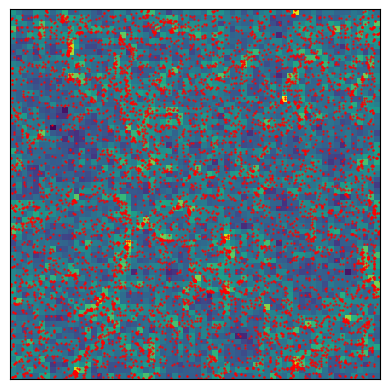
\includegraphics[width=0.5\linewidth]{img/fit.png}
    \caption{Fitting particles to a density field.}
    \label{fig:cosmax-fit}
\end{figure}

In mathematical notation, the above can be expressed as follows. We are given a mass assignment scheme 

\begin{equation}
    \mathcal{A}\Bigl(\mathbf{X}(t_i), \mathbf{m}\Bigr) \colon \mathbb{R}^{3N} \times \mathbb{R}^{N} \rightarrow \mathbb{R}^{L^3},
\end{equation}

where $\mathbf{X}$ is the a tensor stacking all $N$ particle positions

\begin{equation}
    \mathbf{X}(t_i) = \begin{bmatrix}
        \mathbf{X}(0, t_i) \\
        \mathbf{X}(1, t_i) \\
        \dots  \\
        \mathbf{X}(N, t_i)
    \end{bmatrix},
\end{equation}

and $\mathbf{m}$ is the vector of all masses

\begin{equation}
    \mathbf{m}= \begin{bmatrix}
        \mathbf{m}(0) \\
        \mathbf{m}(1) \\
        \dots  \\
        \mathbf{m}(N)
    \end{bmatrix}.
\end{equation}

We can now formulate the the loss function

\begin{equation}
    L_{IC} = \sum_{\mathbf{y} \in \Omega} \Biggl(\mathcal{A}\Bigl(\mathbf{X}(t_0), \mathbf{m}\Bigr)(\mathbf{y}) - \rho(\mathbf{y})\Biggr)^2.
\end{equation}

\begin{figure}[h]
    \centering
    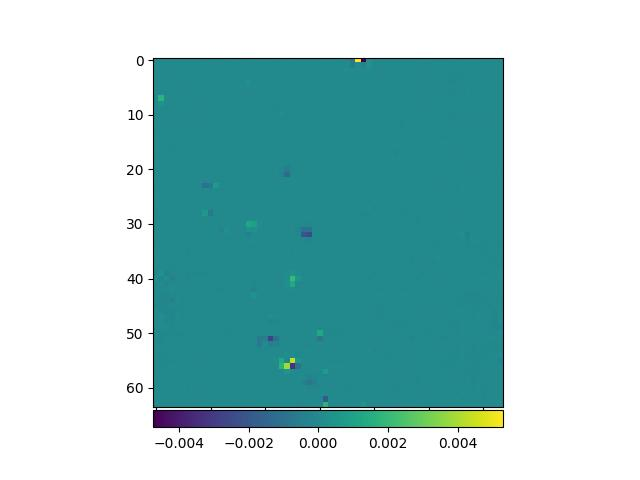
\includegraphics[width=0.5\linewidth]{img/cmp.jpg}
    \caption{Difference between fitted density field an actual density field normalized by dividing through the standard deviation.}
    \label{fig:field-fit}
\end{figure}

In our case the mass vector $\mathbf{m}$ is fixed as the total mass is evenly distributed among the particles. If $\mathcal{A}$ is a differentiable function, we can obtain the gradient using automatic differentiation 

\begin{equation}
    \Delta = \frac{\partial L_{IC}}{\partial \mathbf{X}(t_0)}.
\end{equation}

Now we can leverage the Adam optimizer \citep{kingma2014adam} to optimize the initial conditions.
In our case we have used CIC mass assignment for $\mathcal{A}$. Note that any mass assignment scheme can be used, however it must be a differentiable. This is not the case in the nearest neighbour assignment scheme. The nearest neighbour scheme, assigns all the mass of each particle to the nearest grid cell, hence it is not possible to perturb the particle positions and see a small difference in the distribution, effectively generating non smooth gradients. In this case, the method to choose the initial guess for $\mathbf{X}$ is crucial. As seen before, we can generate intitial conditions using the formula

\begin{equation}
    \mathbf{x} = \mathbf{q} - D_{+}(a)\mathbf{s}(\mathbf{q}),
\end{equation}

whereas $\mathbf{q}$ are the Lagrangian position, which is essential a 3D grid with uniform distances. Therefore if we wish to find $\mathbf{x}$ with the above optimization algorithm, we must choose $\mathbf{X}$ to be a uniform grid. Then we also able to compute the Displacement map $\mathbf{s}$ by reforming the previous equation into

\begin{equation}
    \mathbf{s}(\mathbf{q}) = \frac{\mathbf{q} - \mathbf{x}}{D_{+}(a)}.
\end{equation}

In figure \ref{fig:field-fit} we can observe the accuracy of the method applied to arbitrary sample from the small dataset. The figure shows the difference between the predicted minus the actual density field divided by the standard deviation. Hence a maximum deviation of 0.004 out of 1 is equivalent to a maximum deviation of $0.4\%$.





\end{appendices}
\newpage

\bibliographystyle{plainnat}
\bibliography{reference}

\end{document}
